\documentclass[twoside,a4paper,10pt]{scrbook}

\usepackage{../src/bcthesis}
\usepackage{standalone}
\usepackage[toc]{appendix}

\addbibresource{~/bibliography.bib}
\graphicspath{{../figures/}}
\usepackage[final]{pdfpages}
\usepackage{../src/illcmolthesis}
\usepackage{xcolor}
\usepackage{etoc}
\usepackage{multicol}
\deftocheading{toc}{}%

\renewcommand{\parttitle}[4]{{%
	% Page style
	\color{main}\sffamily%
	%
	% Title 
	\chapter[#1]{\textsc{\color{black}\thechapter} #2}\label{ch:#3}

	% Abstract
	\fontsize{12pt}{2em}\selectfont{\noindent#4}\par
	\vfill

	{\color{black}\normalsize%
%		\noindent\textbf{Contents}
		\localtableofcontents
	}
	
	% Style this page and start new one
	\thispagestyle{empty}
	%\pagecolor{main}
	\newpage%\pagecolor{white}
}}

\setkomafont{chapter}{%
	\color{main}%
	\fontsize{60pt}{1em}\selectfont\bfseries
}
\renewcommand*{\chapterheadstartvskip}{}
\renewcommand*{\chapterformat}{}%
\renewcommand*{\showbibliography}{}

\begin{document}

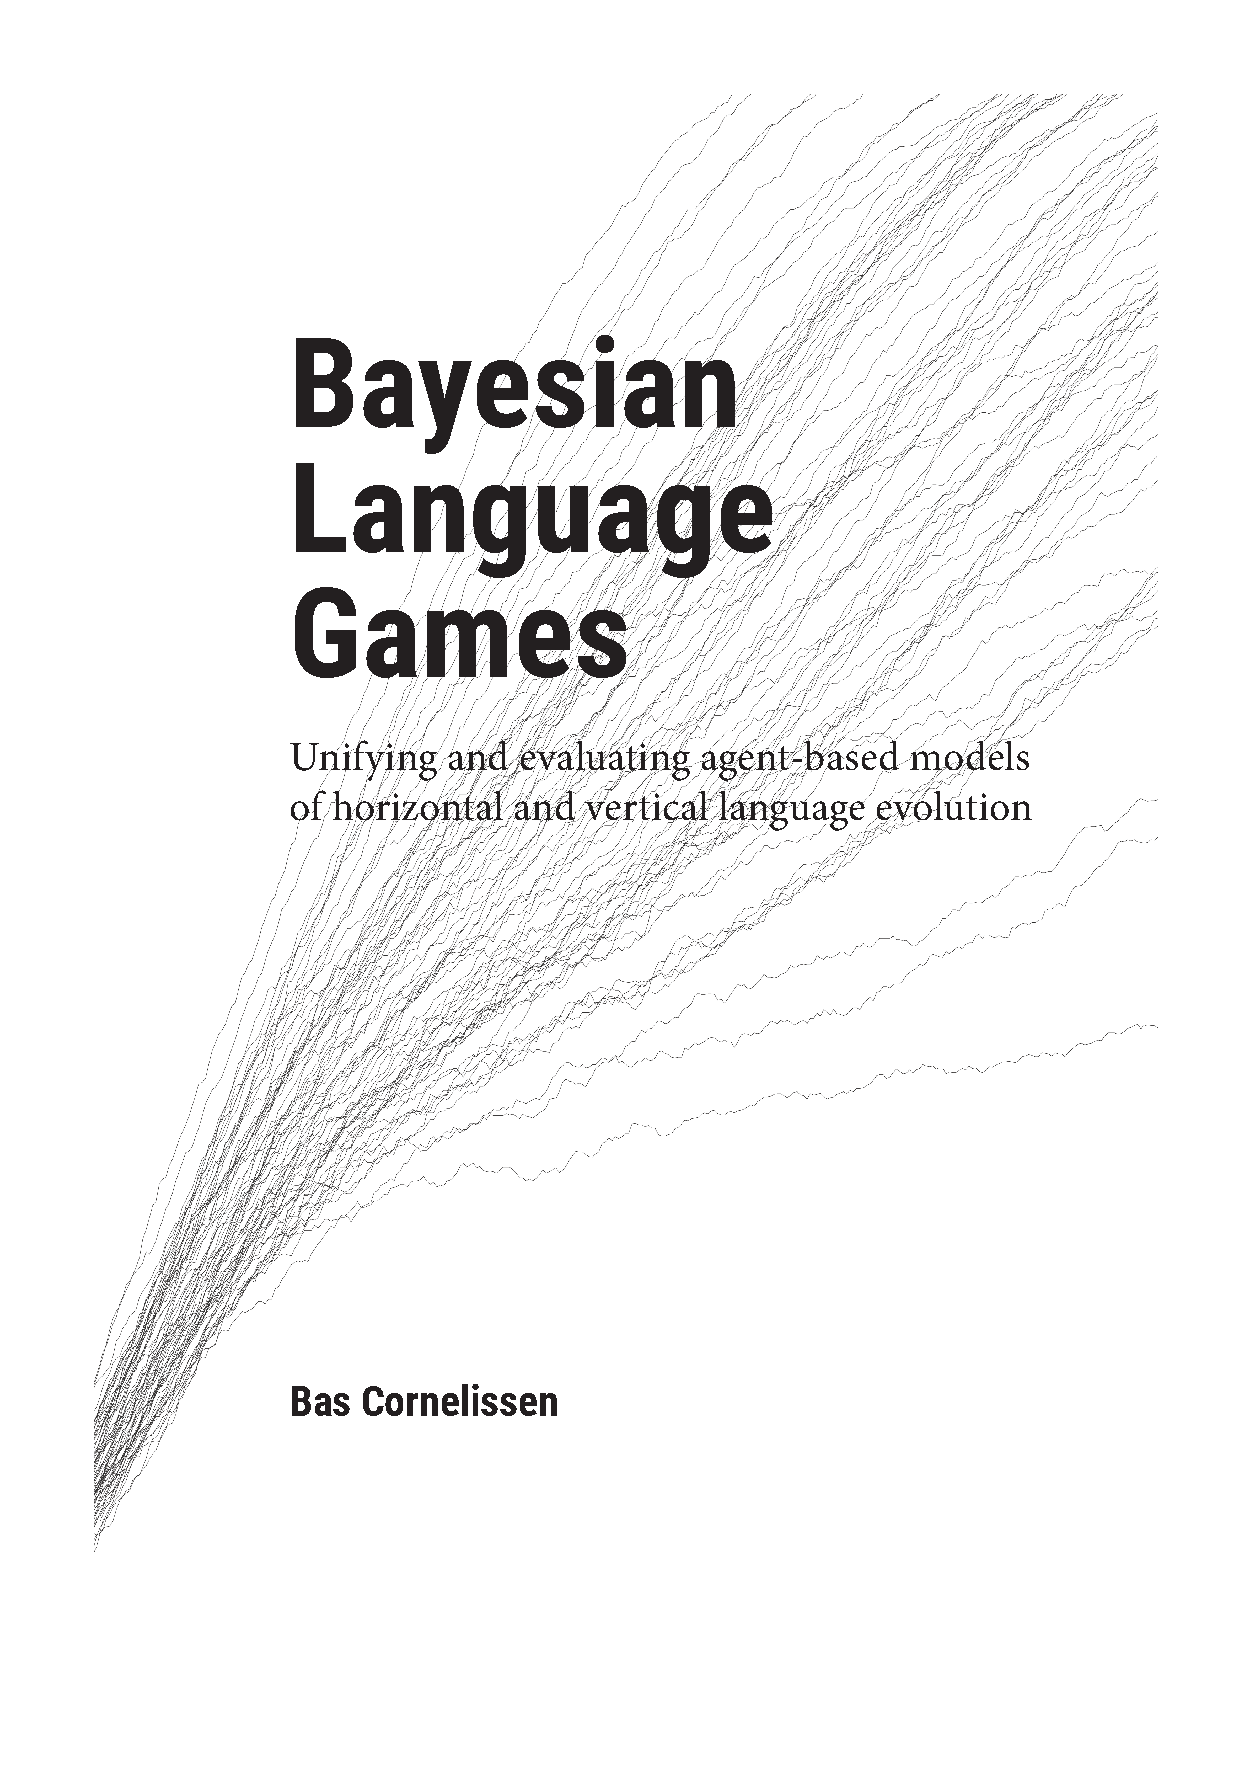
\includepdf{../00-cover/Cover}


\title{\textbf{Bayesian Language Games}\\Unifying and evaluating agent-based models\\ of horizontal and vertical language evolution}
\author{Bas Cornelissen}
\birthdate{26 February 1992}
\birthplace{Utrecht}
\defensedate{30 August 2017}
\supervisor{Willem Zuidema}
\committeemember{prof.~dr.~Frank Veltman}
\committeemember{dr.~Wilker Aziz}
\committeemember{prof.~dr.~Benedikt Löwe}
\maketitle	


\mbox{}
\thispagestyle{empty}
\newpage


{\sffamily{{\fontsize{12pt}{2em}\selectfont{\noindent\color{main}%
\textbf{Abstract.\;\;} Human language is one of the most intricately structured communication system in the natural world.
	Over the last decades researchers in various fields have developed the idea that languages are primarily shaped by processes of cultural evolution, and that these processes can account for the structure of language.
	Computational models play an important role in their arguments.
	This thesis asks what those models can teach us about cultural language evolution.
	To that end, the first part of this thesis connects the two main branches of agent-based models, naming games and iterated learning, in a new \emph{Bayesian language game}.
	The game gives a unified view on the field and suggests a characterisation of the behaviour exhibited by the main agent-based models of language evolution.
	It moreover addresses shortcomings of earlier models. 
	We find lineage-specific languages reflecting the innate biases of the learners.
	The second part of this thesis aims to compare that behaviour with the evolution of actual language.
	Numeral systems are argued to be an ideal empirical test case for models of cultural language evolution.
	We revisit Hurford’s pioneering work on the modelling of the emergence of numeral systems, and discuss some further results.
	
	
	\vfill
	\noindent
	\textbf{Preface.\;\;}
	Dear reader, 
	I will keep it short. 
	As I write, my mother is preparing a delicious meal. And, as you will understand, I cannot keep my parents waiting. 
	They haven't seen me much over the last few months, and I'm afraid they are not the only ones.
	Let me just say thanks to all those wonderful, warm, and loving people that make life so much fun.
	Oh and Jelle, of course, thanks for putting up with me ;-)
\thispagestyle{empty}	

}}}}



\mbox{}
\thispagestyle{empty}
\newpage


\tableofcontents

% Chapter 1: Introduction
\documentclass{../src/bcthesispart}
\title{The cultural origins of language}
\author{Bas Cornelissen}
\begin{document}

%——————————————————————————————————————————————————————————
\parttitle{The cultural origins of language}%
	{The cultural origins of language}%
	{The cultural origins of language}{}
%——————————————————————————————————————————————————————————




\noindent
Communication abounds in the natural world, but few, if any, communication systems are so intricately structured as human language.
We can understand the meaning of a sentence that has never been uttered before, because we understand the words it consists of and the way in which they are combined — that is to say that language is by and large \emph{compositional}.
The words, morphemes, themselves also have an internal structure: they consist of phonemes, combined in a accordance with a combinatorial, phonological system specific to the language.\nocite{Zuidema2013}
The semantic and phonological combinatorics together give language what \textcite{Hockett1960} dubbed a ‘duality of patterning’ — a design feature not commonly found in communication systems of other species.
Most animal communication systems are \emph{holistic}: every vocalisation has one specific function, and no further internal structure \parencite{Zuidema2013}.
There are, it seems, few interdependencies between vocalisations.
But language is quite different: just about any two sentences will have many interdependencies in their phonology, morphology, hierarchical structure, and so on. 
It is in this sense that language has a distinct \emph{systematicity} \parencite{Kirby2017}.
%%




Now, the Big Question is this: where does it come from? 
And, indeed, why only us?
Well, we find ourselves in good company.
Robert Berwick and Noam Chomsky (2017) \nocite{Berwick2017} have been thinking about the same question, and leave us no doubt how we should \emph{not} try to account for the structure of language: “by means of a cultural-biological interaction”.
No, “this latter effort fails in all respects”.
Some of that work is “trivially inadequate”, or otherwise the “Kirby-type models”, “the Kirby work” and “the Kirby line of research” do of course “not say anything about the initial origin of compositionality”.
%%




Good, good! More than enough reason to write a thesis about this “Kirby type work” — and in passing perhaps even cite more than two of his papers. 
But let’s leave the polemics there. After all, what greater good do they really serve?
%%



\textcite{Berwick2017} raise some fair concerns, for example regarding the testability and empirical validity of the Kirby-type theories.
Or regarding their explanatory power: if your ‘agents’ already know, say, context-free grammars, and they ‘evolve’ a compositional language, does your model explain anything?
Are you then, if anything, addressing the evolution of universal grammar, or just modelling language change? 
These are all valid concerns — or so I think, since I address some of them in this thesis, too.
But reading Berwick and Chomsky’s paper — I haven’t read the book yet — one starts to understand what it means if two scientific traditions have lost their common ground and have started talking about radically different things, only superficially using the same words.
%%




%——————————————————————————————————————————————————————————
\bigbreak\noindent
My apologies if I overwhelmed the reader with this, well, lack of introduction, but I want to get started sooner rather than later.
One should know that the Kirby-type theories, in the broad sense, are really the work of a large group of linguists, cognitive scientists, biologists, anthropologists, computer scientists, statisticians, and even physicists, who over the last 30 years or so have tried to turn the question of language evolution upside down.
The ‘traditional’ debates centred around the question whether language was an adaptation or not. 
Does language perhaps add to our reproductive fitness, or was it a key mutation event that catapulted language in the world?
In either case, the origin of language was thought to be a fundamentally biological concern.
We only had to find out how those brains evolved to accommodate language.
Well, the Kirby-type work turned that around: how do languages have to change, in order to fit in our brains \parencite{Christiansen2016a}?
Rather than evolving brains, let’s think about evolving languages.
%%





For this to even make sense, one has to drastically change the, let's say, Chomskyan conception of language.
Language now becomes a complex adaptive system in its own right, that is subject to all kinds of pressures, at multiple different levels and timescales simultaneously \parencite{Kirby2002,Christiansen2016a,Smith2014,Kirby2017,Steels2016}.
On a biological level and evolutionary timescale the innate mechanisms that underly human cognition and language need to develop. 
At an individual level and much shorter timescale, humans acquire language, constrained by what their biological makeup can accommodate.
These learning biases influence, on a cultural level and historic timescale, the cultural dynamics of language.
Universals that emerge through processes of cultural evolution in turn shape the fitness landscape and indeed, interactions exist within in and across all levels.
Rather than looking solely at the biology of language, the question is how it can interacts with acquisition and use.
The idea developed is that “language has been adapted through cultural transmission over generations of language users to fit the cognitive biases in inherent in the mechanisms used for processing and acquisition” \parencite[12]{Christiansen2016}. \nocite{Tomasello1999}
%todo (optional) include figure from Kirby?
%%




Returning to \textcite{Berwick2017}, I think they are quite right to point out that this work “does not really tackle questions about the evolution UG, but rather questions about how particular languages change over time, once the faculty of language itself is in place”.
I doubt Kirby would disagree.
Indeed, this is the entire point.
Since if it turns out that particular languages tend to change over time in a somewhat systematic way that \emph{explains} their structure, then the explanatory burden is lifted from the faculty of language.
And this is precisely what the Kirby-type theories argue for: that biology does not have to carry the entire explanatory load, but that a fair share of linguistic structure can be explained by a process of \emph{cultural evolution}.
As \textcite{Kirby2017} concludes, “we expect the language faculty to contain strong constraints only if they are domain general (e.g.\ arising from general principles of simplicity) and that any domain-specific constraints will be weak.”
If anything, the Kirby-type work is in the business of explaining away UG, rather than explaining it.
%%




%——————————————————————————————————————————————————————————
\bigbreak\noindent
Now, the evolution of language is a notoriously hard problem — I belief this is where one is supposed to mention the \emph{Société} — but how does one go about if language is moreover a complex adaptive system?
Using mathematical and computational models is one solution.
Modelling makes all assumptions absolutely transparent, allows one to verify their coherence and consistency and generate new hypotheses, or even predictions \parencite{Jaeger2009}.
Accordingly, models have figured prominently in the literature on cultural language evolution.
And that is where the habitat of this thesis is to be found.
\emph{What can these models of language evolution actually learn us about language evolution?}
That is the heart of this thesis, but as such, the question is too open ended. 
I therefore break up the question in two parts.
%...
\begin{enumerate}
	\item \emph{What kind of \emph{behaviour} can we expect from \emph{agent-based} models of language evolution?}
	%——————————————————————————————————————————————————————————
	To answer this question, I aim to formulate a model that captures a substantial share of the agent-based modelling tradition, and try to characterise its behaviour.
	The ‘substantial share’ is easily identified, since the field falls apart in two (strictly separated) traditions. 
	\textbf{Chapter \ref{ch:iterated-learning}} introduces the ‘vertical’ tradition around \emph{iterated learning}.
	This is the Kirby-type work that addresses how vertical transmission between generations can shape language. 
	\textbf{Chapter \ref{ch:naming-games}} introduces the ‘horizontal’ tradition around \emph{naming games}, which focusses on the self-organising power resulting from local interactions within a generation.
	Although the traditions are strictly separated, I will argue in \textbf{chapter \ref{ch:bayesian-naming-games}} that their models are very similar.
	To do so, I take inspiration from Bayesian models of iterated learning and propose the \emph{Bayesian language game}. 
	By further changing the population model I can interpolate between both traditions and thus analyse their behaviour in a single unified framework.
	I moreover argue that it addresses some of the problems left open by Bayesian models of iterated learning.
	
	\item \emph{How does that behaviour relate to actual evolved language?}
	%——————————————————————————————————————————————————————————
	Once it is clear what kind of behaviour these agent-based models exhibit, one should ask what this learns us about language evolution.
	But how can one start answering such a question without an empirical test case?
	In \textbf{chapter \ref{ch:numerals}} I therefore argue that numeral systems are a good test case, and explain in some detail what the structures are one should try to explain.
	In \textbf{chapter \ref{ch:counting-games}} I make a first start with simulating the emergence of numeral systems, which largely amounts to revisiting and extending the pioneering work of James Hurford.
\end{enumerate}
%...
The reader might want to note that the summaries at the start of every chapter further flesh out this outline.



The problem of language evolution challenges many disciplinary boundaries.
This thesis alone borders at least several branches of linguistics, statistical physics, biology, probability theory and Bayesian (cognitive) modelling.
When starting with the current work, I was new to pretty much all of these fields (except perhaps some courses in the latter two fields) and many important results might very well have escaped my attention. 
But some things I deliberately left out, or only touch on in passing.
These include (1) models of biological evolution, (2) evolutionary game theory, (3) genetic algorithms, (4) evolution of \textsc{ug}, (5) empirical studies of transmission chains and (6) experimental semiotics.
Neither will I further discuss broader debates, of which the Berwick and Chomsky paper is part.
Instead, I try to address issues in the field of agent-based modelling of language evolution on its own terms.
Indeed, the reader will notice that focus in the majority of this thesis is decidedly on the models, more so than on possible interpretations thereof.
This partly reflects personal interest, but more importantly, I belief interpretations of models should, insofar as possible, built on a sound understanding of the model themselves.
That is what I hope this thesis, if anything, contributes to.





%——————————————————————————————————————————————————————————
\paragraph{Source code and data}

I have made the source code of all experiments publicly available via \href{http://bascornelissen.nl/msc-thesis/}{bascornelissen.nl/msc-thesis} (including all figures and LaTeX files).
A reference to the ‘raw’ data from all experiments can also be found there.
The captions of many figures contain a code like \figid{BNG06} or \figid{FIG03}.
This identifies the experiment or figure in the repository.




%——————————————————————————————————————————————————————————
\paragraph{notation}

Throughout the thesis I use several notational conventions.
Vectors are written in boldface, as in $\vect x = (x_1, \dots, x_K)$, and indexed by $k$ if they have length $K$.
Sometimes it will be convenient to abbreviate $x_0 := \sum_{k=1}^K x_k$.
We often need to decorate variables with time-indications. The most consistent unambiguous solution, $\vect x^{(t)}, x_k^{(t)}$ etc., often clutters the notation.
Therefore, vectors (boldface) simply get their indication in the subscript ($\vect x_1, \vect x_2, \dots, \vect x_t, \dots$) and I only use the superscript $(t)$ when confusion can arise, as in $x_k^{(t)}$. 
If $X$ is a random variable with distribution $\text{Dist}$ parametrized by $\lambda$, then by $X \sim \text{Dist}(\lambda)$ we mean that $p_X(x) = \text{Dist}(x \mid \lambda)$ where the latter is the density (mass) function.
%For discrete random variables we also write $p(X = x) = p_X(x)$.
We mostly drop the random variables and write $p(x)$ and $p(x \mid z)$ rather than $p_X(x)$ and $p_{X\mid Z}(x \mid z)$.
Normalizing constants are often irrelevant and we write $p(x) \propto f(x)$ to indicate proportionality, i.e.\ that $p(x) = \nicefrac{1}{C} \cdot f(x)$ where $C$ does not depend on $x$.
With regard to sets, $\mathbb{N}, \mathbb{Z}, \mathbb{R}$ denote the natural numbers, integers and reals. 
If $A$ and $B$ are sets, their Cartesian product is $A\times B$ and $B^A$ denotes the set of all functions $f: A \to B$.
‘Spaces’ typically have a calligraphic character, so $x$ lies in $\XX$ and parameters tend to be Greek.
Finally, $x$ is nearly always an observable variable (e.g.\ an utterance), $z$  and unobservable variables (e.g.\ internal representation of a language), $m$ a meaning and $s$ a signal.

%——————————————————————————————————————————————————————————
\showbibliography

\end{document}


%\part{Agent-based models of cultural language evolution}

%Chapter 2: Iterated learning
\documentclass{../src/bcthesispart}
\title{Iterated Learning}
\author{Bas Cornelissen}
\begin{document}
%——————————————————————————————————————————————————————————

\parttitle{Iterated Learning}%
	{Iterated Learning}%
	{iterated-learning}{%
	% Abstract
	%---------
	Could it be that structure in language emerges because it is transmitted from one generation to the next?
	Is cultural \emph{transmission} the force shaping language?
	Early models of iterated learning suggested precisely that.
	Bayesian models improved the early work by separating the biases of the learners from the effects of transmission.
	But they also indicated that cultural evolution only allows the prior biases to surface, a result that sparked a small controversy.
	The ‘convergence to the prior’ was shown to break down in more complicated populations, again creating room for the shaping force of cultural evolution.
	This chapter introduces the iterated learning tradition and ends with a list of desiderata for models of cultural language evolution.
	The list serves as a guide to the remainder of this thesis.
}
%——————————————————————————————————————————————————————————




%——————————————————————————————————————————————————————————
%——————————————————————————————————————————————————————————
\section{Early iterated learning models}
%——————————————————————————————————————————————————————————
%——————————————————————————————————————————————————————————


In the early years of this century, James Hurford, Simon Kirby, Kenny Smith and others, developed the idea that cultural transmission, in the form of \emph{iterated learning} (\textsc{il}), could be the source of structure in language.
Early work in this tradition tried to isolate a “minimal set of assumptions and hypotheses with which linguistic structure can be explained”  \parencite{Brighton2002}.
The result was a simple model of cultural transmission between generations consisting of a single agent each.
In the model, language alternates between an internal representation (\textsc{i}-language in Chomskyan parlance; \cite[19--24]{Chomsky1986}) or an external representation in the form of actual utterances (\textsc{e}-language), as figure \ref{fig:iterated-learning-illustration} illustrates.
The first agent (the parent) is presented with several objects for which it produces some utterances.
Those utterances form the primary linguistic data from which the second agent (the child) has to learn a language.%
	\footnote{%>>>
	The utterances alone are not enough, unless you assume the child can mind-read. Instead meaning-signal pairs are often communicated.
		\label{fn:mind-read}
	%<<<
	}
The child goes on to become the parent of the next generation, forms expressions for several (other) objects, which are observed by the next agent, and so on.
%%




%- - - - - - - -
\begin{SCfigure}
	%\documentclass{../src/bcthesispart}
%\begin{document}
\begin{tikzpicture}[scale=.8]\sffamily\footnotesize
	\tikzset{lang/.style={draw, circle, fill=main!20}}
	\tikzset{obs/.style={draw, circle, fill=main}}
	\tikzset{produce/.style={thick,draw,->}}
	\tikzset{induce/.style={thick,draw,->,dashed}}
	\tikzset{brace/.style={decoration={brace,mirror,raise=10pt}, decorate}}
	
	\path 	(1,2)  node[lang] (z1) {$\lang_1$}
			(3,0)  node[obs]  (x1) {$\obs_1$}
			(5,2)  node[lang] (z2) {$\lang_2$}
			(7,0)  node[obs]  (x2) {$\obs_2$}
			(9,2)  node[lang] (z3) {$\lang_3$}
			(11,0) node[obs]  (x3) {$\obs_3$};			
	\draw[induce]  (0,1) -- (z1);
	\draw[produce] (z1) -- node[midway, above, sloped] {\textsc{produce}} (x1);
	\draw[induce]  (x1) -- node[midway, below, sloped] {\textsc{learn}} (z2);
	\draw[produce] (z2) -- (x2);
	\draw[induce]  (x2) -- (z3);
	\draw[produce] (z3) -- (x3);
	\draw[induce]  (x3) -- (12,1);
	
	
	\node[align=left, text width=1.5cm] at (-2,2) 
		{Language (internal)};
	\node[align=left, text width=1.5cm] at (-2,0) 
		{Utterances (external)};			
		
	\def\bracey{-.5}
	\def\delta{.05}
    \draw [brace] (0+\delta,\bracey) -- (4-\delta,\bracey) 
    	node [pos=0.5, yshift=-.7cm] {Generation 1}; 
    \draw [brace] (4+\delta,\bracey) -- (8-\delta,\bracey) 
    	node [pos=0.5, yshift=-.7cm] {Generation 2}; 
    \draw [brace] (8+\delta,\bracey) -- (12-\delta,\bracey) 
    	node [pos=0.5, yshift=-.7cm] {Generation 3};
\end{tikzpicture}	
%\end{document}

	
	\caption{%
	In the iterated learning model, the language produced by the previous generation serves as the primary linguistic data for the next.
	%----------
	\figdetails{Adapted from \textcite{Kirby2001}.}
	\label{fig:iterated-learning-illustration}}
\end{SCfigure}
%- - - - - - - -




Every generation learns a language by observing the language of the previous generation, who themselves learned it from the generation before them.
The target of learning is therefore the outcome of the same learning process and this gives rise an evolutionary dynamics on the cultural level:
the fact that a language has to be learned over again shapes the language itself to become better learnable, hence better transmissible.
And key to better transmission, many studies suggested, was the acquisition of some form of systematicity.
Paraphrasing \textcite{Hurford2000}, language appeared to be structured, because cultural transmission favours systematicity.
%%



%——————————————————————————————————————————————————————————
\paragraph{the emergence of compositionality, i}

This conclusion was primarily based on computer simulations of the emergence of compositionality which I briefly want to discuss.
Suppose, following \textcite{Brighton2002}, that agents are positioned in an environment with various objects.
The objects have $F$ possible features, each taking $V$ values, and thus correspond to points in a $F$-dimensional meaning space $\mathcal{M}$.
The features might be color and shape, taking values triangular, rectangular or circular and orange, blue and black respectively.
A language associates meanings $m \in \mathcal{M}$ to signals $s$ in a space $\mathcal{S}$ of signals, typically strings over some alphabet.
Certain languages are compositional, meaning that the signals can be decomposed in subsignals that each bear one aspect of the meaning.
Compositional languages should be distinguished from \emph{holistic} languages where meanings correspond to a signals without there being any underlying regularity.




Consider the following language with alphabet $\{t,r,c, \;o,b,k\}$: 
%-
\begin{align*}
	(\triangle, \orcl) \mapsto to, 	
		\quad (\triangle, \bluecl) \mapsto tb
		\quad (\triangle, \blcl) \mapsto tk \\
	(\square, \orcl) \mapsto so, 	
		\quad (\square, \bluecl) \mapsto sb
		\quad (\square, \blcl) \mapsto sk \\
	(\Circle, \orcl) \mapsto co, 	
		\quad (\Circle, \bluecl) \mapsto cb
		\quad (\Circle, \blcl) \mapsto ck 
\end{align*}
%-
This language is clearly compositional, since the first subsignal indicates the shape, ($t$riangle, $r$ectangle, $c$ircle) and the second subsignal the color ($o$range, $b$lue, blac$k$).
In fact, that description is much more efficient:
%-
\begin{align*}
	&\triangle  \mapsto t, 	
		\quad \square \mapsto s,
		\quad \Circle \mapsto c \\
	&\orcl \mapsto o, 	
		\quad \bluecl \mapsto b
		\quad \blcl \mapsto k
\end{align*}
%-
Rather than listing the signals corresponding to each of the $V^F = 3^3$ meanings (the worst case scenario for a holistic language), a compositional languages can be \emph{compressed} to $F\cdot V = 2\cdot 3$ rules listing to which \emph{sub}signal every feature maps.
That also means that one can faithfully reconstruct a compositional language from $F\cdot V$ signals, whereas it would need to observe \emph{all} signals to reconstruct a holistic language (in the worst case).
A compositional language is, in short, more \emph{compressible} and as a result better \emph{transmissible}.
%This observation will be crucial for understanding the \ilm{}.




%——————————————————————————————————————————————————————————
\paragraph{Transmission bottlenecks and generalisation}

In reality, children do not observe their entire language (e.g.\ all English sentences), but only a subset of it.
They face a \emph{transmission bottleneck}%
	\footnote{%>>>
	In fact, various different bottlenecks have been put forward; see \textcite[ch. 4]{Cornish2011} for an overview and a discussion of the empirical findings regarding the presence of such a bottleneck.		
	%<<<
	}
better known as the \emph{poverty of the stimulus}.
If there is no such bottleneck all languages can be transmitted in their entirety, and faithfully so.
The language can consequently not be changed by transmission and the initial language marks a \emph{steady state}, maintained throughout all future generations.
In the presence of a bottleneck, however, the learner is forced to \emph{generalize} the observed data to a full language, in which case systematic errors can slowly accumulate.
%%




The exact generalisation mechanism can take many different forms, such as (heuristic) grammar induction \parencite{Kirby2001,Zuidema2003}, training a neural network \parencite{Kirby2002,Smith2002a} or constructing a finite state transducer \parencite{Brighton2002}.
All these mechanisms try to discern some structure (e.g.\ compositionality) in the language.
Sometimes, that allows the child to produce signals for unobserved meanings.
But in other cases, the child is forced to invent a new signal. 
Incidentally, the new signal introduces a structure previously absent in the language.
The next generation is then more likely to infer a language that reproduces that structure.
As time passes, the differences between successive generations shrink and the language becomes more and more stable:
the transmission bottleneck forced the language to become better transmissible.
This is how the poverty of the stimulus solves the poverty of the stimulus \parencite[cf.][]{Zuidema2003}.
%%




A variety of different models confirmed this account.
To name a symbolic and connectionist example, \textcite{Kirby2001} showed that a bottleneck caused the emergence of a stable, compositional language in agents representing language with definite-clause grammars.
In another study, \textcite{Kirby2002} found that the number of training instances passed between neural-network agents acted as a bottleneck, with a medium-sized training set leading to structured meaning-signal mappings.
The fact that these, and many other, different models gave rise to similar behaviour is in itself striking.
But it also makes it difficult to decipher what exactly is going on.





The shape-color example gives a hint, since there is a language much more compressible than a compositional one: the degenerate language that expresses \emph{every} meaning with the same signal. 
The fact that none of the early studies seem to have produced degenerate languages, suggests that a bias against those must have been present \parencite{Cornish2011}.
%--> “Cornish (2011) argues that in fact all simulatiosns of iterated learning purporting to demonstrate the emergence of compositionality have in some way implemented a constraint that rules out degeneracy”
\nocite{Culbertson2016}
Or, conversely, that the learning algorithms implicitly pressured towards compositional languages.
This opens up the possibility that “cultural evolution does no more than transparently map properties of the biology of an individual to properties of language” \parencite{Kirby2017}.
Kirby points out that there are reasons to doubt this conclusion:
The size of the bottleneck and the structure of the domain for example influence the simulations.
Nonetheless, it became clear that in order to make claims about the shaping force of cultural evolution, one needs to know 1) what the \emph{implicit biases} in the model are, 2) what the biases of the agents are and 3) how those interact with the cultural process.
%%




%——————————————————————————————————————————————————————————
%——————————————————————————————————————————————————————————
\section{Iterated learning with Bayesian agents}
%——————————————————————————————————————————————————————————
%——————————————————————————————————————————————————————————


In 2005, Thomas Griffiths and Michael Kalish reinterpreted the iterated learning model in a population of Bayesian agents\nocite{Griffiths2005,Griffiths2007}.
One reason for doing so is that it connects the iterated learning model to a rich Bayesian modelling tradition in cognitive science \parencite[see e.g.][]{Perfors2011,Goodman2016,Griffiths2008} and the formal models of human behaviour that have been proposed there.
The Bayesian model of Griffiths and Kalish also solved the issues arising from implicit biases, since it \emph{explicitly} encodes the biases of the learners.
Moreover, the authors managed to characterise the long-term behaviour of the model — \emph{convergence to the prior} — which sparked a small controversy.
In the years that followed, the Bayesian paradigm appears to have surfaced as the primary approach to modelling iterated learning \parencite{Kirby2014,Kirby2017}.
For that reason, and for its role in the next chapter, I want to go through the model in detail.




Recall from figure \ref{fig:iterated-learning-illustration} that in iterated learning, a language alternates between a ‘latent’ internal representation $\lang$ and an ‘overt’ external representation $\obs$.
Agents use a \emph{production} and \emph{language algorithm} (\PA{} and \LA{}) to move between these representations.\footnote{%
	%>>>
	The language algorithm is usually called a \emph{learning} algorithm.
	Since that terminology causes some confusion in chapter \ref{ch:bayesian-naming-games}, I use the term \emph{language algorithm}.
	%<<<
	}
The idea put forward by \textcite{Griffiths2007a} is to model these production and language algorithms with probability distributions.
An agent using language $\lang_t$ has a distribution $p_{\PA}(\obs_t \mid \lang_t)$ over productions describing how to select a utterance. 
Conversely, it has a distribution $p_{\LA}(\lang_t \mid \obs_{t-1})$ from which the agent picks a language after observing data $\obs_{t-1}$ produced by the previous agent.
Note that, as figure \ref{fig:iterated-learning-illustration} illustrates, these are the only dependencies. 
Productions are conditionally independent from previous productions and the same goes for languages.
This seems reasonable as an agent cannot use the previous production when making a new one (only its representation thereof) and clearly an agent cannot use the \emph{unobservable} language of the previous agent directly.
In short, iterated learning becomes a stochastic process on the random variables $\obs_t$ and $\lang_t$, which are conditionally independent from previous $\obs_t$’s and $\lang_t$’s respectively.




What makes these agents ‘Bayesian’ is that their language algorithm reuses the the production algorithm and the prior beliefs of the agents using Bayes’ rule.
When confronted with data $\obs_t$, the agents infer the \emph{posterior} distribution
%-
\begin{align}
	p(\lang_t \mid \obs_{t-1}) 
		\propto p_{\PA}(\obs_{t-1} \mid \lang_t) 
			\cdot p(\lang_t),
\end{align}
%-
which captures how likely every language $\lang_t$ is in light of the observed the data. 
The posterior distribution balances two factors. 
First --- and this is where the production algorithm is reused --- how probable the agent itself regards the observed data to be, if it were to use language $\lang_t$. This is the \emph{likelihood} term $p(\obs_t \mid \lang_t)$. 
And second, how likely the language is in the first place: the \emph{prior} $p(\lang_t)$.
%%




Interestingly, \emph{before} Griffiths and Kalish published their Bayesian interpretation, \textcite{Kirby2004} also noted that the language acquisition can be seen as Bayesian inference.
The prior, they state, corresponds to Universal Grammar or the Language Acquisition Device: “everything the learner brings to the task \emph{independent of the data}” (italics in original). 
However, \textcite{Griffiths2007a} stress that the prior “should not be interpreted as reflecting innate constraints \emph{specific} to language acquisition” (my italics).
The prior is, in other words, not necessarily domain specific, but aggregates all factors that influence language acquisition, including learned biases.
Therefore, “the prior is better seen as determining the amount of evidence that a learner would need to see in order to adopt a particular language”. 
Nevertheless many later papers use the prior primarily to capture innate learning biases \parencite[e.g.][]{Kirby2014,Kirby2017}.
%%




So how does a Bayesian agent adopt a particular language?
\textcite{Kirby2004} assume agents pick the language with the highest probability under the posterior, the \emph{maximum a posteriori} (\MAP) estimate $\argmax_\lang p(\lang \mid \obs)$.
\textcite{Griffiths2005}, however used a different strategy where agents \emph{sample} a language from their posterior, i.e.\ they are probability matching.
The two strategies can be seen as extreme cases of a more general strategy: sampling from a \emph{exponentiated} (or ‘exaggerated’) version of the posterior \parencite{Kirby2007}:
%-
\begin{equation}
	p_\eta(\lang_t \mid \obs_{n-1}) 
		\propto p(\lang_t \mid \obs_{n-1})^\eta, 
	\qquad \eta \ge 1.
\end{equation}
%-
For $\eta=1$ this is the same as the sampling strategy, but as $\eta$ increases, more and more of the probability mass is moved towards the maximum of the distribution (the mode) until sampling becomes indistinguishable from the \MAP{} strategy (see figure \ref{fig:FIG03}). 
The language \emph{algorithm} thus takes the posterior distribution and applies the language \emph{strategy} (sample or maximise) to adopt a language.
%%




%- - - - - - - -
\begin{SCfigure}
	\includegraphics[trim=0.26cm 0 0 \figtopmargin]{FIG03-illustration-eta}
	\caption{Exponentiating a distribution moves the probability mass towards the mode. Illustrated for three different distributions.
		\figdetails{\figid{fig03}}
		\label{fig:FIG03}}
\end{SCfigure}
%- - - - - - - -




%——————————————————————————————————————————————————————————
\paragraph{The emergence of compositionality, ii}

It might be helpful to go through a concrete example.
\textcite{Griffiths2005} introduced a ‘binary’ language, which figured in several later studies \parencite{Griffiths2007,Burkett2010,Kirby2015}.
It is a special case of the shape-color example introduced earlier, with two colours and two shapes (so $F=V=2$).
The language was introduced to study the emergence of compositionality.
If we simplify the encoding, it is easier to see what the compositional languages are.
Write 0 for a triangle, 1 for a square, 0 for black and 1 for orange, such that  $(\square, \orcl)$ for instance becomes $10$ and $(\triangle, \blcl)$ becomes $01$.
Using alphabet $\{a, b\}$ there are 4 compositional languages given by the  feature-subsignal mappings
%-
\begin{align*}
	&(1)\qquad    0 \mapsto a, \quad 1\mapsto a \\
	&(2)\qquad    0 \mapsto a, \quad 1\mapsto b \\
	&(3)\qquad    0 \mapsto b, \quad 1\mapsto a \\
	&(4)\qquad    0 \mapsto b, \quad 1\mapsto b
\end{align*}
%-
In this scenario there are 4 meanings ($\bltr,\ortr,\blsq,\orsq$) and $4^4 = 256$ ways to map four meanings to four signals $\{aa, ab, ba, bb\}$. 
This gives 256 languages of which 4 compositional and 252 holistic.
%%





Not all languages are equally likely. 
A hierarchical prior that puts a fraction $\alpha$ of the probability mass on the compositional languages:
%-
\begin{equation}
    p(\lang) = \begin{cases}
        \frac{\alpha}{4}  		&\text{if $\lang$ is compositional}\\
        \frac{1-\alpha}{256} 	&\text{otherwise}
    \end{cases}
\end{equation}
%-
Once an language $\lang$ has been fixed, the agent is presented with new meaning $m$ for which it then produces a signal $s$ by sampling from the distribution
%-
\begin{equation}
    p(s \mid m, z) = \begin{cases}
        1-\epsilon 				&\text{if $m \mapsto s$ in language $\lang$}\\
        \nicefrac{\epsilon}{3} 	&\text{otherwise}
    \end{cases}
\end{equation}
%-
This means the agent will pick the signal $s$ corresponding to $m$ under language $\lang$ most of the time, but has a small probability $\epsilon$ of making an error and uniformly picking one of the other signals. 
Together with a completely independent distribution $p(m)$, typically a uniform one, this specifies the production algorithm
%-
\begin{align}
	p_{\PA}(x \mid \lang) 
		&= p(s \mid m, \lang) \cdot p(m), 
	\qquad \obs = (m,s)
\end{align}
%-
If $\vobs = ((m_1, s_1), \dots (m_b, s_b))$ is the list of the utterances produced by the previous agent, then the posterior distribution is
%-
\begin{align}
	p(\lang \mid \vobs) 
		&\propto p(\lang) 
			\cdot \prod_{i=1}^b p_{\PA}(\obs_i \mid \lang),
\end{align}
%-
and, as usual, the language algorithm takes the form $p_{\LA}(\lang \mid \vobs) \propto p(\lang \mid \vobs)^\eta$.
%%




%- - - - - - - -
\begin{SCfigure}
	\includegraphics[trim=.7cm 0 0 \figtopmargin]{GK01-bottlenecks}
	
	\caption{
	Emergence of compositionality in the Bayesian iterated learning model of \textcite{Griffiths2007a}.
	On the left, the language used in every generation with H one of 252 holistic languages and C1--4 the compositional languages. 
	On the right the relative frequency of every language up to a certain time $t$.
	These relative frequencies converge to the prior (orange).
	Larger bottlenecks (subfigures A--C) slow down convergence.
	%----------
	\figdetails{\figid{gk01} 
	WebPPL simulation with $\alpha=0.5$, $\epsilon=0.001$ and samplers ($\eta=1$).}
	\label{fig:GK01-bottlenecks}}
\end{SCfigure}
%- - - - - - - -


Figure \ref{fig:GK01-bottlenecks} illustrates the resulting simulation in a population of samplers ($\eta=1$).
It shows which language was used in every generation (left): one of the 252 holistic languages (H) or a compositional language (C1--4).
The compositional languages seem to be used much more frequently, which is confirmed by the plots on the right.
There we see the relative frequency of every language up to several points $t$ in the simulation.
These plots indicate that the relative frequencies converge to the prior, shown in orange.
Since the compositional languages have a higher prior probability than each of the holistic languages, they are more frequent.
The convergence rate towards the prior is much faster when the bottleneck is small ($b=1$, subfigure A) than when it is large ($b=10$, subfigure C).
It is clear why this happens: the more data is transmitted, the greater the probability that the child can reconstruct the language.
The result is that languages will be stable throughout multiple generations, as seen from the lines in figure \ref{fig:GK01-bottlenecks}\textsc{c}.
Nevertheless, even with a large bottleneck the relative frequencies seem to converge to the prior, be it very slowly.
We will discuss all these findings in more detail later. 
First, what discuss the observed ‘convergence to the prior’.
%%




%——————————————————————————————————————————————————————————
%——————————————————————————————————————————————————————————
\section{Convergence to the prior}
%——————————————————————————————————————————————————————————
%——————————————————————————————————————————————————————————



Let me briefly summarise what we have seen so far.
Bayesian agents observe utterances $\obs_{t-1}$ produced by the previous agent, and then use Bayes’ rule to infer a language.
This language is $\lang$ is drawn from $p_\eta(\lang_t \mid \obs_{t-1}) = p(\lang_t \mid =\obs)^\eta$, where $\eta$ interpolates between a sampling- and \textsc{map}-strategy for $\eta=1$ and $\eta = \infty$ respectively.
All this results in a chain  of the form
%-
\begin{equation}
	\label{eq:iterated-learning-chain}
	%-----
	\obs_0 
		\longrightarrow \lang_1 
		\longrightarrow \obs_1 
		\longrightarrow \lang_2 
		\longrightarrow \obs_2 
		\cdots.
\end{equation}
%-
\textcite{Griffiths2005} noted that several Markov chains can be discerned in \eqref{eq:iterated-learning-chain}, of which the long-term behaviour is well-studied: 
They often converge to a so called stationary distribution.
This characterised the long-term behaviour of the iterated learning model.
%%




Appendix \ref{app:markov-chains} introduces the relevant convergence results for Markov Chains; I only summarise them here.
Consider a system with a set of possible states $S$.
If the variables $x_0, x_1, x_2, \dots$ indicate the state at every time step, they form a Markov chain if the probability of moving to another state only depends on the last state: $p(x_t \mid x_0, \dots, x_{t-1}) = p(x_t \mid x_{t-1})$.
If the number of states is finite, these \emph{transition probabilities} can be collected in the transition matrix $\vect T$.
Suppose the initial distribution over states is given by vector $\vecpi$, then the next distribution is $p(x_1 = i) = (\vect T \vecpi)_i$ and after $t$ steps, $p(x_t = i) = (\vect T^t \vecpi)_i$. 
These probabilities can converge to the so called \emph{stationary distribution} $\vecpi^\star$ which must be an eigenvector of $\vect T$ since $\vect T \vecpi^\star = \vecpi^\star$.
If the Markov chain is \emph{ergodic} it is guaranteed to have a unique stationary distribution to which it converges: $p(x_t = i) \to \vecpi^\star_i$ as $t\to\infty$.
Ergodicity, briefly, ensures that the chain keeps revisiting the entire state space and has a positive probability of reaching any other state from any given state in a finite number of steps.
How often it visits every state is given by the stationary distribution, in the sense that the relative frequencies of visited states converges to the stationary distribution.




%- - - - - - -
\begin{SCfigure}
	%\documentclass{../src/bcthesispart}
%\begin{document}
\begin{tikzpicture}[xscale=2.2,yscale=1.2]\sffamily\footnotesize
	\tikzset{lang/.style={draw, circle, fill=main!20}}
	\tikzset{obs/.style={draw, circle, fill=main}}
	\tikzset{obslang/.style={draw, circle, fill=main!60}}
	\tikzset{produce/.style={thick,draw,->}}
	\tikzset{limit/.style={draw,->,dashed}}
	\tikzset{formula/.style={midway,above}}
	
	% Chain
	\begin{scope}
		\path 	(0,0) node[obs]  (x0) {$\obs_0$}
				(1,0) node[lang] (z1) {$\lang_1$}
				(2,0) node[obs]  (x1) {$\obs_1$}
				(3,0) node[lang] (z2) {$\lang_2$}
				(4,0) node[obs]  (x2) {$\obs_2$};			
		\draw[produce]  (x0) -- node[formula] {$p_{\LA}(\lang \mid \obs)$}  (z1);
		\draw[produce] (z1) -- node[formula] {$p_{\PA}(\obs \mid \lang)$} (x1);
		\draw[produce]  (x1) -- node[formula] {$p_{\LA}(\lang \mid \obs)$}  (z2);
		\draw[produce] (z2) -- node[formula] {$p_{\PA}(\obs \mid \lang)$} (x2);
	\end{scope}
	
	% Chain on languages
	\begin{scope}[yshift=-1cm]
		\path 	(1,0) node[lang] (z1) {$\lang_1$}
				(3,0) node[lang] (z2) {$\lang_2$}
				(5,0) node (limit) {$p(\lang)$};
		\draw[produce] (z1) -- node[formula] {$\sum_\obs p_{\LA}(\lang \mid \obs)\cdot p_{\PA}(\obs \mid \lang)$} (z2);
		\draw[limit] (z2) -- (limit);
	\end{scope}

	% Chain on productions
	\begin{scope}[yshift=-2cm]
		\path 	(0,0) node[obs]  (x0) {$\obs_0$}
				(2,0) node[obs]  (x1) {$\obs_1$}
				(4,0) node[obs]  (x2) {$\obs_2$}
				(5,0) node (limit) {$p(\obs)$};			
		\draw[produce]  (x0) -- node[formula] 
			{$\sum_\lang p_{\PA}(\obs \mid \lang) \cdot p_{\LA}(\lang \mid \obs)$}  (x1);
		\draw[produce]  (x1) -- node[formula] 
			{$\sum_\lang p_{\PA}(\obs \mid \lang) \cdot p_{\LA}(\lang \mid \obs)$}  (x2);
		\draw[limit] (x2) -- (limit);
	\end{scope}
	
	% Chain on pairs
	\begin{scope}[yshift=-3cm]
		\path 	(1,0) node[obslang] (zx1) {$\lang_1, \obs_1$}
				(3,0) node[obslang] (zx2) {$\lang_2, \obs_2$}
				(5,0) node (limit) {$p(\lang,\obs)$};
		\draw[produce] (zx1) -- node[formula] {$p_{\LA}(\lang \mid \obs)\cdot p_{\PA}(\obs \mid \lang)$} (zx2);
		\draw[limit] (zx2) -- (limit);
	\end{scope}
\end{tikzpicture}
%\end{document}
	
	\caption{Different Markov chains hidden in the Bayesian iterated learning model, and to which stationary distribution they converge (right).
	%----------
	\figdetails{Figure adapted from \textcite{Griffiths2007a}.}
	\label{fig:gk-markov-chains}}
\end{SCfigure}
%- - - - - - -




%——————————————————————————————————————————————————————————
\paragraph{Proof of the convergence to the prior}

\textcite{Griffiths2005} noted that by marginalising out the productions $\obs_t$ in \eqref{eq:iterated-learning-chain} one obtains the following Markov chain (see also figure \ref{fig:gk-markov-chains}):
%-
\begin{align}
	p(\lang_t \mid \lang_{t-1}) 
		= \sum_{\obs_{t-1}} 
			p_{\LA}(\lang_t \mid \obs_{t-1}) 
			\cdot p_{\PA}(\obs_{t-1} \mid \lang_{t-1}).
	%-----
	\label{eq:mc-interpretations}
\end{align}
%-
We hitherto assumed that the transition probabilities remain constant over time, that is, we looked at time-homogeneous chains. 
The Markov chain in \eqref{eq:mc-interpretations} is only homogeneous if all agents use the same production and language algorithms. 
In particular, they should all use the same prior.
We will later discuss the validity of this assumption. 
If these assumptions hold and the chain is moreover ergodic, \emph{then} the long-term behaviour of iterated learning is known: convergence to the stationary distribution, independent of the initial distribution.





The stationary distribution $\vecpi^\star$ of this distribution happens to be the prior $q(\lang) := p(\lang)$.
To show this, one has to see that
%-
\begin{equation}
	\label{eq:to-prove-convergence}
	%-----
	q( \lang_{t+1}) 
		= \sum_{\lang_t} 
			p(\lang_{t+1} \mid \lang_t) 
			\cdot q(\lang_t)
\end{equation}
%-
I have written $q$ for the prior to highlight that we do not know whether $q(\lang_{t+1})$ is a marginal distribution of $p(\lang_{t+1}, \lang_t)$.
In that case, the equality would hold trivially.
Otherwise, the following derivation shows that \eqref{eq:to-prove-convergence} holds:
%-
\begin{align}
	\label{eq:proof-conv-to-the-prior}
	%-----
	\sum_{\lang_t} 
		q(\lang_t) 
		\cdot p(\lang_{t+1} \mid \lang_t)
		%
		&= \sum_{\lang_t} 
				q(\lang_t) \cdot \sum_{\obs_t} 
					p_{\LA}(\lang_{t+1} \mid \obs_t)  
					\cdot p_{\PA}(\obs_t \mid \lang_t)
		\\
		&= \sum_{\obs_t} 
				p_{\LA}(\lang_{t+1} \mid \obs_t) 
				\cdot \sum_{\lang_t} 
		   			q(\lang_t) 
		   			\cdot p_{\PA}(\obs_t \mid \lang_t)
		\\\nonumber
		&= \sum_{\obs_t} 
			p_{\LA}(\lang_{t+1} \mid \obs_t) 
			\cdot p_{\PA}(\obs_t)
		\\\nonumber
		&\overset{(\star)}{=} 
			\sum_{\obs_t} 
				\frac{p_{\PA}(\obs_t \mid \lang_{t+1}) \cdot q(\lang_{t+1})}%
				{p_{\PA}(\obs_t)} \cdot p_{\PA}(\obs_t)
		\\\nonumber
		&= q(\lang_{t+1}) 
			\sum_{\obs_t} 
				p_{\PA}(\obs_t \mid \lang_{t+1})
		\\\nonumber
		&= q(\lang_{t+1}) 
\end{align}
where $(\star)$ holds by definition of $p_{\LA}(\lang_{t+1} \mid \obs_t)$ and because we use samplers ($\eta=1$).
For maximisers, the proof breaks down at this point.
%%





Similar results hold for the other Markov chains hidden in the iterated learning model (see figure \ref{fig:gk-markov-chains}).
When averaging over interpretations rather than productions, one obtains a Markov chain on the productions:
%-
\begin{align}
	p(\obs_{t+1} \mid \obs_t) 
		= \sum_{\lang_{t+1}} p(\obs_{t+1} \mid \lang_{t+1}) 
			\cdot p(\lang_{t+1}\mid \obs_t).
\end{align}
%-
A proof analogous to \eqref{eq:proof-conv-to-the-prior} shows that this chain converges to the \emph{prior predictive distribution} $p(\obs)  =  \sum_{\lang} p_{\PA}(\obs \mid \lang) \cdot p(\lang)$
Finally, one could consider a Markov chain over the state space of language-utterance pairs $(\lang, \obs) \in \langspace\times \obsspace$ with transition probabilities
%-
\begin{align}
	\label{eq:chain-joint}
	%-----
	p(\lang_{t+1}, \obs_{t+1} \mid \lang_t, \obs_t) 
		= p(\lang_{t+1} \mid \obs_t) 
			\cdot p(\obs_t \mid \lang_t).
\end{align}
%-
This chain has the joint $p(\lang, \obs) = p_{\PA}(\obs \mid \lang) \cdot p(\lang)$ as its stationary distribution.
Interestingly, this shows that Bayesian iterated learning implements a \emph{Gibbs sampler}.




Gibbs samplers are often used in Bayesian statistics, whenever it is not possible to work with complicated distributions analytically.
\emph{Monte Carlo methods} are work-arounds that collect many samples from the distribution, and approximate the distribution using those samples.
To obtain samples, one constructs a Markov chain whose stationary distribution is the distribution of interest.
Over time, the visited states will be (correlated) samples from the target distribution.
This is the basic idea behind many \emph{Markov Chain Monte Carlo} (\textsc{mcmc}) methods and Gibbs sampling is one of those.
It can be used to approximate a joint distribution $p(\lang,\obs)$ if it is easy to sample from the conditional distributions $p(\lang\mid\obs)$ and $p(\obs\mid\lang)$.
In every iteration, it fixes one of the variables, say $\lang_t$ and samples a new $\obs_{t+1}$ from $p(\obs_{t+1}\mid\lang_t)$. 
Then it fixes $\obs_t$ and samples $\lang_{t+1}$ from $p(\lang_{t+1}\mid \obs_{t+1})$, and so on.
This results in a new sample $(\lang_{t+1}, \obs_{t+1})$ from the joint after every ‘sweep’ through the variables.
Indeed, this procedure exactly mirrors Bayesian iterated learning with sampling agents, and it follows that the chain in \eqref{eq:chain-joint} converges to $p(\lang, \obs)$ (see \cite{Griffiths2007a} for a longer discussion).
%%




%——————————————————————————————————————————————————————————
\paragraph{Convergence to the maximum of the prior?}

What kind of behaviour should one expect in populations of maximisers?
This turns out to be a much harder question.
There are, to the best of my knowledge, two analytical results — we will return to empirical evaluations in chapter \ref{ch:bayesian-naming-games} — both suggesting that in populations of maximisers the behaviour is largely determined by the prior, but in a less direct way.
First of all, \textcite{Kirby2007} analyses the stationary distribution for maximisers ($\eta>1$) using a constrained set of languages that spread the probability mass uniformly over a (sub)set of utterances.\footnote{%
	%>>>
	This constraint on languages has a purely mathematical motivation: it is precisely what is needed to factorise the normalising constant in the posterior.
	%<<<
	}
In other words, $p(\obs \mid \lang)$ is either 0 or equal to a $f(\obs)$, where the latter does not depend on $\lang$.
In that case, the stationary distribution is proportional to $p(z)^\eta$.
This implies that cultural evolution results in an exaggerated version of the prior (cf.~figure \ref{fig:FIG03}).




A similar conclusion follows from the second result, due to \textcite{Griffiths2007a}.
They note that maximisers (now $\eta=\infty$) implement a version \emph{Expectation-Maximisation} (\textsc{em}).
This is an iterative algorithm used in models with hidden variables to estimate parameters that are increasingly close to the maximum likelihood estimates, or, in our case, \textsc{map} estimates.
The trick is to use the current parameters to estimate the \emph{expected} likelihood of the observed and hidden variables, and then update the parameters so that they \emph{maximize} that likelihood.
When computing the expectation analytically is intractible, it can be approximated by drawing several samples.
The case using a single sample is called \emph{stochastic \textsc{em}}.
Now, suppose, in \textsc{em} jargon, there are no observed variables, $\obs_t$ is the latent variable and $\lang_t$ the parameter, then stochastic \textsc{em} in this model amounts to Bayesian iterated learning in a population of maximisers (see \textcite{Griffiths2007a} for details).
This characterisation is not as clear-cut as with samplers, but suggests that the stationary distribution over languages will roughly be centred on the maxima of the prior \parencite{Griffiths2007a}.
%%






%——————————————————————————————————————————————————————————
%——————————————————————————————————————————————————————————
\section{Convergent controversy}
%——————————————————————————————————————————————————————————
%——————————————————————————————————————————————————————————


The \emph{convergence to the prior} was the first general result about the long-term behaviour of the iterated learning model.
For populations of samplers, the result was crystal clear: starting from any initial distribution, the probability that an agent down the chain would be using language $\lang$ is given by the prior probability $p(\lang)$.
And this is precisely what we observed in figure \ref{fig:GK01-bottlenecks}, which shows the the emergence of compositionality — or rather, the emergence of the prior.
The model is an ergodic Markov chain, and over time the probability that a certain language will be used therefore converges to its probability under the stationary distribution, which is the prior.
Compositional languages have high probability under that prior, and consequently emerge.
Maximisers are much harder to analyse.
The probability that a language is used by maximisers seems to be largely determined by the maxima of the prior.
Now, what are the implications of all this for cultural language evolution?

%The Bayesian model elicited a response from many researchers in the field, questioning the assumptions and interpretations offered by Griffiths and Kalish.
%%




%——————————————————————————————————————————————————————————
\paragraph{Bottlenecks and weak biases}

Iterated learning was inspired by the idea that language is a compromise between “the biases of learners, and other constraints acting on language during their transmission” \parencite{Smith2009}, originally in the form of a transmission bottleneck.
But in the Bayesian models, the bottleneck hardly plays any role.
\textcite{Griffiths2007a} conclude that “the emergence of languages with particular properties does not require a bottleneck” (p.~466).
Larger bottlenecks do slow down convergence since they imply more faithful transmission and this increases language stability.
The Markov chain’s walk through the state space consequently slows down, which, somewhat paradoxically, also slows down convergence. 
But in the long run bottlenecks play no role — at least for samplers.
This seems to undermine the idea that compressible languages emerge \emph{because of} cultural transmission.
Should we conclude, then, that languages are not shaped by cultural evolution, but primarily by innate constraints?
\textcite{Griffiths2007a} conclude that their results “do not indicate which of these explanations is more plausible” (p.~475).
There’s something for everyone: if the prior captures innate biases, “iterated learning acts as an engine by which these constraints result in universals” (p.~475), but if you prefer the transmission process to actually change the priors, then you “can take heart from our results for learners who use \textsc{map} estimation”.
%%





\textcite{Kirby2007} follow the latter advise. 
Their paper discusses an iterated learning model with maximisers that have a prior bias towards regular languages.
Bottleneck effects can occur in populations of maximisers \parencite{Griffiths2007a} and the authors accordingly conclude that as the bottleneck tightens in their model, “regularity is increasingly favoured”. 
But there is something peculiar about this conclusion: 
It seems to hold only because their prior favoured regularity.
Had their prior favoured irregularity, irregularity would have been increasingly favoured under a tighter bottleneck.\footnote{%
	%>>>
	I found their \textsc{pnas} paper is a bit sketchy on the details of their simulations, but these conclusions follow directly from \textcite{Griffiths2007a} and as far as I can see apply equally to \textcite{Kirby2007}.
	%<<<
	}
In the Bayesian model, transmission at most amplifies pre-existing biases, which of course can be seen as an effect of cultural transmission. 
Another conclusion of \textcite{Kirby2007} is therefore that processes of cultural evolution can “completely obscure” the \emph{strength} of the bias.
A small tendency to favour languages with higher prior probability (i.e.\ $\eta>1$) amplifies weak biases and results in strong universals. 
The strength of the bias has no role, only the ordering of the languages.
All in all, it suggests a rather toothless process of cultural evolution.
Several researchers therefore started tweaking the assumptions of the model to find out how robust the results are.
%%




%——————————————————————————————————————————————————————————
\paragraph{population structure and heterogenous populations}

The population structure was one of the first things addressed.
It should be noted that \parencite{Griffiths2007a} generalised their findings to somewhat different scenario, with finite generations evolving in (discrete or) continuous time \parencite[cf.][]{Nowak2001}.
In that case the \emph{proportion} $p_t(\lang)$ of the population speaking language $\lang$ at time $t$ converges to the prior $p(\lang)$, as can easily be seen.
If $\vect p_t = (p_t(\lang): \lang\in \langspace)$ and $\vect T$ the transition matrix, these proportions change as
\begin{equation}
	\vect p_{t+1} = \vect T \vect p_t,
\end{equation}
which describes a linear dynamical system with a unique stable equilibrium.
The same derivations as \eqref{eq:proof-conv-to-the-prior} show the prior is that equilibrium. 
However, \textcite{Niyogi2009} argue that this is an unrealistic model of language evolution as it precludes the possibility of bifurcations.
Moreover, language stability cannot be maintained: even if only 0.01\% of the population uses a different language, it will spread to a larger share of the population (the prior admitting).
As a remedy \textcite{Niyogi2009} propose an alternative model where agents learn from a mixture of the languages used in the previous generation, not just one.
This leads to markedly different nonlinear behaviour with bifurcations and possibility multiple equilibria, which they argue accurately describes historical developments (namely, that English is no longer a ‘verb-second’ language).
%%
%Now bifurcations \emph{do} occur and they argue this accurately describes an historical example (that English is no longer a ‘verb-second’ language).




That the behaviour changes in different populations structures was confirmed in several other studies.
\textcite{Smith2009} similarly considered infinite generations of agents learning from multiple parents.
He reports that this precludes convergence to the prior and introduces a dependency on the initial distribution of languages in the population.
\textcite{Ferdinand2009} draw the same conclusion, but also drop the assumption that all agents share the same innate biases, i.e. that the population is \emph{homogeneous}.
In heterogeneous population the convergence to the prior breaks down.
\textcite{Dediu2009} finds that the strong differences between samplers and maximisers disappears in populations with a different structure or heterogeneity.
%%




The agents in studies such as \textcite{Ferdinand2009} are not Bayesian agents in the strict sense that agents assume to be learning from a single language, while in fact the data comes from several sources.
\textcite{Burkett2010} address this issue in a hierarchical model where agents take into account that they are possibly learning from multiple languages.
Accordingly, the convergence to the prior reappears.
Very recently, \textcite{Whalen2017} extended this to populations with arbitrary network structures, although it should be stressed that agents still learned from a single teacher.
Nevertheless, the emerging consensus appears to be that in slightly more complicated population structures (with possibly imperfect Bayesian reasoners) the convergence to the prior can break down and nontrivial cultural effects appear.
%%






%——————————————————————————————————————————————————————————
\paragraph{Lineages and cumulative cultural evolution}

It is somewhat surprising that the population structure received most criticism, since that aspect of the Bayesian model is perfectly in line with the original iterated learning model.
Some other parts, I would argue, are not.
First of all, the type of convergence — in language or in probability of using a language — is markedly different.
In early iterated learning studies, the population converged to a stable language which could be transmitted faithfully along many generations.
In the Bayesian models, nothing of this sort happens.
In the simulation of the emergence of compositionality (figure \ref{fig:GK01-bottlenecks}) one clearly sees that successive generations can acquire radically different languages: picture English-speaking parents, themselves born to Basque parents, whose children miraculously learned Hungarian.
%%




Transmission in the Bayesian model generally not faithful — indeed, this is  necessary for ‘convergence’ to occur at all.
That seems particularly problematic for a model of cultural evolution.
Even if transmission shapes languages, it has to be somewhat faithful if one expects any kind of cultural \emph{evolution}.
\textcite{Tomasello1999} points out that faithful transmission is important because it enables a so called \emph{cultural ratchet}, where cultural innovations are passed on and improved upon by later generations.
Cultural evolution, as a result, is \emph{cumulative} and products of cultural evolution consequently reflect their full historical development.
If it is not already uneasy that the defining property of a Markov chain is being memoryless, ergodicity certainly conflicts with the idea of cumulative cultural evolution.
In an ergodic Markov chain, every ‘lineage’ is guaranteed to revisit all possible languages infinitely often.
That amounts to an infinite reinvention of the wheel — pretty much the exact opposite of cumulative cultural evolution.
%%




%——————————————————————————————————————————————————————————
%——————————————————————————————————————————————————————————
\section{Conclusions}
%——————————————————————————————————————————————————————————
%——————————————————————————————————————————————————————————


The first iterated learning models suggested that languages primarily pick up systematicity during cultural transmission.
Simulations showed how compositional structure accumulated in initially unstructured languages when a bottleneck pressured the languages to become more compressible.
However, the learning algorithms that generalise a few observations to a full language implement all kinds of implicit biases, and possibly provide an implicit pressure towards compositional structures.
To make general claims about the interaction of cultural processes and innate biases, the two need to be separated clearly.
Bayesian iterated learning models did precisely that, but were also shown to \emph{converge to the prior}.
That meant that the probability that a certain language would be used, is after a while completely determined by the biases of the learners, independent of the initial conditions.
In populations of maximisers, the relation is less transparent and the shape of the prior (its maxima in particular) largely appears to determine the outcome of cultural evolution.
%%




The Bayesian iterated learning model moved the explanatory load from the cultural process to the prior biases of the learners.
However, the strong conclusions were in several studies shown to break down in more complicated populations.
The Bayesian model moreover results in an arguably unrealistic model of cultural evolution, with no language stability, nor any cumulative effects.
Despite these shortcomings, the field made significant progress due to the work of Griffiths and Kalish.
Explicitly encoding the biases of the learners made studies of the interactions between the ‘nature’ and ‘nurture’ of language much more principled, and moreover resulted in cognitively better motivated agents.
The focus on analytic results regarding the long-term behaviour brought further transparency to the somewhat opaque conclusions suggested by simulations alone — irrespective of whether the results are ultimately convincing.



\bigbreak\noindent
In sum, combining the criticism and benefits, I would draw up the following list of desiderata for a model that aims to show that cultural processes can shape the evolution of language (in arbitrary order):
%...
\begin{enumerate}[label=(\textsc{d}\arabic*)]
	\item \textbf{Explicate biases.}
	\label{desideratum:biases}
	The biases of the agents should be explicitly specified in the model.
		
	\item \textbf{Strategies.}
	\label{desideratum:strategies}
	The model should explore a wide range of strategies, such as sampling or \textsc{map} strategies.
	
	\item\textbf{Analysable.}
	\label{desideratum:analysable}
	The model should be amenable to analytical scrutiny, and it should ideally be possible to draw general conclusions about long-term behaviour.
	
	\item \textbf{Nontrivial cultural effects.}
	\label{desideratum:cultural-effects}
	The model should exhibit non-trivial cultural effects, which might for example result in lineage-specific evolution: different runs resulting in different outcomes of cultural evolution.
	
	\item \textbf{Robustness to population structure.}
	\label{desideratum:robust}
	The model should exhibit behaviour that is fairly robust to changes in population structure.
	
	\item \textbf{Language stability.}
	\label{desideratum:stable}
	The model should result in a ‘reasonable’ degree of language stability. Reasonable, since languages are never perfectly stable \parencite[see also][]{Kirby2001}.
	
	\item \textbf{Empirically testable.}
	\label{desideratum:empirical}
	The model should give an empirically plausible, mechanistic explanation of cultural evolution, which is further testable against empirical linguistic findings (predating the lab).
\end{enumerate}
%...
The list is no doubt incomplete, but mainly serves as a guide to what I will address in this thesis, most notably in chapter \ref{ch:bayesian-naming-games}.




% Print the bibliography
\showbibliography

\end{document}



%%% TODO WAAR MOET DIT HEEN?!?!

In this context a later paper by Kirby and colleagues should be mentioned.
%Recall that the most compressible language is a degenerate language with a single word.
%Now, in laboratory experiments with humans that closely mirror iterated learning chains, \textcite{Kirby2008} found that languages became better transmissible, but sometimes by degenerating to highly ambiguous languages, using a few words for many different objects.
Over the last decade, experimental studies closely mirroring the iterated learning setup, revealed that a pressure for compressibility alone does not give rise to compositional languages \parencite{Kirby2008}.
We for example already discussed the degenerate, one-word languages which is highly compressible, but not \emph{expressive}.
Recently, \textcite{Kirby2015} therefore concluded that a pressure for \emph{compressibility} has to be counterbalanced by a pressure for \emph{expressivity}, in order for compositional structure to emerge.
The idea that compositional structure balances compressibility and expressivity was later translated to the Bayesian modelling tradition in \textcite{Kirby2015}.
They did so by using a prior that favoured compressible languages, and introduced a parameter that penalises ambiguous languages.
Their model also added a population structure that would, they anticipated, implement a pressure for expressivity, 




%todo (optional) refer to Dunn 2011?
%This can be turned into an empirical argument. The Bayesian iterated learning model with samplers after all “suggests  transparent relationship between the prior bias of the learners and the observed distribution of languages in the world: the typological distribution exactly reflects the biases of learners” \parencite{Smith2009}.

%todo (optional) include “This suggests a transparent relationship between the prior bias of learners and the observed distribution of languages in the world: the typological distribution exactly reflects the biases of learners”. SMITH 2009


% Chapter 3: Naming Game
\documentclass{../src/bcthesispart}
\title{Naming Games}
\author{Bas Cornelissen}
\begin{document}
%——————————————————————————————————————————————————————————
\parttitle{Naming Games}%
	{Naming Games}%
	{naming-games}{%
	% Abstract
	%---------
	How can a population negotiate a shared language without central coordination?
	This is the terrain of naming games, the second class of agent-based models. 
	In local, horizontal interactions, agents 'align' their language until they reach coherence.
	We discuss several alignment strategies, some of which return in later chapters, and conclude with a proof suggesting that a stable, single-word language always emerges.
	The model used therein is the stepping stone for the next chapter, where we connect naming games to Bayesian models of iterated learning.
	}
%——————————————————————————————————————————————————————————


\noindent
\emph{Naming games} (\textsc{ng}) or language games were pioneered in the 90s by Luc Steels and colleagues.
The view of language that motivated their work was similar to the views expressed in the iterated learning literature.
As \textcite{Steels1995} puts it, “language is an autonomous adaptive system, which forms itself in a self-organising process”.
However, language games approach the adaptive system from a different angle than iterated learning.
The development of linguistic structure is not primarily driven by transmission, as Kirby and others proposed, but “by the need to optimise \emph{communicative success}” (p.~319, my italics).
The central question takes the form \parencite{Steels2011}: how can a convention of some sort (lexical, grammatical, or otherwise) emerge in and spread through a population as a result of local communicative interactions, that is, without central coordination?
So if iterated learning is a model of \emph{vertical} language evolution, then the naming games model \emph{horizontal} language evolution.
%%




One of the first studies to explore this, \textcite{Steels1995}, used a game in which (software) agents negotiated a spatial vocabulary.
Equipped with a primitive perceptual apparatus, the agents learned to identify each other by name or spatial position in a shared simulated environment.
Later research extended this approach to embodied robotic agents, grounding their ‘language’ in the physical world.
These \emph{grounded naming games} \parencite{Steels2012,Steels2015} introduce additional complexities pertaining to the perceptual and motor systems of the robots.
We focus on non-grounded games, which can be divided into two branches.
The first is centred around the \emph{minimal naming game}, studied extensively using methods from statistical physics.
The second extended the first naming games to more complex and possibly realistic linguistic scenarios.
This chapter discusses and compares both branches.
Of particular interest is the kind of dynamics one can expect from these models.
We therefore conclude with the proof by \textcite{DeVylder2006} suggesting that naming games always converge to a stable, single-word language.
%%




%——————————————————————————————————————————————————————————
%——————————————————————————————————————————————————————————
\section{The basic naming game}
%——————————————————————————————————————————————————————————
%——————————————————————————————————————————————————————————

Picture a group of people encountering a colourless green object for which they do not have a name. 
Of even worse, suppose they don’t have a shared language at all.
Confused, I suppose, they furiously shout out names for the object.
But can they gradually align their vocabularies by carefully attending to what the others are saying, until they have agreed on a word for the object —
\emph{gavagai}, perhaps?
%%



Frivolities aside, this is the essence of the naming game.
It imagines a population of $N$ agents in a shared environment filled with objects, which the agents try to name.
At the start of the game, there is no agreement whatsoever about the names of the objects.
Every agent has an inventory of names for the objects (a lexicon), which is adjusted after every round with the goal of increasing communicative success.
In every round, two randomly selected agents interact, one as speaker, one as the hearer, according to the following script \parencite{Wellens2012}:
%...
\begin{enumerate}
	\item The speaker selects one of the objects which is to serve as the \emph{topic} of the interaction. She\footnote{%
		% >>>
			‘Gender’ is only introduced to convieniently disambiguate the intended agent: the \emph{s}peaker (she) or the \emph{h}earer (he).
			This even puts the ‘men’ in the role of listener — which I belief is sometimes regarded to be the appropriate role.
		% <<<
		}
		produces a name for the object, either by using one of the names she already knew, or by inventing a new name.
		
	\item The hearer receives the word, interprets it and points to the object he believes was intended.
	
	\item The speaker indicates whether she agrees or disagrees, in that way signalling whether communication was successful.
	
	\item Both the speaker and hearer can update their inventories.
\end{enumerate}
%...




The script is a broad outline and concrete implementations are more specific.
How, for example, does the speaker select a word in step 1?
The typical assumption is that the speaker uses her own experience as a proxy of the hearer’s inventory and opts for a signal she would likely interpret correctly herself.
This is a so called \emph{obverter} strategy \parencite{Oliphant1996}.
Or more importantly, how do the speaker and hearer update their lexicons after the encounter?
Here, the sky is the limit. 
Does the speaker update her lexicon, or the hearer, or both?
What happens after successful communications, what after failure?
In years of research, one particular script emerged, which is discussed below.
It also became clear that whichever update strategy is used, it must improve the \emph{alignment} between the lexicons \textcite{Steels2011}.
That means that the probability that a future encounter will be successful is increased.
Such strategies thus reinforce successfully communicated words and this often installs a winner-takes all dynamics which, in the end, leads to a (unique) shared convention.
This is best seen in the so called \emph{minimal naming game}.
%%




%——————————————————————————————————————————————————————————
%——————————————————————————————————————————————————————————
\section{The minimal strategy}
%——————————————————————————————————————————————————————————
%——————————————————————————————————————————————————————————



The \emph{minimal naming game} was introduced by statistical physicist Andrea Baronchelli (2006)\nocite{Baronchelli2006} and simplifies earlier naming game in several respects \parencite{Baronchelli2006a}.
First, it assumes that homonymy cannot occur.
Homonymy can only be introduced when a speaker invents a \emph{new} word for an object that happens to have been used already to name another object. 
If the space of possible new words is large enough, we can safely assume that invented words are unique and homonymy will be absent.
Secondly, one can assume, without loss of generality, that there is only one object.
If there is no homonymy, the update in step 4 will never affect words used for a different object.
The competition between the synonyms for a particular object is thus completely independent from other objects.
As a result, the dynamics of a naming game with multiple objects is fully determined by the dynamics of a game with a single object.
%%


%- - - - - - - - 
\begin{SCfigure}
	\sffamily\footnotesize\color{main}
	\begin{tabular}{@{}lllll@{}}
		\multicolumn{5}{@{}l@{}}{\color{black}\textbf{A.} Failed communication}\\\toprule
		\textsc{speaker}	& \textsc{hearer} 
			&$\Longrightarrow$ &\textsc{speaker}		& \textsc{hearer}
		\\\cmidrule{1-2}\cmidrule{4-5}
		\textbf{Gavagai}	& Spam 
			&&\textbf{Gavagai}	& Spam\\
		Cofveve				& Foo
			&&Cofveve			& Foo\\
		Spam				&
			&&Spam				&\textbf{Gavagai}\\
		\cmidrule{1-2}\cmidrule{4-5}
	\end{tabular}
	%
	\hfill
	%
	\begin{tabular}{@{}lllll@{}}
		\multicolumn{5}{@{}l@{}}{\color{black}\textbf{B.} Successful communication}\\\toprule
		\textsc{speaker}	& \textsc{hearer} 
			&$\Longrightarrow$ &\textsc{speaker}		& \textsc{hearer}
		\\\cmidrule{1-2}\cmidrule{4-5}
		Gavagai		& \textbf{Spam} 
			&&\textbf{Spam}	& \textbf{Spam}\\
		Cofveve				& Foo &&&\\
		\textbf{Spam}		&&&\\
		\cmidrule{1-2}\cmidrule{4-5}
	\end{tabular}
	
	%---------
	\caption{%
	The updates of the minimal naming game illustrated. 
	If communication fails, the hearer adds the word uttered by the speaker (bold) to its vocabulary. 
	After a success, both empty their vocabularies and keep only the communicated word. 
	%----------
	\figdetails{Figure inspired by \textcite{Wellens2012}.}
	\label{fig:ch3:minimal-naming-game-updates}}
\end{SCfigure}
%- - - - - - - - 




In the minimal naming game, the inventory of every agent is a list of words.
In step 1, the speaker select one word uniformly at random from her inventory.
The update in step 4 distinguishes two cases.
%...
\begin{itemize}
	\item \textbf{Success.} 
	If the hearer knows the word, communication is successful. Both hearer and speaker remove all \emph{other} words from their inventories, yielding two perfectly aligned inventories with one single word.
	
	\item \textbf{Failure.} 
	If the hearer does not know the word, communication fails and the hearer adds the word to his lexicon.
\end{itemize}
%...
Figure \ref{fig:ch3:minimal-naming-game-updates} illustrates how the inventories of agents change after failed and successful communication.
The dynamics of the games can be studied by collecting several statistics \parencite[cf.][]{Baronchelli2017,Wellens2012}, typically with a certain resolution (e.g.\ after every 10 rounds).
Concretely, we measure the following:
%...
\begin{itemize}
	\item \textbf{(Probability of) communicative success $p_s(t)$}.
		The probability that an interaction at time $t$ is successful. These probabilities are estimated by averaging this binary variable over many runs.
		
	\item \textbf{Total word count $N_{\text{total}}(t)$} 
		The total number of words used in the population at time $t$.
		Some authors prefer to divide it by the population size to get the average number of words per agent.
		
	\item \textbf{Unique word count $N_{\text{unique}}(t)$.} 
		The number of unique words used in the population at time $t$.
\end{itemize}
%...
Due to the stochasticity of the games, individual runs vary substantially and can obscure underlying regularities.
Conversely, the behaviour of a single run can suggest regularities that do not generalise.
For that reason, we study the average behaviour of the games, obtained by averaging over many simulation runs.
%%




%——————————————————————————————————————————————————————————
\paragraph{Phenomenology}

The minimal naming game goes through three distinct phases, as illustrated in figure \ref{fig:MNG01-results}. 
In the first phase, most interacting agents will have empty vocabularies and thus invent new words. 
This results in a sharp increase of the number of unique words $N_{\text{unique}}$ in the population.
In the second phase, no new words are invented, but the invented words spread through the population.
Alignment is still low and words will rare rarely be eliminated, so $N_{\text{total}}$ keeps growing.
In the third phase, after the peak of $N_{\text{total}}$, this changes.
Interactions are increasingly likely to be successful, leading to a sharp increase in communicative success and a drop in $N_{\text{total}}$ as more and more words are eliminated.
This also results in the characteristic S-shaped curve of $p_{\text{success}}$.
Eventually the population reaches coherence in the absorbing state where all agents share one unique word and reach perfect communicative success ($N_{\text{unique}} = 1$, $N_{\text{total}} = N$ and $p_{\text{success}} = 1$).




%- - - - - - - - 
\begin{SCfigure}
	\includegraphics[trim=0.94cm 0 0 \figtopmargin]{MNG01-results}
	
	\caption{
	The dynamics of the minimal naming game.
	An sharp transition leads to convergence and the emergence of consensus.
	%----------
	\figdetails{\figid{MNG01}
	Results shown for $N=200$; avg.\ of 300 runs, 1 std.\ shaded.}
	\label{fig:MNG01-results}}
\end{SCfigure}
%- - - - - - - - 



The game has two important properties, that one might call \emph{effectiveness} and \emph{efficiency}.
The resulting communication system is \emph{effective} because agents learn to communicate successfully, and \emph{efficient} in the sense that agents do not memorise more words than strictly necessary (one, in this case).
A simple argument shows that the minimal naming game almost always reaches an efficient and effective stable state \parencite{Baronchelli2006a}.
At any point in the game, there is a positive probability of reaching coherence in $2(N-1)$ steps: pick one speaker and let her speak to all other $N-1$ agents twice. 
The first time, a hearer might still have to adopt the word, but after the second interaction only one word will remain in his inventory.
If $p$ is the probability of this (unlikely) sequence of interactions, the probability that it has not occurred after $k \cdot 2(N-1)$ steps is less than $(1-p)^k$, which decreases exponentially in $k$.
With probability 1, the population will thus reach coherence as $k \to \infty$.
The argument is somewhat unsatisfactory as it does not reveal anything about the dynamics: how fast is the convergence, for example?
%%




%——————————————————————————————————————————————————————————
\paragraph{Scaling relations and network structure}

To obtain a better insight in the dynamics, one can adopt a methodology commonly used in statistical physics and look at \emph{scaling relations}.
The question is then how certain quantities, like convergence time, \emph{scale} with the size of the system, i.e. the number of agents.
To that end, two critical points are identified: the time $t_{\text{conv}}$ where the game reaches coherence and the time $t_{\text{max}}$ at which point $N_{\text{total}}(t)$ reaches its maximum.
It turns out that these quantities depend on the population size $N$ in a power-law fashion \parencite{Baronchelli2006a,Loreto2011}:
\begin{align}
	\label{eq:ch3:scaling-naming-game}
	t_{\text{conv}}, 
		\; t_{\text{max}},
		\; N_{\text{total}}(t_{\text{max}}) \propto N^\alpha
	 \qquad \text{where $\alpha \approx 1.5$}	
\end{align}
Now note that $N_{\text{total}}(t_{\text{max}}) / N$ is the maximum number of words each agent has to store on average — the maximum memory load, perhaps.
\textcite{Baronchelli2017} concludes that “the cognitive effort an agent has to take, in terms of maximum inventory size, \emph{depends on the system size} and, in particular, diverges as the population gets larger” \parencite[][italics in original]{Baronchelli2017}.
Although interesting, I would be hesitant to concede that linguistic activity in a small language community requires less cognitive effort than the same activity in a larger community.




Besides the scaling effects, the role of the network structure of the population has been studied extensively \parencite[see][for an overview]{Baronchelli2017}.
In the classical naming game any two agents can interact — there is  \emph{homogeneous mixing} — corresponding to a fully connected social network.
Varying the topology (to e.g.~more realistic small-world networks, \cite{DallAsta2006}) strongly influences the dynamics.
This is reflected by different scaling relations, but not by convergence per se: the population still negotiates a unique word — as long as the networks remains connected, of course.




%——————————————————————————————————————————————————————————
\section{Lateral inhibition strategies}

The minimal strategy is somewhat opportunistic in that it forgets all other words after a successful encounter.
It has been suggested that subtler alignment mechanisms might yield faster convergence times: so called \emph{lateral inhibition strategies} (see \cite{Wellens2012} ch.~2, for an overview).
The name is ultimately derived from biology, where excited neurons can be found to \emph{inhibit} neighbouring neurons.
Similarly, lateral inhibition strategies decrease the chance of using competing words again.
To that end, they assign a \emph{score} to every word.
If a word is communicated successfully, its score is increased, and the scores of competitors are decreased or \emph{inhibited}.
The production mechanism must also accounts for the scores, typically by producing the highest-scoring word.




The (basic) lateral inhibition strategy was first formulated in \textcite{Steels2005} and is described by five nonnegative parameters \parencite{Wellens2012}\footnote{%
	%>>>
	\textcite{Wellens2012} only uses $\delta$’s in $(0,1)$, but this general formulation allows the inclusion of the frequency strategy.
	%<<<
	}
%-
\begin{equation}
	\delta_{\text{inc}}, \quad
	\delta_{\text{inh}}, \quad
	\delta_{\text{dec}}, \quad
	s_{\text{init}}, \quad 
	s_{\text{max}}.	
\end{equation}
%-
After a success, both agents increase the score of the communicated word by $\delta_{\text{inc}}$ and decrease scores of competitors by $\delta_{\text{inh}}$. 
After a failure, the hearer adopts the word with score $s_{\text{init}}$ and the speaker decreases the score by $\delta_{\text{dec}}$.
Whenever a score drops below (or equals) 0 the word is removed, and scores can never grow larger than $s_{\text{max}}$.
Other inhibition strategies have also been used and will be discussed in chapter \ref{ch:conclusions}.




The minimal strategy is a special case of the lateral inhibition strategy, for $\delta_{\text{inc}} = \delta_{\text{dec}} = 0$ and $\delta_{\text{inh}} = s_{\text{init}} = 1$ (see also table \ref{table:li-strategies}).
With those parameters new words get score 1 and this score is never further increased. 
It \emph{can} be inhibited, by 1, which leads to to immediate removal.
In this strategy, the scores thus play a purely administrative role.
A strategy where scores play a larger role, is the \emph{frequency strategy} which counts how often every word has been encountered.
This strategy however exhibits no form of lateral inhibition.
The minimal strategy and frequency strategy thus mark two extremes: the former has the strongest possible form of lateral inhibition, the latter none.
Between these endpoints lie the proper lateral inhibition strategies.




%- - - - - - - -
\begin{SCtable}\sffamily\footnotesize\color{main}
	\begin{tabular}{@{}lllllll@{}}
		\toprule
		& $\delta_{\text{inc}}$ 
		&$\delta_{\text{inh}}$ 
		&$\delta_{\text{dec}}$ 
		&$s_{\text{init}}$ 
		&$s_{\text{max}}$\\\midrule
		\textsc{minimal strategy}		&0	&1	&0	&1 	&$1$\\
		\textsc{lat.~inhibition strategy 1}		&1	&1	&0	&1 	&$\infty$\\
		\textsc{lat.~inhibition strategy 2}		&0.1	 &0.5	&0.1	&0.5	&$1$\\
		\textsc{lat.~inhibition strategy 3}		&0.1	 &0.2	&0.2&0.5	&$1$\\
		\textsc{frequency strategy}		&1	&0	&0	&1	&$\infty$\\
		\bottomrule	
	\end{tabular}
	\caption{Parameter settings for four different strategies, whose behaviour is shown in figure \ref{fig:LING01-strategies}. Note that equivalent parametrisations also exist; see main text for details.
		\label{table:li-strategies}}
\end{SCtable}
%- - - - - - - -


%- - - - - - - -
\begin{SCfigure}
	\includegraphics[trim=0.8cm 0 0 \figtopmargin]{LING01-results}
	
	\caption{
	Comparison of the four naming game strategies in table \ref{table:li-strategies}. 
	The the unique word count and communicative success show that all strategies reach communicative success. 
	The stable language for the frequency strategy is not efficient.
	%----------
	\figdetails{\figid{LING01}
	Results shown for $N=200$; avg.\ of 300 runs. $p_{\text{success}}$ is a rolling average over a centered window of 1000 iterations.}
	\label{fig:LING01-strategies}}
\end{SCfigure}
%- - - - - - - -




I want to discuss three fairly different \textsc{li} strategies here: 
\textsc{li} strategy 1 is a strategy that returns in chapter \ref{ch:counting-games}; 
strategy 2 is taken from \textcite{Wellens2012}; 
and strategy 3 is a variation thereof.
The parameters are listed in table \ref{table:li-strategies} and figure \ref{fig:LING01-strategies} shows the dynamics.
First of all note that the dynamics of $N_{\text{unique}}$ can strongly differ for different strategies (subfigure \textsc{a}).
If for example $\delta_{\text{inh}} = \delta_{\text{dec}}$ as in \textsc{li} strategy 3, many more words can be invented.
But eventually this strategy gives rise to an efficient language.
So do all other strategies, except that the frequency strategy results in a maximally inefficient languages where all agents know all words.
Since agents only use the most frequent word, perfect communicative accuracy is still attained, as is the case for the other strategies.
%%




These are just five strategies, but what does the rest of the strategy space look like?
In appendix \ref{app:li-strategies} I systematically explore a larger part of the space, following \textcite{Wellens2012}.
I indeed find that $\delta_{\text{inh}}$ interpolates between the minimal and frequency strategy.
Further, relatively large $\delta_{\text{inc}}$ can lead to temporary stabilisation at a non-equilibrium state, until inhibition takes over the stable state is reached.
However, I should note that I do not replicate Wellens’s finding that the frequency converges faster than the minimal strategy (see also figure \ref{fig:LING01-strategies}), and have not been able to reconstruct why.
Although the behaviour might vary initially, the long-term behaviour is unaffected: convergence to a single-word language.
%%




In sum, all strategies discussed allow the population to solves the naming problem and leads to effective communication within the population.
Any form of lateral inhibition dampens competing words, a result of which agents eventually forget all but one word.
The frequency strategy is the only discussed strategy that is not \emph{efficient} in this sense.
For different parameter settings communicative success can increase earlier, later or even stabilise temporarily, but will eventually be reached nonetheless.
Indeed, it seems that “adding a scoring mechanism yields only marginal improvements in terms of communicative and alignment success” \parencite[23]{Wellens2012}\footnote{%
	%>>>
	That is, for the basic naming game, since \textcite{Wellens2012} finds that in more complicated games, subtle update mechanisms \emph{can} be beneficial.
	%<<<
	}
Why, one wonders, is the convergence so robust? 
%%




%——————————————————————————————————————————————————————————
%——————————————————————————————————————————————————————————
\section{Proof of convergence}
%——————————————————————————————————————————————————————————
%——————————————————————————————————————————————————————————

To the best of my knowledge, \textcite{DeVylder2006} provided the only analytical result indicating that non-minimal naming games converge to a shared, single-word language.
The results apply to a variant of the game, which makes similar simplifications as the minimal naming game: there is no homonymy and only a single object.
It moreover starts ‘later’ in the game, when all agents have already engaged in an interaction and no new words are invented.
At this point, there are $K$ unique words $w_1, \dots w_K$ in the game and the authors assume none of these is ever removed — very much like the frequency strategy.
Similarly, speakers use observed frequencies to determine which word they will produce.
For production strategies that reinforce or amplify the most frequent word, the authors are able to prove convergence to a single-word language.
However, their proof applies to a \emph{deterministic} model, the \emph{sampling-response model}, and De Vylder and Tuyls use simulations — not a proof — to argue that their results generalise to the actual \emph{stochastic}, \emph{turn-based model}.
I will present the deterministic, \emph{sampling-response} model in some detail, partly because it is the stepping stone for the next chapter.
%%




%- - - - - - - 
\begin{SCfigure}
	%\documentclass{../src/bcthesispart}
%\begin{document}
\tdplotsetmaincoords{70}{60}
	\begin{tikzpicture}[scale=3,tdplot_main_coords]\footnotesize
		\def\laxis{1.2}
		\def\ltriangle{1}
		\def\ltick{.1}
		%%% axes
		\draw [->,main] (0,0,0) -- (\laxis,0,0) node [below] {$\lang_1$};
		\draw [->,main] (0,0,0) -- (0,\laxis,0) node [right] {$\lang_2$};
		\draw [->,main] (0,0,0) -- (0,0,\laxis) node [left] {$\lang_3$};
		%%% axes ticks
		\begin{scope}[
		help lines,
		every node/.style={inner sep=1pt,text=black}
		]
		\foreach \coord in {1} {%{1,...,\nticks} {
		  \draw [main] (\coord,\ltick,0) -- ++(0,-\ltick,0) -- ++(0,0,\ltick)
		  node [at start,below left,main] {\coord};
		  \draw [main] (\ltick,\coord,0) -- ++(-\ltick,0,0) -- ++(0,0,\ltick)
		  node [pos=1,right,main] {\coord};
		  \draw [main] (\ltick,0,\coord) -- ++(-\ltick,0,0) -- ++(0,\ltick,0)
		  node [at start,above left,main] {\coord};
		}
		\end{scope}
		%% Example vector
		\draw [dashed,main] (.2,0,.8) -- (.2,.8,0);
		\draw [dashed,main] (0,.3,.7) -- (.7,.3,0);
		\draw[->,line width=.5](0,0,0) -- (0.2,0.3,0.5) node[at end,above right] {$\vlang = (0.2,0.3,0.5)$};
		%%% figure
		\filldraw [opacity=.3,main] (\ltriangle,0,0) -- (0,\ltriangle,0)
		-- (0,0,\ltriangle) -- cycle;
	\end{tikzpicture}
	%
	\begin{tikzpicture}[scale=3]\footnotesize
	
	    % draw the background
	    \draw [fill=main!30] (0,0) -- (60:1) -- (1,0) -- cycle;
	
	    \coordinate[label=left:{\color{main}$(1,0,0)$}]  (A) at (0,0);
	    \coordinate[label=right:{\color{main}$(0,1,0)$},main] (B) at (1,0);
	    \coordinate[label=above:{\color{main}$(0,0,1)$},main] (C) at (60:1);
	
	    % the triangle
	    \draw [line width=.5pt,main] (A) -- (B) -- (C) -- cycle;
	    
	    % y = sqrt(3) / 2 * (1-theta_2)
	    % x = 1/2*theta_2 + 1/2
	    \draw [dashed,main] (.3,0) -- (0.65,0.60621) 
	    	node [main,at end, above right] {$\lang_2 =0.3$};
	    \draw [dashed,main] (.8,0) -- (60:.8)
	    	node [main,at end, above left] {$\lang_1 = 0.2$};
		
		% x = sqrt(3) / 2 * theta_3
		% y = theta_2 + 1/2 * theta_3
	    \draw [fill=black] (.55, 0.4330) circle[radius=.5pt];
	    
	    \draw [decoration={brace,mirror,raise=0.1cm}, decorate] (0,0) -- (.3,0)
	   		node [pos=0.5,yshift=-0.5cm] {$\lang_2$}; 
	    \draw [decoration={brace,mirror,raise=0.1cm}, decorate] (.3,0) -- (.8,0)
	   		node [pos=0.5,yshift=-0.5cm] {$\lang_3$}; 
	    \draw [decoration={brace,mirror,raise=0.1cm}, decorate] (.8,0) -- (1,0)
	   		node [pos=0.5,yshift=-0.5cm] {$\lang_1$}; 
	   		
		\begin{scope}[xshift=1.6cm]
			\def\barwidth{.12}
			\def\gap{.03}
			\def\tick{.02}
			
			\tikzset{bar/.style={draw=main,fill=main!30}}
			\draw[bar] (0,0) rectangle (\barwidth,.2);
			\draw[bar] (\barwidth+\gap,0) rectangle (2*\barwidth+\gap,.3);
			\draw[bar] (2*\barwidth+2*\gap, 0) rectangle (3*\barwidth+2*\gap, .5);
			
			% Axis
			\draw (-\gap,0) -- (3*\barwidth+3*\gap,0);
			\draw (.5*\barwidth, -\tick) -- (.5*\barwidth, \tick);
			\node at (.5*\barwidth, -4*\tick) {$\lang_1$};
			
			\draw (1.5*\barwidth+\gap, -\tick) -- (1.5*\barwidth+\gap, \tick);
			\node at ((1.5*\barwidth+\gap, -4*\tick) {$\lang_2$};
			
			\draw (2.5*\barwidth+2*\gap, -\tick) -- (2.5*\barwidth+2*\gap, \tick);
			\node at (2.5*\barwidth+2*\gap, -4*\tick) {$\lang_3$};
		\end{scope}
	\end{tikzpicture}
%\end{document}

	
	\caption{%
	A discrete distribution $\vlang$ over three values corresponds to a point in the $2$-simplex, a triangular slice of $\mathbb{R}^3$ (left).
	The simplex can be embedded in the plane (middle), so that every point in the triangle determines a distribution (right).
	\label{fig:ch3:simplex}
  }
\end{SCfigure}
%- - - - - - - 




%——————————————————————————————————————————————————————————
\paragraph{Preliminaries}

First of all, we need to introduce the \emph{simplex}: the space of discrete probability distributions.
A probability distribution over $K$ words is described by a vector $\vlang = (\lang_1, \dots, \lang_K)$ such that all $\lang_k$ are positive, and they together sum to 1, i.e.\ $\sum_k \lang_k = 1$.
Note that the last entry, $\lang_K$, is determined by the others and constraint $\sum_k \lang_k = 1$.
Probability vectors therefore lie in a $(K-1)$-dimensional slice of $\mathbb{R}^K$.
This slice is known as the $(K-1)$-\emph{simplex} $\simplex^{K-1}$, or simply $\simplex$ if no confusion can arise.
The 2-simplex corresponds to a triangle, as illustrated in figure \ref{fig:ch3:simplex}.
%%



The model proposed by \textcite{DeVylder2006} considers a population of $N$ agents who keep a queue of the last $Q$ words they have observed.\footnote{%
	%>>>
		The notation of \textcite{DeVylder2006} maps to ours as follows: 
			${n \rightsquigarrow K}$,
			${K \rightsquigarrow Q}$,
			${m_i \rightsquigarrow c_i}$,
			${x_i \rightsquigarrow q_i}$,
			${s(k) \rightsquigarrow \pi_k}$
			${\Sigma \rightsquigarrow \Delta}$,
			${\sigma \rightsquigarrow \vect\theta}$ (mostly), and
			${\tau \rightsquigarrow \bar{\vect\pi}}$.
		% <<<
	} 
A speaker will utter a word based on the relative frequencies of the words in her queue. 
Formally, we write $\vect c=(c_1, \dots, c_K)$ for the vector of \emph{counts}, i.e. $c_k$ the the number of $k$’s in the queue.
The counts correspond to (relative) frequencies $\vlang = (\lang_1, \dots, \lang_K)$ where $\lang_k = c_k / Q$.
The point $\vlang = (0.2, 0.3, 0.5)$ in figure \ref{fig:ch3:simplex} for example depicts the frequencies of $K=3$ words in a queue of length $Q=10$ with 2 occurrences of $w_1$, 3 of $w_2$ and 5 of $w_3$.
By ‘frequencies’ $\vlang$ we from now on mean \emph{relative} frequencies and we also call $\vlang$ the \emph{language} of an agent.
The frequencies lie in a discrete subset $\simplex_Q$ of the simplex which depends on the size of the queue $Q$ (see figure \ref{fig:discrete-simplex}).




%- - - - - - -
\begin{SCfigure}	
	%\documentclass{../src/bcthesispart}
%\begin{document}

\begin{tikzpicture}[scale=5.2]\footnotesize\sffamily
	\tikzset{point/.style={fill=black}}
	\newcommand{\discretesimplex}[1]{
    	% draw the triangle
	    \fill [color=main!30] (0,0) -- (60:1) -- (1,0) -- cycle;
	    \coordinate (A) at (0,0);
	    \coordinate (B) at (1,0);
	    \coordinate (C) at (60:1);
	    \draw [line width=.5pt,main!50] (A) -- (B) -- (C) -- cycle;
    	
    	% Draw the points
	    \def\Q{#1}
	    \foreach \a in {0,...,\Q} {
	    	\pgfmathsetmacro {\bmax} {int(\Q-\a)}
	    	\foreach \b in {0,...,\bmax} {
		    	\pgfmathsetmacro {\c} {int(\Q-\a-\b)}
			    \draw[point] (barycentric cs:A=\a,B=\b,C=\c) 
			    	circle[radius=.008] node[above=0.05] {\a\b\c};
	    	}
	    }
	    
	    % Label
	    \node at (.5,-.12) {Queue of length \Q};
	}
	
	% Left simplex
	\discretesimplex{4}
	
	% Right simplex
	\begin{scope}[xshift=1.2cm]
		\discretesimplex{6}		
	\end{scope}
\end{tikzpicture}
	
%\end{document}

	
	\caption{
	All possible frequencies of 3 words in a queue of length 4 (left) and 6 (right) form a discrete subset of the simplex. 
	The corresponding relative frequencies are the ‘languages’ used by agents in the sampling-response model.
	Frequencies $(a,b,c)$ are labeled $abc$.
	%----------
	\figdetails{Figure inspired by \parencite{DeVylder2006}.	}
	\label{fig:discrete-simplex}}
\end{SCfigure}
%- - - - - - -



Given a language, a \emph{response function} $r$ determines with what probability each word is uttered.
Consider for example the response function $r$ that puts all mass on the most frequent word.
In our example with $\vlang = (0.2, 0.3, 0.5)$ this means that $r(\vlang) = (0,0,1)$, so the probability of uttering $w_3$ is $p(\obs=w_3 \mid \vlang) = 1$.
More generally, $r: \Delta \to \Delta$ maps the language $\vlang_A$ of agent $A$ to a \emph{word distribution} $\vect\pi_A := r(\vect z_A)$, such that the probability of uttering word $\obs=w_k$ is
%-
\begin{align}
	p(\obs = w_k \mid A) 
		= \pi_{A,k}, 
	\qquad \text{where $\pi_{A,k} = \bigl[r(\vlang_A)\bigr]_k$}
\end{align}
%-
%%




%——————————————————————————————————————————————————————————
\paragraph{the sampling-response model}

It is not easy to analyse this game directly.
Consider how the language $\vlang$ of a hearer changes during an interaction.
The only thing that matters is the probability of hearing a word, not which speaker uttered it.
We obtain those probabilities by averaging over all possible speakers (for simplicity, agents are allowed to speak to themselves),
%-
\begin{align}
	p(x = w_k) 
		= \bar\pi_k, 
	\qquad \text{where} \; 
	\bar{\vecpi} 
		= \frac{1}{N} \sum_{A=1}^N \vect\pi_A,
\end{align}
%-
and call this average word distribution the \emph{aggregate languages} as it aggregates the languages of all agents.
Since the language of the hearer changes in every round, the aggregate language $\bar\vecpi$ also varies from round to round. 
To obtain a analysable model, \textcite{DeVylder2006} nonetheless assume it temporarily remains constant.
In the resulting \emph{sampling-response} model all agents interact synchronously in successive \emph{episodes}.
During an episode all agents simultaneously receive $Q$ utterances, drawn from the aggregate language $\bar{\vect\pi}$.
One episode therefore corresponds to multiple rounds of the original turn-based game, enough to ensure that all agents have ‘flushed’ their queues, i.e.\ acted as a hearer $Q$ times.
Indeed, the analogy is not perfect, but deliberately so.
%%




Importantly, \emph{the sampling-response model is deterministic} and analysing how an agent’s language changes during an episode becomes much easier.
Concretely, if $\bar{\vect\pi}$ is the aggregate language during an episode $t$, the probability of observing frequencies $\vlang_t$ is the probability of observing the corresponding counts $\vect c_t$ amongst $Q$ independent draws from $\bar{\vect\pi}_t$.
A multinomial probability, that is, so the sampling-response model takes the form
%-
\begin{align}
	\vlang_t \mid \bar{\vect\pi}_t
		& \sim \text{Multinomial} \bigl(\vect c_t \mid \bar{\vect\pi}_t \bigr),
		\qquad \vect c_t = Q\cdot \vlang_t, 
	\\
	x_t \mid \vlang_t
		& \sim \text{Categorical}( r(\vlang_t) )
\end{align}
%-
We can use this to compute the word distribution of agent $A$ \emph{after} episode $t$:
%-
\begin{align}
	\pi_{A,k}^{(t+1)}
		&= p(x_{t+1} 
		= w_k \mid A, \bar{\vect\pi}_t)
		\\
		&= \sum_{\vlang \in \Delta_Q} p(x_{t+1} = w_k \mid \vlang) \cdot p(\vlang \mid \bar{\vect\pi}_t) 
		\\
		&= \sum_{\vlang \in \Delta_Q} 
			[r(\vlang)]_k 
			\cdot 
			\text{Multinomial}( \vect c \mid \bar{\vect\pi}_t).
\end{align}
%-
Note that the word distribution does not depend on $A$.
This implies that the next aggregate language is also
%-
\begin{equation}
	\label{eq:ch3:sampling-response-transition}
	%-----
	\bar{\vect \pi}_{t+1} 
		= \sum_{\vlang \in \Delta_Q}	 \vect r(\vlang) \cdot \text{Multinomial}( \vect c \mid \bar{\vect\pi}_t).
\end{equation}
%-
This defines a deterministic transition $\bar{\vect\pi}_t \mapsto \bar{\vect\pi}_{t+1}$ from the aggregate language in one episode to the next.
%%




%——————————————————————————————————————————————————————————
\paragraph{Convergence}

In summary, in episode $t$ of the sampling-response model, all agents simultaneously hear $Q$ words drawn from the aggregate language $\bar{\vect\pi}_t$.
At the end of the episode, all agents have updated their language, resulting in a new aggregate language $\bar{\vect\pi}_{t+1}$.
The new language is a deterministic function of $\bar{\vect\pi}_t$, but also depends on the response function $r$.
\textcite{DeVylder2006} showed that under certain conditions $\bar{\vect\pi}_t$ converges to an aggregate language with only a single word:
%-
\begin{equation}
	\lim_{t\to \infty} \bar{\vect\pi}_t 
		= (0,\dots,0,1,0,\dots, 0).
\end{equation}
%-
Perhaps the most important condition was that the response function must be \emph{amplifying}.
That means, roughly, that the response function increases the probability of producing the most frequent word (with respect to its frequency).
We have already seen the prime example of an amplifying function: the function that \emph{exponentiates} a distribution (see figure \ref{fig:FIG03}):
%-
\begin{align}
	r_\eta(\vlang) 
		= \frac{1}{\sum_{k=1}^K \lang_k^\zeta} 
			\cdot \Bigl(\lang_1^\zeta, \dots, \lang_K^\zeta \Bigr),
	\qquad \zeta > 1
\end{align}
%-
With this response function, the population would eventually adopt a language with only one word.
%%





%——————————————————————————————————————————————————————————
%——————————————————————————————————————————————————————————
\section{Conclusions}
%——————————————————————————————————————————————————————————
%——————————————————————————————————————————————————————————


Naming games try to understand how self-organisation can lead to the emergence of a shared vocabulary.
To reach coherence, agents have to align their vocabularies after every encounter, for which various strategies can be used.
The strategies discussed in this chapter — the minimal, frequency, and lateral inhibition strategies — all lead to the emergence of a consensus.
As long as the alignment strategy implements some kind of competition damping, for example in the form of lateral inhibition, the resulting language is effective and agents remember no more words than strictly required.
The frequency strategy was the exception, where agents remember all words but nevertheless reach full communicative success.
%The convergence behaviour appeared to be slightly slower for this strategy, but we have not explored those effects in much depth.
%The reason is that long-term seems to be the most important behaviour for language evolution.
%The assumption, after all, seems to be that language as currently used \emph{is} the long-term behaviour of a process of cultural evolution.
%%





The naming games discussed in this chapter are the simplest, but, it seems, most important models in the literature.
By dropping various assumptions, different games have been obtained. 
One could for example allow homonymy, in which case coherence can then still be reached by damping competing homonyms and synonyms.
This introduces a kind of \emph{mapping-uncertainty} \parencite{Wellens2012} (which word corresponds to which object?) that will return in chapter \ref{ch:counting-games}.
This problem is stronger in so called \emph{Guessing games} where the speaker is not allowed to indicate the object the hearer, who has to \emph{guess} the intended object.
Rather than simplifying the basic naming game, it can also be extended.
Recently, \textcite{Steels2015} for example proposed the \emph{syntax game}, where agents communicate $n$-ary relationships rather than words.
Both the script and underlying mechanism are in the end very simimlar to the original naming game.
This also seems to hold for work that has adopted \emph{fluid construction grammars} to extend the representational capacities, hoping to move closer towards natural language (see e.g.\ \textcite{Steels2016} for an overview).
Since this thesis concerns itself with the dynamics of the underlying game, such extensions have been left out.




The underlying, long-term dynamics of naming games seems rather clear.
Where Bayesian iterated learning found a convergence to the prior, in naming games one finds convergence to single-word, coherent stable language, if the alignment mechanism somehow amplifies the highest-scoring word.
So much both the proof of \textcite{DeVylder2006} and experimental results suggest.
The proof applies only to a deterministic variant of the naming game, and it remains an open problem to show convergence for stochastic naming games.
The wide range of experimental results suggests this should be possible — at least as long as the rules of the game are respected.
As soon as the rules are changed, convergence can break.
\textcite{Baronchelli2007} for example introduced a parameter $\beta$ regulating the probability with which agents update their inventories.
They find that for values of $\beta$ below some critical point, multiple words can survive in the population.




The desiderata formulated in the last chapter were clearly motivated by iterated learning models, and might not be directly relevant for naming games.
Nevertheless, it should be pointed out that naming games give rise to stable languages \ref{desideratum:stable}, are to some extend analysable \ref{desideratum:analysable} and appear to be robust to population structure \ref{desideratum:robust}.
They include various strategies \ref{desideratum:strategies}, but the resulting behaviour is always similar terms of long-term behaviour.
One desideratum the naming game does clearly not fulfil is the explicit representation of the learning biases. 
In fact, agents have hardly any cognitive makeup, but this is addressed in the next chapter.



% Print the bibliography
\showbibliography


\end{document}

Things to mention

- The prisoners dilemma of language evolution

- Can be compared to constructivism in linguistics (constructions are meaning-form mappings after all)

- S curve?

-----> WORD FORM COMPETITION


The starting point was very similar.
As \textcite{Steels1995} puts it, “languages is an autonomous adaptive system”, 
but approaches language from a different angle, continuing that it “forms itself in a self-organising process”.
Whereas early iterated learning work proposed that transmission was the key to language structure, \textcite{Steels1995} assumes that “the development and evolution of language towards greater complexity is primarily driven by the need to optimise \emph{communicative success}” (p.~319, my italics).


“The naming game emerged as the main model system, playing a similar role as the prisoner’s dilemma for studying the origins of social cooperation”
%Steels 2015, Also Steels & Loetsch 2012


%Some further basic facts can easily be established.
%For example, $N/2$ words will be invented on average, as illustrated by the maximum of $N_{\text{unique}})$.
%To prove it, note that words are only invented in the first round.
%The very first agent must be a speaker, and the remaining $N-1$ agents can be divided it at least one hearer and $N-2$ possible speakers. 
%The probability of being a speaker in the first round is $\nicefrac{1}{2}$, and as a result the expected number of invented words is $\nicefrac{1}{2} (N-2) + 1 = \nicefrac{N}{2}$.
%One can also show that the expected number of rounds to reach that point is approximately $\nicefrac{N}{2} \log(N)$ \parencite{DeVylder2006}.

%The \emph{interpolated} \textsc{li} strategy does not add or subtract $\delta$ to a score, but interpolates towards 0 or $s_{\text{max}}$ \parencite{Wellens2012}:
%\begin{align}
%	\textsc{reinforcement:} \quad  
%		&s_{t+1} = s_t + \delta_{\text{inc}}( s_{\text{max}} - s_t)\\
%	\textsc{inhibition:} \quad  	
%		&s_{t+1} = s_t - \delta_{\text{inh}}s_t
%\end{align}
%We only discuss the basic strategy here as has two strategies of particular interest as special cases (and comment on the interpolated strategy in the last chapter).





% Chapter 4: Bayesian Naming Game
\documentclass{../src/bcthesispart}
\title{Bayesian Language Games}
\author{Bas Cornelissen}
\begin{document}


%——————————————————————————————————————————————————————————
\parttitle{Bayesian Language Games}%
	{Bayesian Language Games}%
	{bayesian-naming-games}%
	{% Abstract
	Few studies, it seems, have tried to bridge the gap between iterated learning and naming games.
	In this chapter I argue that Bayesian models of iterated learning can naturally be connected to naming games in the form of a new, Bayesian language game.
	This model of cultural evolution gives rise to a stable, lineage-specific language that reflects innate biases, but not faithfully so.
	With a proposed population structure, the game interpolates between an iterated learning model and a naming game and moreover incorporates a wide range of strategies.
	The model, in short, brings a unified perspective on two agent-based modelling paradigms and addresses some of the desiderata formulated in chapter \ref{ch:iterated-learning}.
	}
%——————————————————————————————————————————————————————————




\noindent
Naming games and iterated learning are the central traditions of agent-based modelling of language evolution \parencite{Smith2014,Grifoni2016,Jaeger2009}.
In \textcite{Jaeger2009} they even form the axes defining the space of agent-based simulations: naming games horizontally and iterated learning vertically.
But the coordinate system looks rather empty.
Although horizontal and vertical models have often been combined, the interaction between the two traditions seems extremely limited.
A naive citation count makes this disturbingly clear.\footnote{%
	%>>> 
	I counted references to papers coming from the group of either Kirby (\textsc{il}) or Steels (\textsc{ng}). 
	All serious papers in either tradition cite extensively from the work of the respective groups.
	%<<<
}
A paper by Luc Steels (2016) \nocite{Steels2016} with the inclusive title \emph{Agent-based models for the emergence and evolution of languages} cites a grand total of zero iterated learning papers.
Some years earlier, \textcite{Steels2011} scores 3/120 in a review called \emph{Modelling the cultural evolution of language}.
At least the traditions meet in mutual neglect:
\emph{The cultural evolution of language} \parencite{Tamariz2016} scores\footnote{%
	%>>>
	Admittedly, \textcite{Tamariz2016} \emph{does} cite the experimental semiotics literature. But then again, it does \emph{not} include Steels under the heading ‘naming games’ (table 1), under which we do find some papers from Kirby’s group.
	%<<<
	}
1/73 and \textcite{Kirby2014} 2/60. 
But then again, the latter paper is called \emph{Iterated learning and the evolution of language}.
%%
 
 
 
 

A case of incommensurable paradigms?
In this chapter, I will argue the opposite.
Far from being incommensurable, Bayesian models of iterated learning and naming games naturally meet in a model I will call the \emph{Bayesian language game}.
This will be the extension of a Bayesian \emph{naming} game, to be introduced first.
Several closely related models can be found in the literature, but, to the best of my knowledge, have never been used to connect the two traditions.
I review related work at the end of this chapter and would like to start where we left off in the previous chapter: the convergence proof of the naming game.
%%




%——————————————————————————————————————————————————————————
%——————————————————————————————————————————————————————————
\section{The Bayesian naming game}
%——————————————————————————————————————————————————————————
%——————————————————————————————————————————————————————————


The \emph{Bayesian naming game} can be seen as an extension of the naming game studied by \textcite{DeVylder2006}.
We make similar simplifications and assume all $N$ agents already know words $w_1, \dots, w_K$, and need to negotiate which of these words to use for the single object at hand.
Each agent has an internal language $\vlang$, a distribution over the $K$ words, based on which it produces words $\vobs$ using some production strategy.
I use this naming game interpretation throughout the chapter, but it should be noted that the language $\vect\theta$ has also be interpreted as a distribution over various linguistic variants.
As \textcite{Reali2010} explain, “learning a language involves keeping track of the frequencies of variants of a linguistic form at various levels of representation, including phonology, morphology, and syntax”.
\textcite{Ferdinand2009} represent languages in a similar fashion.



The queue-learners in \textcite{DeVylder2006} ‘learned’ their language by computing the relative frequencies of observed words.
Here, the Bayesian naming game takes a different turn.
Following Bayesian iterated learning models, it assumes that agents are Bayesian reasoners updating their language using Bayes’ rule.
In other words, they use Bayesian updating as an \emph{alignment strategy}.
After observing utterances $\vobs$, the agent infers the posterior distribution over languages
%-
\begin{align}
	\label{eq:ch4:bayesian-inference}
	%-----
	p(\vlang \mid \vobs) 
		\propto 
			p(\vobs \mid \vect \vlang) 
			\cdot p(\vlang),
\end{align}
%-
and \emph{samples} a language accordingly (other strategies are discussed later).
Just like iterated learning models, the biases of the agent enter the model explicitly in the form of a prior $p(\vlang)$. 
But there is an important difference.
Agents engage in multiple encounters and every time a hearer interact, its \emph{beliefs} about the language it should use, have to be updated.
The the posterior beliefs $p(\vlang \mid \vobs_t)$ inferred during interaction $t$ should thus serve as the prior beliefs $p_{t+1}(\vlang)$ in round $t+1$.
Strictly speaking, I use ‘prior’ as a technical term for the distribution $p_t(\vect\theta)$.
It can be \emph{interpreted} as the ‘beliefs’ of the agent.
In the first round, the prior encodes the \emph{(innate) biases}, but later in the game, it encodes both innate biases and \emph{past experience}.
For simplicity, I consistently speak of \emph{innate} biases, but a more more precise reading would be “everything that the learner brings to the task independent of the data” \parencite{Kirby2004}. The distinction becomes relevant in chapter \ref{ch:counting-games}.
%%




In general terms, round $t$ in the Bayesian naming game has the following script.
%...
\begin{itemize}
	\item A hearer $H$ and speaker $S$ are randomly selected from the population.	

	\item The speaker samples a language $\vlang_t$ from her prior distribution $p_{S,t}(\vlang)$. This is the posterior $p_{S}(\vlang \mid \vobs_{t'})$ inferred during the last interaction $t'$ she engaged in as a hearer. The selected language defines a distribution $p(x \mid \vlang_t)$ over words. She samples $b$ words $\vobs_t = (\obs_1, \dots, \obs_b)$ from that distribution and communicates those to the hearer.

	\item The hearer updates his beliefs $p_{H, t+1}(\vlang) := p_H(\vlang \mid \vobs_t)$ to the posterior, which is proportional to $p(\vobs_t \mid \vlang)\cdot p_{H, t}(\vlang)$. 
		All other agents $A$, including the speaker, maintain their current beliefs: $p_{A,t+1}(\vlang) := p_{A, t}(\vlang)$.
\end{itemize}
%...
This script outlines a general framework for Bayesian naming games.
This chapter discusses one specific instantiation, a \emph{Dirichlet-categorical naming game}, but it should be noted that the proposed framework is more general.
%%



On a practical note, a mathematical development of the model is included in appendix \ref{app:bng}.
The treatment in the main text is informal and to keep the notation uncluttered, deliberately sloppy:
I do not decorate variables with the corresponding agent, time or index, unless strictly necessary.
%%




%- - - - - - - 
\begin{SCfigure}
	\includegraphics[trim=0.94cm 0 0 \figtopmargin]{FIG02-dirichlet-parameters}
	
	\caption{
	The Dirichlet distribution for various parameter settings. 
	The Dirichlet can be parametrised by a point $\vect\mu$ in the simplex and a scalar $\beta$. 
	The mean of the distribution is determined by $\vect\mu$ and $\beta$ influences the variance.
	The first row (A--D) demonstrates the effect of $\beta$ while fixing $\vect\mu=(\nicefrac13, \nicefrac13,\nicefrac13)$; 
	the second row (E--H) the effect of $\vect\mu$ while keeping $\beta=15$ fixed. 
	Note that with $\beta\cdot\vect\mu = (1,1,1)$ (subfigure B) one gets a uniform distribution over the simplex.
	%----------
	\figdetails{\figid{fig02} %
	Figure produced using code by Thomas Boggs at \href{https://gist.github.com/tboggs/8778945}{gist.github.com/tboggs/8778945}}
	\label{fig:dirichlet-parameterisation}}
\end{SCfigure}
%- - - - - - -



%——————————————————————————————————————————————————————————
\section{The Dirichlet-categorical naming game}

Following \textcite{DeVylder2006}, the internal language $\vlang$ of an agent is a categorical distributions over words, but what should the prior distribution over languages look like?
The obvious candidate is the \emph{Dirichlet distribution}, because it is the \emph{conjugate prior} of the categorical.
This means that the posterior distribution has the same parametric form as the prior, i.e.~the posterior will also be a Dirichlet.
If the prior at time $t$ is parametrised by some parameter vector $\vect\alpha_t$, the \emph{hyperparameter}, then posterior inference amounts to determining the new hyperparameter $\vect\alpha_{t+1}$, which can often be done analytically.
So in terms of the Bayesian naming game, hearers only need to change the hyperparameter after an interaction to update their beliefs.




The Dirichlet distribution is defined over the \emph{entire} simplex — not just over the finite subset $\simplex_Q$, as with the multinomial in \textcite{DeVylder2006} — and thus assigns a probability to \emph{every} language, \emph{every} distribution over $K$ words.
It is parametrised by a vector $\vect \alpha = (\alpha_1, \dots, \alpha_K)$, but it is often convenient to split this into a normalised vector $\mathbf\mu$ and a scalar parameter $\beta>0$ and use $\vect\alpha = \beta\cdot\vect\mu$.
The vector $\vect\mu$, since it sums to 1, lies in the simplex and determines the mean of the distribution.
$\beta$ is a kind of inverse variance, with larger values of $\beta$ resulting in smaller variance.
Figure \ref{fig:dirichlet-parameterisation} illustrates different parameterisations oft 




With this conjugate prior, posterior inference amounts to updating the hyperparameter $\vect\alpha$ — but how?
Suppose the hearer receives words $\vobs_t = (\obs_1, \dots, \obs_b)$ — here $b$ is the \emph{bottleneck size} — and let $\vect c_t = (c_1, \dots, c_K)$ denote the corresponding vector of counts, such that $c_k$ is the number of $k$’s in $\vobs$.
If $\vect\alpha_t$ is the previous hyperparameter, then the posterior of the hearer is
%-
\begin{align}
	p(\vlang \mid \vobs_t) = 
		\text{Dirichlet}(\vlang \mid \vect\alpha_t	+ \vect c_t),
\end{align}
%-
and the belief update amounts nothing more than $\vect\alpha_{t+1} := \vect\alpha_t + \vect c_t$.
The \emph{Dirichlet-categorical} (\textsc{dc}) naming game we have defined can now be summarised as 
%-
\begin{align}
	\textsc{speaker}
	\quad
	&\begin{cases}
		\vlang_t \mid \vect\alpha_{t-1}
			&\sim \text{Dirichlet}\bigl(\vect\alpha_{t-1}\bigr)\\
		x_i \mid \vlang_t
			&\sim \text{Categorical}\bigl(\vlang_t\bigr), \quad i = 1, \dots, b.
	\end{cases}
	\\
	\textsc{hearer}
	\quad
	&\;\;\vect\alpha_{t+1} 
		:= \vect\alpha_{t} + \vect c_t
\end{align}
%-
Note that the speaker still \emph{samples} both languages and productions.
Other strategies are discussed later.
%%




%- - - - - - - - 
\begin{SCfigure}
	\hspace{-.9cm}
	%\documentclass{../src/bcthesispart}
%\begin{document}
\begin{tikzpicture}[xscale=2.4]\footnotesize\sffamily
	\tikzset{var/.style={draw, circle, fill=main!60, minimum size=.75cm}}
	\tikzset{sample/.style={thick, draw, ->}}
	\tikzset{ann1/.style={align=center, text width=2cm, node distance=2.5cm, text=main}}
	\tikzset{ann2/.style={align=center, text width=2cm, node distance=1.3cm,text=main}}
	\tikzset{annline/.style={draw,dashed,main}}
	\tikzset{speaker/.style={draw}}
	\tikzset{hearer/.style={draw}}
	\tikzset{brace/.style={decoration={brace,mirror,raise=10pt}, decorate}}

	\draw[speaker] (-.95,0) rectangle (2,1.75);
	\node[] at (-.7, .25) {\textsc{speaker}};
	
	\node[var] (alpha) at (0,1) {$\vect\alpha_t$};
	\node[left of=alpha,align=right] (observations) {$\vect c_{-t}$};
	\node[left of=observations,align=right] (bias) {$\vect\alpha_0$};
	\path (observations) -- node {$=$} (alpha);
	\path (bias) -- node{$+$} (observations);
	\node[var] (lang) at (1,1) {$\vlang_t$};
	\node[var] (obs) at (2.35,1) {$\obs_t$};
	
	\draw[sample] (alpha) -- 
		node[above] (langdist) {$p_\LA(\vlang_t \mid \vect\alpha_t)$}
		(lang);
	\draw[sample] (lang) -- 
		node[above,pos=.44] (proddist) {$p_\PA(x_t \mid \vlang_t)$}
		(obs);
	\draw[sample] (alpha) to[out=-60,in=-120,max distance=.75cm]
		node[above,pos=.54] (pi) {$\vect\pi_t$}
		(obs);
	
	\node[ann1,above of=lang] (a1) {\emph{internal}\\ language};
	\draw[annline] (a1) -- (lang);
	\node[ann2,above of=obs, node distance=1.45cm] (a2) {production};
	\draw[annline] (a2) -- (obs);
	\node[ann1,above of=alpha] (a3) {beliefs};
	\draw[annline] (a3) -- (alpha);

	\node[ann2,above of=langdist] (a4) {language\\ algorithm};
	\draw[annline] (a4) -- (langdist);
	\node[ann2,above of=proddist, node distance=2.27cm] (a5) {production\\ algorithm};
	\draw[annline] (a5) -- (proddist);
	\node[ann1,above of=pi, node distance=2.1cm] (a6) {\emph{average}\\language};
	\draw[annline] (a6) -- (pi);
	
	\node[ann1,above of=bias] (a7) {innate\\bias};
	\draw[annline] (a7) -- (bias);
	\node[ann2,above of=observations, node distance=1.4cm] (a8) {observations\\or experience};
	\draw[annline] (a8) -- (observations);
	
	\draw[hearer] (2.7,0) rectangle (4.1,1.75);
	\node[] at (2.95, .25) {\textsc{hearer}};
	\draw[thick,->] (obs) -- (2.7, 1);
	
	\node[align=left] at (3.35, .7) {$\vect\alpha_{t+1} := \vect\alpha_t + \vect c_t$};
	
	\node (posterior) at (3, 1.2) {$p_{t+1}(\vlang)$};
	\node[right of=posterior, node distance=1.3cm] (likelihood) {$p(x_t \mid \vlang)$};
	\node[right of=likelihood] (prior) {$p_t(\vlang)$};
	\path (posterior) -- node {$\propto$} (likelihood);

	\node[ann1,above of=posterior, node distance=2.25cm] (a9) {posterior\\(next prior)};
	\draw[annline] (a9) -- (posterior);

	\node[ann2,above of=likelihood, node distance=1.25cm] (a10) {likelihood};
	\draw[annline] (a10) -- (likelihood);
	
	\node[ann1,above of=prior, node distance=2.15cm] (a11) {prior};
	\draw[annline] (a11) -- (prior);

	\newcommand{\drawinteraction}[2]{
		\def\y{#1}
		\def\t{#2}
		\begin{scope}[yshift=\y]
			\draw[speaker] (-.95,0) rectangle (2,.5);
			\node[] at (-.7, .25) {\textsc{speaker}};
			
			\node[var] (obs) at (2.35,.25) {$\obs_{t+\t}$};
			\draw[sample] (2, .25) -- (obs);
			\draw[thick,->] (obs) -- (2.7, .25);
			
			\draw[hearer] (2.7,0) rectangle (4.1,.5);
			\node[] at (2.95, .25) {\textsc{hearer}};
		\end{scope}
	}
	
	\drawinteraction{-1cm}{1}
	\drawinteraction{-2cm}{2}
	
	\draw[dotted,thick] (2.08,2) -- (2.08,-2.3) -- (2.62, -2.3) -- (2.62,2);

	\draw [brace] (2.08, -2.1) -- (2.62,-2.1) 
    	node [pos=0.5, yshift=-.7cm, text width=4cm, align=center] (psi) {$\vect\psi_{t+2}$};
    \node[below of=psi,text=main, node distance=.4cm] {\emph{external} language};
    	
\end{tikzpicture}
%\end{document}

	
	\caption{%
	Illustration of the Bayesian naming game with all relevant concepts. See main text for details.
	\label{fig:ch4-bng-terminology}}
\end{SCfigure}
%- - - - - - - - 




%——————————————————————————————————————————————————————————
\paragraph{Priors, beliefs, innate biases, and past experience}

An additional benefit of the \DC{} naming game is that it transparently represents several important concepts, which is visualized in figure \ref{fig:ch4-bng-terminology}.
First of all, we can separate beliefs from the prior. 
I will call the hyperparameter $\vect\alpha_t$ the \emph{beliefs}, since those are updated after every interaction, and the distribution $\text{Dirichlet}(\vect\alpha_t)$ the \emph{prior}.
Recall that the prior at $t=0$ encodes the innate biases, but in later encounters captures past experience as well.
Unraveling successive updates of the beliefs brings this fact to the fore:
%-
\begin{equation}
	\label{eq:ch4:unraveled-updates}
	%-----
	\vect\alpha_{t+1} 
		\;=\; \vect \alpha_0 + \vect c_1 + \vect c_2 + \dots + \vect c_t 
		\;=\; \vect\alpha_0 + \vect c_{-t},
\end{equation}
%-
where $\vect c_{-t}$ is the vector of counts of all observations before and including round $t$.\footnote{%
	%>>>
		We set $\vect c_t = 0$ if the hearer did not participate in round $t$.
	%<<<
	}
That is, $\vect c_{-t}$ captures all \emph{past experience}, whereas $\vect\alpha _0$ captures “everything that the learner brings to the task independent of the data” \parencite{Kirby2004}.
Equation \ref{eq:ch4:unraveled-updates} thus makes explicit that the beliefs in round $t$ are the sum of innate biases $\vect\alpha_0$ and past experience $\vect c_{-t}$.
It also shows that the innate biases act as so called \emph{pseudo-counts} of \emph{pseudo-observations}.
It is as if a newborn agent has already observed utterances with word counts given by $\vect\alpha_0$, before engaging in any interactions.
The point of \textcite{Griffiths2007a}, that the \emph{prior} should not be seen as the innate bias, is even more to the point here.
Alternatively, it can indeed be seen to regulate the amount of evidence needed to adopt a certain language.
If $\vect\alpha_t$ for example contains nothing but 20 observations of word $w_3$, the agent will need a lot of evidence before it will prefer to choose another word — irrespective of whether it concerns \emph{pseudo} or \emph{actual} observations.
%%




%——————————————————————————————————————————————————————————
\paragraph{Internal, external, expected and aggregate languages}

\emph{Languages}, here, are always distributions over words $w_1, \dots, w_K$, but care should be taken to distinguish several different distributions.
First of all, in every round the speaker chooses a language $\vlang_t$ from which she generates words.
This is the \emph{internal} language (\textsc{i}-language).
It is distinct from the \emph{external} language (\textsc{e}-language) which consists of all utterances.
The external language can be estimated with the relative frequencies of the words
%-
\begin{equation}
	\vect\psi_t := \frac{1}{b\cdot t}\cdot\sum_{\tau=1}^t c_\tau
\end{equation}
%-
In that way the external language $\vect\psi_t$ also becomes a distribution over words.




Finally, we need to introduce the \emph{expected} language and the \emph{aggregate} language for practical reasons.
Every agent entertains a full distribution over internal languages (the Dirichlet) and we cannot know beforehand which language it will use in a particular round. 
To probe the internal state of an agent we turn to its \emph{expected language} $\vect \pi_t = (\pi_1, \dots, \pi_K)$, the language it is expected to use in the next round. 
That is, we consider the marginal distribution
%-
\begin{align}
	\pi_k 
		&:= \; p\bigr(x = w_k \mid \vect\alpha_{t-1}\bigl)
		=\; \int_{\simplex} 
			p(x, \vlang \mid \alpha_{t-1}) 
			\; d\vlang
		\;=\; \hat{\alpha}_k,
\end{align}
%-
where $\hat{\alpha}_k$ is the $k$’th entry of $\hat{\vect\alpha}_t= \vect\alpha_t/\sum_j \alpha^{(t)}_j $, which is the normalised version of $\vect\alpha_t$.
The conjugacy of the Dirichlet gives this marginal distribution a simple form: the expected language $\vect\pi_t$ is proportional to the beliefs $\vect\alpha_t$ of the agent. 
Note that the expected language at $t=0$ is the language completely determined by the innate biases: $\vect\pi_0 = \hat{\vect\alpha}_0$. 
Accordingly, we often identify the bias with $\hat{\vect\alpha}_0$.
Finally, the average of the expected languages of all agents in the population is called the \emph{aggregate language}
%-
\begin{align}
	\bar{\vect\pi}_t 
		:= \frac{1}{N} \sum_{i=1}^N \vect\pi_{A_i,t},
\end{align}
%-
consistent with our terminology in chapter \ref{ch:naming-games}.
%%




%——————————————————————————————————————————————————————————
%——————————————————————————————————————————————————————————
\section{Phenomenology of the \textsc{dc} naming game}
%——————————————————————————————————————————————————————————
%——————————————————————————————————————————————————————————




%- - - - - - - - 
\begin{SCfigure}
	\includegraphics[trim=0.64cm 0 0 \figtopmargin]{FIG05-BNG-gamma-inf-zeta-1-eta-1-legend}
	\caption{Two runs of the Bayesian Naming Game. 
	\subfig{A} The distributions of all agents (thin black lines) first diverge but eventually stabilise. They always reflect the prior (orange),
	\subfig{B} Utterances (dots) at every time plotted over a moving average of 2000 time steps. 
	\subfig{C} The relative frequency of all utterances reflects the language  adopted in the population.
	See main text for more details.
		\figdetails{\figid{fig05} $K=16$, $N=15$, $b=1$, $\beta=18$, $\eta=\zeta=1$, $\gamma=\infty$}
		\label{fig:FIG05}}
\end{SCfigure}
%- - - - - - - - 





%——————————————————————————————————————————————————————————
\paragraph{three-stage evolution}

Figure \ref{fig:FIG05} show two typical runs of the Dirichlet-categorical naming game.
Subfigure \textsc{a} shows the expected languages of all the agents ($\vect\pi_A$, thin lines) and the aggregate language ($\bar{\vect\pi}$, thick lines) after 10, 100, 1000 and 10000 encounters. 
The cultural evolution can be divided in three stages, which I will metaphorically call ‘infancy’, ‘puberty’ and ‘adulthood’.
In ‘infancy’, the agents have engaged in few encounters and the innate biases ($\vect\alpha_0$, orange) have a strong effect on the language they use.
These ‘infants’ are fast learners: a single observation can drastically alter their beliefs.
But they have not yet accumulated enough evidence to develop a consistent, more or less stable language.
After a few hundred iterations, during ‘puberty’ this starts to change.
By now all agents use much more stable, but different languages. 
Still, they are susceptible to new observations.
This susceptibility slowly dies out during ‘adulthood’, when agents align their languages until, after ten thousand encounters, they have effectively negotiated a shared language.
The resulting shared language is shaped by the cultural evolution.
Different lineages thus adopt different languages, which the two simulations in figure \ref{fig:FIG05} illustrate.
Both lineages clearly reflect innate biases.
So rather than a \emph{convergence to the prior}, we observe a \emph{reflection of the bias}. 
 
 


Subfigure \textsc{b} and \textsc{c} focus on overt linguistic behaviour. 
The dots in subfigure B indicates which words were uttered, and the blue shades in the background show the external language over the last 2000 utterances.\footnote{%
	%>>>
	Note that the colours are ‘normalised’ in every column, such that the in every column the least frequent word is white and the most frequent ones the darkest blue.
	%<<<
	}
The external language $\vect\psi_T$ is shown in subfigure \textsc{c}, together with the bias and $\bar{\vect\pi}$ from subfigure \textsc{b}. 
The latter is hardly visible, since external language and the aggregate language seem to agree.
This is not surprising: once the population has settled on a shared language, words are used in exactly the corresponding proportions.
Note that the first two phases (‘infancy’ and ‘puberty’) are not so clear from subfigure \textsc{b} and \textsc{c}, although close inspection does reveal larger variability in the initial part of the game.
The next two experiments present further evidence for (1) the three-stage evolution and (2) the reflection of the bias.
%%







%——————————————————————————————————————————————————————————
\paragraph{measuring the dynamics}

First, we need better ways to measure the dynamics of the game.
The statistics used in chapter \ref{ch:naming-games}, such as the number of unique words or the total number of words, are meaningless once the vocabulary is fixed.\footnote{%
	%>>>
	When writing this, I realise that variants can of course be defined.
	In fact, I had done so ‘before’, in chapter \ref{ch:counting-games}.
	Future work could transfer those measures to the Bayesian naming game.
	%<<<
	}
To measure coherence, we use the (generalised) Jensen-Shannon divergence (\textsc{jsd}).
The \textsc{jsd} can quantify the similarity of all the expected languages $\vect\pi_{A_1},\dots\vect \pi_{A_N}$ simultaneously (see appendix \ref{app:bng} for details).
Normalising the \textsc{jsd}, the coherence measure becomes
%-
\begin{equation}
	\label{eq:ch4:coherence}
	%-----
	C(t) = 
		1 - \frac{\textsc{jsd}\bigl(\pi_{A_1}^{(t)}, \dots, \pi_{A_N}^{(t)}\bigr)}%
			{\log_2(N)},
\end{equation}
%-
such that $C(t) = 1$ indicates perfect coherence and lower values larger incoherence.
Another question of interest is how the innate biases $\vect\alpha_0$ are \emph{reflected} in the expected languages.
To that end we measure the divergence between the aggregate language and the (shared) innate bias, which I will call the \emph{reflectance}
%-
\begin{align}
	R(t) = 1 - \textsc{jsd}(\hat{\vect\alpha}_0, \bar{\vect\pi}_t).
\end{align}
%-
When $R=1$ reflectance is perfect and the aggregate language coincides with the bias; lower values indicate poorer reflection of the prior.
%%






%——————————————————————————————————————————————————————————
\paragraph{convergence}

The first results suggest that the population will always reach coherence.
Note that contrary to Bayesian iterated learning, it is not straightforward to obtain such results analytically: 
We face the same difficulties as \textcite{DeVylder2006}.
Convergence was thus analysed in an experiment that measured how the coherence and reflectance change over time.
The results are shown in figure \ref{fig:BNG02-results}\textsc{b}.
The distance coherence (orange) initially decreases (during ‘infancy’) until it reaches a maximum (in ‘puberty’) and then starts to increase again (during ‘adulthood’), indicating that the population reaches coherence.
Subfigure \textsc{a} shows the divergences directly, and suggests that convergence is reliable, since $\textsc{jsd}\bigl(\vect\pi_{A_1}^{(t)}, \dots, \vect\pi_{A_N}^{(t)}\bigr)$ is eventually well approximated by a function of the form $a \cdot t^{-1}$,
This is illustrated by the dotted line, obtained using linear regression on doubly logarithmic coordinates.




%- - - - - - - -
\begin{SCfigure}
	\includegraphics[trim=1.26cm 0 0 \figtopmargin]{BNG02-results}
	
	\caption{%
	The Dirichlet-categorical name converges to a stable, coherent language.
	\subfig{A} The distance between expected languages vanishes, but the aggregate language deviates from the bias. 
	\subfig{B} Coherence initially drops, but then increases to 1. The black line illustrates the \emph{reflection of the bias}.
	%--------
	\figdetails{\figid{bng02} %
	$K=40$, $N=20$, $\eta=\zeta=1$, $\gamma=\infty$, $\beta=40$}
	\label{fig:BNG02-results}}
\end{SCfigure}
%- - - - - - - -




However, the stable language is \emph{not} identical to the bias. 
Rather, the effect of the bias diminishes as can be seen from the reflectance (figure \ref{fig:BNG02-results}\textsc{b}, black).
The reflectance decreases, signalling a \emph{divergence} from the bias, until it stabilises below $R=1$.
The final reflectance is fairly consistent across runs and seems to be determined by the strength $\beta$ of the    (see below).
In summary, in every run of cultural evolution, in every lineage, the population develops a different, stable and shared language that reflects the innate biases, but diverges from it within certain bounds.



%- - - - - - - -
\begin{SCfigure}
	\includegraphics[trim=1.26cm 0 0 \figtopmargin]{BNG03-effects-params-on-convergence}
	\caption{Effects of the language, population and bottleneck size on convergence time, probed by the critical points $t_{\text{max}}$ and $t_{\text{int}}$. See main text for details.
		\figdetails{\figid{bng03}
		Parameters are fixed at $N=5$, $K=10$ and $b=10$, if they are not varied.
		$\eta=\zeta=1$, $\gamma=\infty$, $\beta=100$.}
		\label{fig:BNG03-effects-params-on-convergence}}
\end{SCfigure}
%- - - - - - - -




%——————————————————————————————————————————————————————————
\paragraph{scaling}

Figure \ref{fig:BNG02-results} highlights two ‘critical’ points $t_{\text{max}}$ and $t_{\text{int}}$, namely the maximum of $\textsc{jsd}(\vect\pi_1, \dots, \vect\pi_N)$ and the intersection of that with $\textsc{jsd}(\bar{\vect\pi}, \hat{\vect\alpha}_0)$ respectively.
These points seem to provide reliable indications of the convergence time and can thus be used to analyse how it is influenced by different parameters \parencite[cf.][]{Baronchelli2008,Baronchelli2017}.
Figure \ref{fig:BNG03-effects-params-on-convergence} shows the effects of the language size ($K$), the population size ($N$) and the bottleneck size ($b$) on the convergence time, measured by the location of $t_{\text{max}}$ and $t_{\text{int}}$.
The number of words does not seem to have a strong effect on the convergence time. 
This is somewhat surprising and it might be worth investigating further.
The population size does have a clear effect and seems to follow a power law $t_{\text{int}} \propto N^{2.18}$ (estimated using linear regression).
The minimal naming game exhibits similar power-law scaling, although with a different exponent of 1.5 (see \eqref{eq:ch3:scaling-naming-game}).
This means that convergence time increases quickly as the population grows.
But, as subfigure \textsc{c} shows, growing convergence times can be countered by increasing the bottleneck.
This, too, exhibits power-law behaviour $t_{\text{int}} \propto b^{-.97}$, which is suspiciously close to $t_{\text{int}} \propto b^{-1}$.
This is not surprising since larger bottlenecks allow for a more faithful transmission of the language, leading to faster convergence.
Finally it should be stressed that the numerical results are rather rough estimates, since the explored range is very limited.
Future work might extend the range to obtain more reliable numbers, or search for analytic results.
%%



%- - - - - - -
\begin{SCfigure}
	\includegraphics[trim=0.26cm 0 0 \figtopmargin]{BNG04-07-reflection-prior}
	
	\caption{\subfig{A} %
	Different runs of evolutionary history result in different stable languages (thin black lines) that all reflect the prior (orange) in the sense that cultural evolution reproduces the prior \emph{on average} over many runs. 
	This is illustrated with six differently shaped priors.
	\subfig{B} How well the languages reflect the prior is regulated by the strength of the prior ($\beta$).
	%----------
	\figdetails{\figid{bng04/07} 
	$K=20$, $N=10$, $b=10$, $\zeta=\eta=1$, $\gamma=\infty$, $\beta=100$}
	\label{fig:BNG04-07-reflection-prior}}
\end{SCfigure}
%- - - - - - -




%——————————————————————————————————————————————————————————
\paragraph{reflection of the bias}

What mechanism underlies the ‘reflection of the bias’ in the final language?
One possibility is that every converged language is a ‘draw’ from some distribution around the bias.
That would mean that cultural evolution reproduces innate biases, but only \emph{on average}.
To test this, the game was repeated 15 times with six differently shaped biases.
Indeed, each of the 15 lineages developed a distinct language, but the average of all lineages closely aligns with the innate bias (see figure \ref{fig:BNG04-07-reflection-prior}\textsc{a}).
The next question might be how much the emerging languages can deviate from the bias. 
This, it seems, is determined by the strength of the bias, $\beta$. 
Recall that the bias enters the model as the parameter of a Dirichlet distribution and $\vect\alpha_0$ can thus be factorised as $\vect\alpha = \beta\cdot\vect\mu$ where $\beta$ is an inverse variance for the corresponding Dirichlet. 
Higher values of $\beta$ result in smaller variance.
This translates directly to the distance the resulting languages can have from the bias, as illustrated by figure \ref{fig:BNG04-07-reflection-prior}\textsc{b}.
These results corroborate the idea that in this model, cultural evolution effectively samples a language from a distribution around the bias. 
Interestingly, the resulting pattern is a common one in linguistics: \emph{wide constrained variation} \parencite{Regier2015}.
Colour terms, to name one example, vary across languages, but within certain constraints \textcite{Regier2015}.






%——————————————————————————————————————————————————————————
%——————————————————————————————————————————————————————————
\section{Language and production strategies}
%——————————————————————————————————————————————————————————
%——————————————————————————————————————————————————————————




%——————————————————————————————————————————————————————————
\paragraph{language strategies}

Chapter \ref{ch:iterated-learning} discussed two strategies for selecting languages in iterated learning models: sampling a language or using the maximum of the posterior (\textsc{map}).
The same strategies can be introduced in Bayesian naming games, using a parameter $\eta$ to interpolate between them.
In the Dirichlet-categorical model, the exponentiated distribution even has a simple analytical form (see \eqref{eq:app-bng:exponentiated-dirichlet}):
%-
\begin{align}
	p_\LA(\vlang \mid \vect x, \vect\alpha) 
		&\propto \bigl[p\bigl(\vlang \mid \vect x, \vect\alpha\bigr)\bigr]^\eta
		\\
		&= \text{Dirichlet}(\vlang \mid \eta\cdot (\vect\alpha - \vect1) + \vect1).
\end{align}
%-
Exponentiation shifts the distribution towards its mode, the point with highest probability, and moreover shrinks the variance, as illustrated in  figure \ref{fig:dirichlet-eta}.
We assume that agents only use the exponentiated posterior during \emph{production}, and use the normal (un-exponentiated) posterior as the prior in the next round. 
In other words, a hearer updates its beliefs to $\vect\alpha_{t+1} := \vect\alpha_t + \vect c_t$, and \emph{not} to $\eta (\vect\alpha_t - \vect 1) + \vect 1 + \vect c_t$.
This means that agents will use the (internal) language they are most confident about, but remember how uncertain they were about other languages.
After all, if an agent were to use the exponentiated posterior as the prior in the next round, it would effectively assume that the language it last encountered will from now on be used by all other agents.
For that reason $\eta$ really determines a production strategy, and not a \emph{learning strategy} (the name commonly used in \textsc{il}).
I have called it the \emph{language} strategy to distinguish it from the actual production strategy (see below, and also figure \ref{fig:ch4-bng-terminology}).




%- - - - - - - 
\begin{SCfigure}
	\includegraphics[trim=0.94cm 0 0 \figtopmargin]{FIG02-dirichlet-eta}
	
	\caption{Exaggerating (or exponentiating) a Dirichlet distribution shrinks the variance and as $\eta$ grows, the mean approaches the mode. 
	%----------
	\figdetails{\figid{fig02}}
	\label{fig:dirichlet-eta}}
\end{SCfigure}
%- - - - - - - 




%——————————————————————————————————————————————————————————
\paragraph{production strategies}

In a similar fashion, different strategies for picking \emph{words} can be defined by sampling from
%-
\begin{equation}
	p_\PA(x \mid \vlang, \vect\alpha) 
		\propto \bigl[\; p(x \mid \vlang, \vect\alpha) \;\bigr]^\zeta.
\end{equation}
%-
One reason for introducing the \textsc{map}-strategy for selecting utterances (i.e., $\zeta = \infty$) is that it mirrors the production strategy used in naming games.
There, agents typically produce the word with the highest score.
But if we assume, following \textcite{Griffiths2007a}, that agents are Bayesian and have accurate knowledge of the production strategy, they should infer a different posterior distribution: $p(\vlang \mid x) \propto p_\PA(x \mid \vlang) \cdot p(\vlang)$.
This distribution is no longer a Dirichlet distribution (see appendix \ref{app:bng}) and a result, posterior inference cannot take the form of updating $\vect\alpha$.
This significantly complicates the game and partly for that reason we assume that agents update their posterior \emph{without} taking into account $\zeta$.
\emph{For $\zeta > 1$ agents are therefore not (perfect) Bayesian reasoners.}
This, I would argue, is not too problematic, since the parameter $\zeta$ is primarily introduced to reproduce the naming game, which itself does not use Bayesian agents. 
Moreover, technical considerations suggest that Bayesian agents that \emph{do} take into account $\zeta$ would after a single observation deem all  languages to be absurd, if they do not assign the highest probability to the observed word. That also seems unrealistic.\footnote{%:
	%>>>
	But then again, this probably happens because agents do not take into account that the language comes from multiple sources \parencite[cf][]{Ferdinand2009,Smith2009} and is discussed later.
	%<<<
	}
%%



In short, a round in the Dirichlet-categorical naming, with language and production strategies parametrised by $\eta$ and $\zeta$, takes the following form
%-
\begin{align}
	&\textsc{speaker} 
	\quad
	\begin{cases} 
		\;\vlang_t \mid \vect\alpha_{t-1}
			&\sim \text{Dirichlet}\bigl(\;\eta(\vect\alpha_{t-1} - 1) + 1\;\bigr)
			\\[.5em]
		\;x_i \mid \vlang_t
			&\sim \text{Categorical}\bigl( \vlang^\zeta / \vectsum{\vlang^\zeta} \bigr), \quad i = 1, \dots, b.	
	\end{cases}
	\\[.5em]
	%- - - - - - - -
	&\textsc{hearer} 
	\qquad \;\;
	\vect\alpha_{t+1} 
			:= \vect\alpha_t + \vect c_t
\end{align}
%-
where $\vectsum{\vect \vlang^\zeta} := \lang_1^\zeta + \dots \lang_K^\zeta$ denotes the sum of the entries of a vector.
%%





In conclusion, Bayesian naming games can use different language and production strategies by importing parameters $\eta$ and $\zeta$ from iterated learning and naming games respectively.
We will evaluate all these strategies empirically and, in some cases, analytically.
But it is better to do that later, in tandem with a new population structure that connects the Bayesian naming game to Bayesian models of iterated learning.







%——————————————————————————————————————————————————————————
%——————————————————————————————————————————————————————————
\section{Bayesian language games}
%——————————————————————————————————————————————————————————
%——————————————————————————————————————————————————————————


The Bayesian naming game was directly inspired by Bayesian models of iterated learning.
The strategies, we have just seen, can also be connected to strategies used in the naming game.
We now take the analogies one step further and explicitly connect the two paradigms.
I reserve the name \emph{Bayesian naming game} for the game studied above, and refer to the extension that we will define here as the \emph{Bayesian language game}, since it includes iterated learning-type models.
To connect iterated learning to the Bayesian naming game, the population model has to be changed.
I propose to add two ingredients: random walks and a life expectancy.
The model will do a random walk through a population of fixed size. 
If agents ‘die’ after every interaction, the random walk becomes a transmission chain used in iterated learning.
If the agents live forever, the random walk resembles homogeneous mixing from the naming game.
Random walks might not be a very realistic model of linguistic interaction (although similar to homogeneous mixing), but formulating the most realistic model is not our main motivation either. 
Rather, connecting the two paradigms aims to highlight what they have in common and where they diverge.
%%




%- - - - - - - 
\begin{SCfigure}\footnotesize
	%\documentclass{../src/bcthesispart}
%\begin{document}
\begin{tikzpicture}[xscale=1.2, yscale=.75]
	  \tikzset{agent/.style={circle,fill=main,draw,minimum size=.3cm,inner sep=0pt},
            }
		\tikzset{interaction/.style={shorten >=0.15cm,shorten <=.15cm,thick}}

	% Iterated Learning
	\begin{scope}
	 	\foreach \y in {2,1,0,-1} {
	 		\node[agent] at (0, \y) { };
	 	}
	 	
	 	\draw [interaction,->] (0, 2) -- (0, 1);
	 	\draw [interaction,->] (0, 1) -- (0, 0);
	 	\draw [interaction,->] (0, 0) -- (0, -1);
	 	\draw [interaction,->] (0, -1) -- (0, -2);
	 	
	 	\node[align=center,below] at (0,-3) {\sffamily \textsc{transmission chain}\\\sffamily Iterated learning};
	\end{scope}

	% Naming Game
	\begin{scope}[xshift=1.5cm]
	 	\foreach \x in {0,...,3} {
	 		\node[agent] at (\x, 0) {}; 
	 	}
	 	\foreach \y in {-1,1 } {
	 		\foreach \x in {.5,1.5,2.5} {\node[agent] at (\x, \y) { }; }
	 	}
		\foreach \y in {-2,2 } {
	 		\foreach \x in {1,2} {\node[agent] at (\x, \y) { }; }
	 	}
	 	
	 	\draw [interaction,->] (2, 2) -- (2.5, 1);
	 	\draw [interaction,->] (1, 2) -- (.5, -1);
	 	\draw [interaction,->] (1, 0) -- (2.5, -1);
	 	\draw [interaction,->] (1.5, -1) -- (3, 0);
	 	\draw [interaction,->] (2, -2) -- (1, -2);
	 	\draw [interaction,->] (1, 2) -- (.5, 1);
	 	\draw [interaction,->] (1.5, 1) -- (2, 2);
	 	\draw [interaction,->] (2, 0) -- (1.5, -1);
	 	\draw [interaction,->] (0, 0) -- (1.5, 1);
	 	\draw [interaction,->] (1, -2) -- (1, 0);
	 	
	 	\node[align=center,below] at (1.5,-3) {\sffamily \textsc{homogeneous mixing}\\\sffamily Naming Game};
	\end{scope}
	
	% Bayesian Naming Game
	\begin{scope}[xshift=6cm]
	 	\foreach \x in {0,...,3} {
	 		\node[agent] at (\x, 0) {}; 
	 	}
	 	\foreach \y in {-1,1 } {
	 		\foreach \x in {.5,1.5,2.5} {\node[agent] at (\x, \y) { }; }
	 	}
		\foreach \y in {-2,2 } {
	 		\foreach \x in {1,2} {\node[agent] at (\x, \y) { }; }
	 	}
	 		 
		\draw [interaction,->] (2, 2) -- (2, 0);
	 	\draw [interaction,->] (2, 0) -- (3, 0);
	 	\draw [interaction,->] (3, 0) -- (2.5, -1);
	 	\draw [interaction,->] (2.5, -1) -- (1, -2);
	 	\draw [interaction,->] (1, -2) -- (1, 0);
	 	\draw [interaction,->] (1, 0) -- (0.5, -1);
	 	\draw [interaction,->] (0.5, -1) -- (0,0);
		\draw [interaction,->] (0,0) -- (1.5, 1);
		\draw [interaction,->] (1.5, 1) -- (1,2);	
		
	 	\node[align=center,below] at (1.5,-3) {\sffamily \textsc{random walk}\\\sffamily Bayesian Naming Game};
	\end{scope}
\end{tikzpicture}

%\end{document}

	
	\caption{%
	The proposed transmission model, a random walk through the population, combines the transmission chains used in iterated learning with the homogeneous mixing from the naming game.
	\label{fig:ch4:population-structures}}
\end{SCfigure}
%- - - - - - - 




%——————————————————————————————————————————————————————————
\paragraph{Ingredient 1: random walks}

Transmission chains and homogeneous mixing are naturally combined into a random walk (see figure 
\ref{fig:ch4:population-structures}).
Starting with a random first agent, in every round only one new agent is selected. 
The previous hearer becomes the next speaker.
In that way a path through the population is formed that, when unraveled, mirrors a transmission chain.
This trick is also used by \textcite{Whalen2017} in the context of arbitrary graphs.
Note that this walk does not impose any restrictions on which agents can interact.
Over time all agents are visited equally often and with equal probability.\footnote{%
	%>>>
	More precisely, the random walk is a Markov chain over the population with uniform stationary distribution.
	%<<<
	}
The underlying social network is fully connected and in that sense there is homogeneous mixing. 
Note that using a random walk in the \emph{minimal} naming game would be rather pointless: only the first agent will invent a word, which then spreads the population.
This is caused by the extreme form of lateral inhibition, and the Bayesian language game seems unaffected by this.\footnote{%
	%>>>
	I have not been able to isolate systematic differences between homogenous mixing and random walks in the Bayesian language game, although future work could investigate this more systematically
	%<<<
	}
%%





%——————————————————————————————————————————————————————————
\paragraph{Ingredient 2: vary the life expectancy}

Although a random walk forms a chain, it is not a typical \emph{transmission chain} since agents can join in several times.
For iterated learning, this issue is particularly pressing — you would not want the great-grandmothers to reappear as the children of their great-granddaughters.
Fortunately, this is easily remedied by the second ingredient: death.
If speakers were to die after every encounter, and if their places were taken by newborns, the random walk \emph{does} reduce to a transmission chain.
Conversely, if agents live forever one retrieves the naming game.
And for intermediate life expectancies, one gets a gradual turnover of the population with both horizontal interactions (between agents that have lived for a while) and vertical interactions (between newborns and older agents) — a bit like the real world.



Birth-death processes are fairly common in the language evolution literature.
To cite just two examples, \textcite{DeBoer1999} and \textcite{Smith2002} model population turnover by removing one random agent in every round, and replacing it with a new agent.
The problem with this approach is that it implies a rather unrealistic model of life-expectancy.
To see why, one has to look at the so called \emph{hazard rate}: probability that an agent will die in a given round, given that it is not dead yet \parencite{Rodriguez2007}.
In the mentioned studies, this quantity is constant: $\nicefrac{1}{N}$.
Constant hazard rates do arise naturally, for example in radioactive decay, but not in human mortality rates.
Those are much higher amongst elderly (and infants) and therefore not constant.
For that reason, demographers have adopted different models often building on either the \emph{Weibull} or \emph{Gompertz} distribution \parencite{Juckett1993}.


%- - - - - - - 
\begin{SCfigure}\footnotesize
	\includegraphics[trim=1.31cm 0 0 \figtopmargin]{FIG04-hazard-functions}

	\caption{%
	Different hazard functions.
	The more realistic (continuous/discrete) Weibull hazard is better approximated by a degenerate than a constant hazard function.
	\label{fig:ch4:hazards}}
\end{SCfigure}
%- - - - - - - 



In appendix \ref{app:weibull} I have outlined a \emph{discrete Weibull} model of life expectancy.
It has one parameter $\gamma$, which is the average life-expectancy.
Since mathematical analyses might benefit from an even simpler model, I alternatively propose to use a \emph{degenerate hazard} function that assigns all agents an identical, fixed life-span.
This seems a better approximation of the Weibull than a model with constant hazard-rate (see figure \ref{fig:ch4:hazards}).
In the simulations below, I have indeed used a degenerate model with a fixed life-expectancy of $\gamma$, i.e. every agent dies after $\gamma$ interactions as a speaker.\footnote{%
	%<<<
	Here too, I have to leave it to future work to \emph{systematically} assess the impact of the different models of population turnover.
	%<<<
	}






%——————————————————————————————————————————————————————————
%——————————————————————————————————————————————————————————
\section{Characterising Bayesian language games}
%——————————————————————————————————————————————————————————
%——————————————————————————————————————————————————————————



The \emph{Bayesian language game} is simply the Bayesian naming game extended with the random walk and population turnover outlined above.
It can reproduce various different models, depending on three parameters:
%...
\begin{itemize}
	\item \textbf{Language strategy $\eta$}. Determines to what extend the agents favour more likely languages. $\eta=1$ yiels samplers, $\eta=\infty$ maximisers.
	\item \textbf{Production strategy $\zeta$.} Regulates the tendency to produce more likely productions; $\zeta=1$ for samplers and $\zeta=\infty$ for maximisers.
	\item \textbf{Life expectancy $\gamma$.} The average life expectancy of an agent in terms of the number of rounds it can play as a speaker. For $\gamma=1$ for iterated learning; $\gamma=\infty$ for a naming game.
\end{itemize}
%...
Of course, the population size, number of words and bottleneck size are also of interest, but $\eta, \zeta$ and $\gamma$ most directly determine the type of game.
The next question is simple: how?
What kind of behaviour can we expect for different parameter settings?
To find out, an experiment was set up to explore a larger part of the parameter space $(\eta, \zeta, \gamma)$ in a systematic fashion.
The parameters appear to interpolate relatively smoothly between the extreme cases where $\eta,\zeta$ and $\gamma$ are either $1$ or $\infty$.
The extreme cases are, I believe, most clearly illustrated by the outcomes of single runs.
The main text discusses those, and I refer to appendix \ref{app:bng-params} for a more systematic exploration of the parameter space confirming the findings discussed here.




The central figure is \ref{fig:FIG08-bng-overview}.
It shows one run of the Dirichlet-categorical language game for four different life expectancies: $\gamma=1$ (iterated learning), $\gamma=\infty$ (naming game) and the intermediate $\gamma=10$ and $\gamma=100$.
For every $\gamma$ the four ‘extreme’ language-production strategies $(\eta,\zeta)$ are shown: sample-sample, sample-\textsc{map}, \textsc{map}--sample and \textsc{map--map}.
Note that the blue bars show the external language, not the prior.
All runs use the same prior: the by now familiar ‘pyramid’.
I first discuss the effect of population turnover ($\gamma$) and then turn to the different strategies.




%- - - - - - - - 
\begin{SCfigure}
	\includegraphics[trim=0.2cm 0 0 \figtopmargin]{FIG08-BNG-overview}
	
	\caption{%
	Typical outcomes of the Dirichlet-Categorical language game for the extreme strategies 
	(sample--sample, \textsc{map}--sample, sample--\textsc{map}, \textsc{map--map}) in populations with 
	immediate turnover (\textsc{a}, iterated learning, $\gamma=1$), 
	no turnover (\textsc{b}, naming game, $\gamma=\infty$) 
	and two intermediate turnovers (\textsc{c} and \textsc{d}).
	See the main text for a discussion.
	\figdetails{\figid{fig08} 
	$K = 16$, $N = 15$, $b = 1$, $T=10 000$}
	\label{fig:FIG08-bng-overview}}
\end{SCfigure}
%- - - - - - - - 




\paragraph{Varying life expectancy: between \textsc{il} and \textsc{ng}’s}

The results for iterated learning (subfigure \textsc{a}), are easily misinterpreted.
At every point, only one agent has some past experience: the current speaker.
That speaker corresponds to the thin line deviating from the aggregate language.
The expected language of all other agents is exactly their bias.
Through the lens of the Bayesian language game, we see an almost perfectly homogeneous population, which explains why the aggregate language $\bar{\vect\pi}$ is the same for all strategies.
This also means that the coherence is near-maximal, but this could be seen as an artefact.
After all, considering the external language reveals an important discrepancy for non-sampling strategies.
The internal language of agents, as seen from the aggregate language, is in strong disagreement with the external language (orange).
That means that no agent, not even the speaker, has a faithful internal representation of the language actually used.
With more experience the discrepancy disappears: in naming game (subfigure \textsc{b}) the external and internal languages are in fair agreement.
More experience can also result from larger bottlenecks, which would result in  only the speaker having a better representation of the language.




Another interesting observation is suggested by the two mixed strategies, \textsc{map}--sample and sample--\textsc{map}.
Both exaggerate the bias, but in different ways.
Maximising only the language appears to \emph{prune} low-probability languages, whereas maximising only productions seems to \emph{exponentiate} the language.
This would explain the shape of the limiting language under a \textsc{map}--sample strategy in the naming game.
That appears to consistently deviate from an exponentiated distribution and indeed more closely resembles a pruned distribution.
Needless to say, more work is needed to confirm this ‘pruning-vs-exponentiating’ hypothesis.
The most striking difference between the Bayesian iterated learning model and the naming game is the ‘predictability’ of cultural effects with the former.
Even maximising strategies appear to result in languages that are determined by the bias, and some simple operation (possibly pruning or exponentiating).
They are seemingly uninfluenced by the contingencies of the cultural process, in sharp contrast to the Bayesian naming game.
This suggests that even maximising strategies in Bayesian iterated learning result exhibit fairly “uninteresting” \parencite[cf.][]{Dediu2009} behaviour.





The Bayesian naming game arguably exhibits more “interesting” behaviour, since the resulting languages are clearly shaped by a the contingencies of a rough, stochastic process of cultural evolution.
The intermediate life expectancies seem to interpolate between \textsc{il} and \textsc{ng} behaviour.
The longer the agents live, the — yes — ‘stronger and stabler’ the cultural effects become, and the more languages can move away from the biases.
For intermediate languages, variability can be large since new agents can always be introduced.
An interesting question if the Bayesian language game can also reproduce gradual language change while maintaining a fair stability.
Preliminary experiments suggest this is the case (see figure \ref{fig:FIG11-BNG-language-change}, although they also suggest that the effect is brittle in the sense that for example increasing $\gamma$ quickly seems to result in behaviour more similar to $\gamma=\infty$.




%- - - - - - - - 
\begin{SCfigure}
	\includegraphics[trim=0.2cm 0 0 \figtopmargin]{FIG11-BNG-language-change}
	
	\caption{%
	Gradual language change in the Bayesian language game for a particular choice of parameters.
	The effect seems brittle: slightly different parameter settings can give the kind of behaviour shown when $\gamma=\infty$.
	%----------
	\figdetails{\figid{fig11} 
	$K = 20$, $N = 10$, $b = 2$, $\beta = 40$, $\gamma=700$, $\eta=2$, $\zeta=1$, deterministic hazard.}
	\label{fig:FIG11-BNG-language-change}}
\end{SCfigure}
%- - - - - - - - 




%——————————————————————————————————————————————————————————
\paragraph{Extreme strategies for the Bayesian naming game}

The Bayesian \emph{naming} game implements a kind of lateral inhibition in the form of Bayesian updating.
So do other strategies correspond to the different alignment strategies in the naming game?
I discuss all strategies below, also $\gamma < \infty$/
%...
\begin{itemize}
\item \textbf{Sample--sample (\textsc{s--s}, $\eta=\zeta=\infty$).}
	This is the ‘default’ strategy in the Bayesian naming game and corresponds to the sampler-strategy in iterated learning.
	This strategy exhibits lateral inhibition, in the sense that the ‘score’ of an observed word increases, while the score of other words decrease.
	By \emph{score} the probability of the word under the expected language $s_t(x) := p(x \mid \vect\alpha_t)$ is meant. After observing $x_t$ it can be shown (see \eqref{eq:app-bng:update-sampler}) to change to
	%-
	\begin{align}
		s_{t+1}(y) =
			\frac{\vectsum{\vect\alpha_t}}%
				{\vectsum{\vect\alpha_t} + 1} 
			\cdot s_t(y)
			+ \frac{\ind{y=x}}%
				{\vectsum{\vect\alpha_t} + 1},
	\end{align}
	%-
	where $\ind{\text{ condition }}$ is the indicator function evaluating to 1 if the condition holds, and 0 otherwise.
	The update differs from the basic lateral inhibition strategies \parencite[e.g.][]{Wellens2012}.
	First, the inhibition works by scaling rather than subtraction of a fixed parameter $\delta_{\text{inh}}$. 
	Second, the effect of the updates decreases with time since $\vectsum{\vect\alpha_t}$ increases over time.
	Note that this proves that the expected language of one particular agent will converge, since the updates vanish.
	The simulations earlier this chapter suggest that all agents moreover converge to the same language, which reflects the bias.
	This is also what we see in figure \ref{fig:FIG08-bng-overview}\textsc{b} (\textsc{s--s}).
	%...
%	\begin{itemize}
%		\item \emph{Alignment:} variant of lateral inhibition
%		\item \emph{Language:} reflects the bias
%	\end{itemize}
	%...

	

%% MAP - Sample
\item \textbf{\textsc{map}--sample (\textsc{m--s}, $\eta=\infty, \zeta=1$).}
	This strategy is used by maximisers in iterated learning. 
	The lateral inhibition mechanism takes a very similar form as in the sample-sample strategy.
	In particular, the updates eventually also vanish, proving ‘individual’ convergence.
	Simulations suggest that coherence always emerges and the stable language appears to reflect an amplified or exaggerated version the bias.
	The exaggeration is apparent from figure \ref{fig:FIG08-bng-overview}\textsc{b} (\textsc{m--s}), where the resulting language is more peaked than the prior.
	The prior is not shown, but is the ‘pyramid’ also visible in subfigure \textsc{a} (\textsc{s--s}). 
	%...
%	\begin{itemize}
%		\item \emph{Alignment:} variant of lateral inhibition
%		\item \emph{language:} reflects an amplified bias
%	\end{itemize}
	%...


% Sample - MAP
\item \textbf{Sample--\textsc{map} (\textsc{s--m}, $\eta=\infty, \zeta=1$).}
	This strategy is hardest to analyse, since the scores $p(x \mid \vect\alpha)$ do not seem to have a simple expression (see appendix \ref{app:bng} for details).
	However, when bias is flat the strategy reduces to the case analysed by \textcite{DeVylder2006}, which implies convergence to a single-word language.
	Indeed figure \ref{fig:FIG08-bng-overview}\textsc{b} (\textsc{s--m}) confirms that idea.
	%...
%	\begin{itemize}
%		\item\emph{Alignment:} unknown
%		\item\emph{language:} single-word
%	\end{itemize}
	%...
	 
% MAP - MAP
\item  \textbf{\textsc{map}--\textsc{map} (\textsc{m--m}, $\eta=\zeta=\infty$).}
	The \textsc{map--map} strategy corresponds to the frequency strategy from chapter \ref{ch:naming-games}.
	An agent with this strategy uses the language with highest probability, the mode, and then utters the largest component from the mode. 
	This amounts to producing $x_t = \argmax_k \vect\alpha_k$, the word with the highest counts, including pseudo-counts.
	The only words these agents will every use are the maxima of the bias.
	Consistent with chapter \ref{ch:naming-games}, we find convergence to a single-word language in \ref{fig:FIG08-bng-overview}\textsc{b} (\textsc{m--m}). 
%	\begin{itemize}
%		\item\emph{Alignment:} frequency strategy
%		\item\emph{language:} single-word
%	\end{itemize}

\end{itemize}
%...



\section{Conclusions}


This chapter proposed a Bayesian naming game based on a Dirichlet-categorical model.
In the standard version of the game ($\eta=\zeta=1$) the population reaches coherence in a typical three-stage process, metaphorically called ‘infancy’, ‘puberty’ and ‘adulthood’.
The resulting language reflects the bias, but is clearly shaped by the contingencies of cultural evolution.
The model thus gives rise to lineage-specific, stable languages.
In sum, it answer many of the desiderata formulated in chapter \ref{ch:iterated-learning}. 
Concretely, it explicitly represents biases \ref{desideratum:biases};
incorporates strategies from both the iterated learning and naming game literature \ref{desideratum:strategies};
seems susceptible to mathematical analysis \ref{desideratum:analysable}, as further discussed in chapter \ref{ch:conclusions};
exhibits nontrivial cultural effects \ref{desideratum:cultural-effects}; 
and results in a stable language (\ref{desideratum:stable}).



The Bayesian \emph{naming} game was extended to the Bayesian \emph{language} game by introducing language- and production strategies ($\eta$ and $\zeta$) and a population model consisting of (1) a random walk and (2) a life expectancy $\gamma$ for every agent.
For $\gamma=1$ this produced an iterated-learning model, for $\gamma=\infty$ in a naming game.
A characterisation of the parameter space suggested several conclusions.
First, that agents in an iterated learning model never faithfully represent the language actually used.
And second, that the effect of maximising languages or productions are different and correspond to something like pruning or exponentiating the bias respectively.
This in turn indicates that for those strategies are also relatively ‘uninteresting’ in iterated learning models, in the sense that that the outcome seems to be predictably determined by the bias.
This is not the case for the Bayesian naming game, where the cultural process leaves a non-trivial on the language.
That does not mean that the process is completely unpredictable, since the resulting language appears to be a draw from some distribution around the prior, allowing for only limited variability.




An interesting further question concerns ‘stable’ language change. 
Initial results suggest this can occur, but is somewhat brittle and does therefore not fulfil the desideratum of robustness (\ref{desideratum:robust}).
In general, the characterisation however does suggest a fair robustness.
All small values of $\gamma$ result in behaviour very similar to $\gamma=0$ (iterated learning), and all large values are similar to $\gamma=\infty$.
The same goes for the strategies: there seems to be a relatively smooth transition between the extreme cases.
That means that understanding the extreme cases gives a fair sketch of the kind of behaviour that can be expected.
In short, those are that sampling strategies result in (external) languages reflecting the biases, either perfectly (iterated learning) or imperfectly, when mediated by culture (naming game); 
mixed strategies exaggerate the biases, but differently when languages or productions are maximised (and again perfectly or imperfectly);
and pure maximising strategies result in degenerate distributions.
The longer the life span, the closer the external and internal languages align and the greater the language stability.




Of all the desiderata formulated in chapter \ref{ch:iterated-learning}, only one remains.
This is not to say that the models presented perfectly addressed all points, merely that they did so sufficiently for the purposes of this thesis — I discuss it’s shortcomings in the final chapter.
In the second part, I address the remaining desideratum: empirical testability.
Let me end this chapter with some remarks on related work.






\paragraph{related work}

The Bayesian iterated learning model is closely related to various models proposed in the literature.
In the naming game literature, \textcite{DeVylder2006} is the closest analogue I have been able to find.
The Dirichlet-categorical naming game nearly has their model as a special case, with a flat prior and a \textsc{map} language-strategy ($\eta=\infty$).
The queue-agents can be roughly approximated by a fixed life-expectancy corresponding the length of the queue, but the analogy is not perfect.
An interesting question is whether their results can be extended to the continuous case here.
Even more closely related is the model by \textcite{Reali2010}.
In fact, it is the exact same Dirichlet-categorical model, but only studied in the iterated learning context.\footnote{%
	%>>>
	I unfortunately only became aware of this while writing up the results and time does not allow me to include an in-depth discussion.
	%<<<
	}
Interestingly, they show that the model is in that case equivalent to the Wright-Fisher model of genetic drift.
Needless to say, this is an area ripe for future research.
The first sketches of a ‘Bayesian’ naming game can also be discerned in \textcite{Kirby2015}, who consider a population of two Bayesian agents interacting without population turnover.
\textcite{Ferdinand2009} similarly represent languages (hypotheses) as categorical distributions, but use a different prior.
A prior ‘extending’ the Dirichlet prior used here, the so called Dirichlet Process, has figured in \textcite{Burkett2010,Kirby2015}.
However, all these studies had different goals and none of them explicitly explored the parallels with naming games, hence I do not further discuss them here.


\showbibliography


\end{document}


%todo: bayesian cogn modelling
An arguably more principled mechanism uses Bayesian updating, which connects directly to work on Bayesian models of cognition \parencite[e.g.][]{Griffiths2010,Goodman2016}: 



%%%\part{The evolution of numeral systems}

% Chapter 5: Numeral Systems
\documentclass{../src/bcthesispart}
\title{Numeral systems}
\author{Bas Cornelissen}
\begin{document}
%——————————————————————————————————————————————————————————
\parttitle{Numeral systems}%
	{Numeral systems}%
	{numerals}%
	{% Abstract
	Models of cultural language evolution are seen to be ecologically valid, primarily because their conclusions are reproducible in equivalent laboratory experiments.
	More direct comparisons seem vital, and this chapter proposes numeral systems as a test case.
	Various reasons are given: reconstructions of their development have been proposed, lots of empirical data are available, the design space is vast, cognitive mechanisms well-studied and finally, numerals are simple enough to be easily modelled.
	The next chapter addresses early attempts at modelling the cultural evolution of numeral systems.
	}
%——————————————————————————————————————————————————————————



\noindent
Numerals, as Bernard Comrie once put it, seem to be one of the rare cases where “present-day languages provide direct insight into the evolution of language” \parencite{Comrie2013}.
They suggest an evolution in multiple stages, starting with words for the  numbers 1--4, then building up a counting sequence, which gave rise to ‘serialised’ additive constructions and finally to the fully recursive systems that prevail today.
He was not the first to note this.
The multistage evolution of numerals was one of the central ideas developed in James Hurford’s \emph{Language and Number}.
Numeral systems, he writes “show marks of successive phases of invention in the building up of the whole.” (p.~78).
As a result, “one can ‘read’ the history of a system, just like the history of an old building, from the contrasting styles of its pieces, from the foundations up” (p.\ 83).
If it possible to reconstruct the evolution of numeral systems, doesn’t that make it the ideal test case for models of language evolution?
That is exactly what I suggest in this chapter.
%%



%——————————————————————————————————————————————————————————
%——————————————————————————————————————————————————————————
\section{Balancing expressivity and simplicity}
%——————————————————————————————————————————————————————————
%——————————————————————————————————————————————————————————



A good empirical test case is indispensable. 
As \textcite{Dediu2013} observe, “much work in agent-based modelling has proceeded in the absence of empirical linguistic data, input from linguists, or psychological considerations regarding learning, memory and processing” (p.~ 330).
The absence might be a side effect of a growing body of laboratory experiments with cultural evolution (see \textcite{Tamariz2017} for a recent review), providing evidence for the ecological validity of the models \parencite{Smith2014}.
To give one famous example, \textcite{Kirby2008} presented human participants, organised in a transmission chain, with an artificial language learning task.
The first participant learned randomly generated names for a subset of a larger collection objects, which differed in colour, shape and movement.
In a testing phase, the subject was asked to reproduce the names of \emph{all} the objects, including unseen ones.
A subset of the reproduced names was used to train the next subject.
That subect again reproduced names for all objects, which were presented to another subject, and so on.
Transmitting only a subset of the meaning-symbol pairs gave rise to a transmission bottleneck.
This led to increase in learnability in the form of a systematic underspecification.
The resulting language for example only distinguishes shape, but ignores colour and movement.
Underspecification comes at the cost of expressivity, but when adding a pressure for expressivity, compositional languages emerged (see figure \ref{fig:ch5:kirby}).
Initially, this pressure was imposed by artificially removing homonymy \parencite{Kirby2008}, later by introducing communication in a chain of dyads \parencite{Kirby2015}.
In either case, the experimental findings are surprisingly consistent with early iterated learning models and are therefore said to “provide empirical support for computational and mathematical models of iterated learning” \parencite{Kirby2008}.
%%


%- - - - - - - -
\begin{SCfigure}
	\includegraphics[width=.45\textwidth]{../figures/CH5-kirby2008-fig1}
	\hfill
	\includegraphics[width=.45\textwidth]{../figures/CH5-kirby2008-fig2}
	%---------
	\caption{Transmission pressures for learnable languages, resulting in systematic underspecification (left). 
	Introducing a pressure for expressivity results in compositional structure (right).
	%----------
	\figdetails{Figure reproduced from \textcite{Kirby2008} without permission.
	\label{fig:ch5:kirby}}}
	%todo (optional) add subfigure titles
\end{SCfigure}
%- - - - - - -



The idea that language balances competing pressures for expressivity and learnability connects iterated learning to the work of Terry Regier and colleagues.
In a series of papers, they argue that languages are optimised for efficient communication, implying a similar balance between expressivity and simplicity.
They found evidence for this in colours terms \parencite{Regier2007}, kinship relations \parencite{Kemp2012}, spatial relations \parencite{Khetarpal2013,Regier2015}, and, indeed, numeral systems \parencite{Xu2014}.
It was soon recognised that iterated learning might explain the observed near-optimality \parencite{Levinson2012}.
\textcite{Xu2010} and \textcite{Carstensen2015} accordingly set up iterated learning experiments where human subjects reproduced colour terms, concluding that “colour-naming universals may come from the learning and perceptual biases of human learners, brought out through the process of cultural transmission” \parencite{Xu2010}.
Interestingly, perceptual biases in the form of just-noticeable differences, were also sufficient to reproduce realistic colour-term patterns in a simulation using a variant of the naming game \parencite{Baronchelli2010}. 
%%



However, colour terms might not provide the most convincing case for the argument that \emph{compositional} structure in language results from pressures for learnability and expressivity \parencite[e.g.][]{Kirby2015} — colour terms have, to the best of my knowledge, typically no compositional structure.
In that respect numeral system are much more promising. 
Few, if any, structures seem to balance expressivity and simplicity so effectively
Most languages can accurately name a vast range of numbers using a small lexicon and some simple recursive rules. 
In English, for example, the thirteen words \lng{one}, \lng{two}, \lng{three}, \lng{four}, \lng{five}, \lng{six}, \lng{seven}, \lng{eight}, \lng{nine}, \lng{ten}, \lng{hundred}, \lng{thousand}, and \lng{million} can be used to name nearly all numbers up to one billion ($10^9$). 
This might make numerals atypical linguistic structures, but that does not mean their structure cannot be explained by typical linguistic processes such as grammaticalisation \parencite{VonMengden2008}.
%%




This chapter, then, has two goals.
First, it argues that numeral systems are a good test case for models of language evolution.
One argument can be found in the discussion above — numerals balance simplicity and expressivity, which should be reproducible using iterated learning — and further arguments are developed later in this chapter.
Second, the chapter outlines the basic structure of numeral systems, a prerequisite for all that follows.
In light of the above discussion, the \emph{internal}, arithmetical structure of numerals is of primary interest and not, say, the grammatical role of numerals (e.g.~why is \lng{five blue balls} grammatical, and \lng{blue five balls} not?).
Restrictions of this type are necessary, since the linguistic literature on numerals is vast.
In one survey, Harald Hammerström identifies 13 500 references to primary sources, over 100 monographs and hundreds of articles. 
I am practically oblivious to all this literature and will rely on several more general, secondary sources, which fortunately sketch a relatively clear picture of the world’s numeral systems.
	\nocite{Hurford1975, Hurford1987, Greenberg1978, Hammarstrom2009, Comrie2013, Hanke2010, VonMengden2008}
%%





%——————————————————————————————————————————————————————————
%——————————————————————————————————————————————————————————
\section{An introduction to numeral systems}
%——————————————————————————————————————————————————————————
%——————————————————————————————————————————————————————————


%——————————————————————————————————————————————————————————
\paragraph{Defining numerals}

So what exactly are numerals? 
Numerals are expressions for numbers, but we need to be more preicse.
The the expressions of interest are \emph{cardinals} like \lng{one, two, three}.
These express quantity and should should be distinguished from \emph{ordinals} such as \lng{first, second, third} expressing order.
\textcite{VonMengden2008} presents a categorisation that clearly distinguishes cardinals from other quantifiers; it is reproduced in figure \ref{fig:ch5:quantifiers}.
At the highest level he distinguishes \emph{numerically specific} from numerically \emph{unspecific} quantifiers. The latter include vague quantifiers such as \lng{some} and \lng{many} but also universals such as \lng{all}.
Other words, like \emph{score} and \emph{dozen} have specific muneric values, but are typically not considered to be numerals, for the simple reason they are not part of a \emph{system} in they way \lng{one, two, three,} and so on, are. 
They for instance do not normally occur in the counting sequence. 
%%




%- - - - - - - -
\begin{SCfigure}
	\includegraphics{../figures/CH5-quantifiers}
	\caption{Numerals are numerically specific, systematic quantifiers.
	%----------
	\figdetails{Reproduced from \textcite{VonMengden2008} without permission.}
	\label{fig:ch5:quantifiers}}
\end{SCfigure}
%- - - - - - -




To a first approximation, numerals are systematic, numerically specific expressions, but considering a more refined definition is instructive.
\textcite{Hammarstrom2009} defines numerals as
“(1) spoken, 
(2) normed expressions that are used to denote the 
(3) exact number of objects for an 
(4) open class of objects in an 
(5) open class of social situations with 
(6) the whole speech community.”
These clauses exclude certain other numerical expressions. 
Symbolic systems such as Roman and Arabic number symbols are excluded by (1); non-standard expressions like \lng{three-times-five-and-two} for \lng{seventeen} are excluded by (2); and 
(3) excludes numerically unspecific expressions.
(4) excludes counting systems that are exclusively used to count a restricted class of objects, such as the Wuvulu system for counting coconuts \parencite{Hammarstrom2009}.
(6) excludes specialised (mathematical or technical) jargon, and (5) excludes body-tally systems.
Those systems use a fixed sequence of body parts to which speakers point when indicating a number.
The sequences can be quite elaborate: some extended body counting systems in the highlands of New Guinea use a sequence of 23 body parts\footnote{%
	%>>>
	Starting on the left side of the body: little finger, ring finger, middle finger, index finger, thumb, wrist, middle of forearm, inside of elbow, middle of upper arm, shoulder, collarbone, hole above breastbone, and then continuing in reverse order at the other side of the body
	%<<<
	} \parencite{Comrie2013}.
As Hammerström explains, “body tallying has to be done on a physically present person and to understand what number is referred to, the process must be watched”.
This makes body-tally systems markedly different from the other numeral systems.
%%




The constraints (1)--(6) can hardly be called restrictive. 
\textcite{Hammarstrom2009} estimates there are at least 3500 numeral systems. Accordingly, Numeralbank,\footnote{%
	%>>>
	Numeralbank is part of Glottobank and largely based on the work of Eugene Chan. 
	He collected many numeral systems at \href{https://mpi-lingweb.shh.mpg.de/numeral/}{mpi-lingweb.shh.mpg.de/numeral}{}. 
	For most languages, it contains the expressions for 1--30, 40, 50, 60, 70, 80, 90, 100, 200, 1000 and 2000.
	%<<<
	}
a databank of numeral systems, contains around 4200 numeral systems. 
These numeral systems can be divided in at least two categories: \emph{restricted} and \emph{recursive systems} \textcite{Comrie2011,Xu2014}.
Restricted systems have little internal structure (e.g.\ all numbers are lexicalised or use only additive constructions) and typically cannot express numbers higher than 20. 
These systems are extremely rare. 
Most numeral systems are recursive, meaning they are organised around one or several bases and use multiplication and addition to recursively express a vast range of numbers.
English uses the bases 10, 100 and 1000 (and possibly more), and happens to be a representative example: 
The vast majority of the world’s languages use a decimal system, followed by vigesimal (base 20) and quinary (base 5) systems \parencite{Comrie2013}.
Yet many other systems exist. 
There are languages without base, or languages using base 3, 4, 5, 6, 8, 12 or 15, perhaps supplemented by higher bases like 40, 60 and 80 \parencite[see][for a survey]{Hammarstrom2009}.
%%




%——————————————————————————————————————————————————————————
\paragraph{Simple numerals, complex numerals and bases}

Let’s spell out the structure of numeral systems in more detail, by considering the English system. 
The first ten numbers are expressed by mono-morphemic forms which we will call \emph{simple numerals} \parencite{VonMengden2008}.
Forms like \lng{hundred} or \lng{thousand} are also simple numerals.
They can be combined to form \emph{complex numerals} such as \lng{two thousand three hundred sixty five}.
The transition between simple and complex numerals can be a smooth one, as evident from French: \lng{onze (11), douze (12), treize (13), quatorze (14), quinze (15), seize (16), dix-sept (17), dix-huit (18), dix-neuf (19)} \parencite{Calude2016}.
Simple numerals can be further subdivided in \emph{atoms} and \emph{bases}. 
The atoms are the numerals from \lng{one} up to \lng{nine}; \lng{ten, hundred} and \lng{thousand} are the bases (higher bases are discussed later).
Even if bases are “the most salient single characteristic” of numeral systems \parencite{Hammarstrom2009}, defining what exactly counts as a base is tricky. 
%%



\textcite{Comrie2013} defines a base as a number $b$ occurring in multiplicative expressions of the form $x \times b + y$, where he stresses that order is unimportant.
Although the idea is clear, it is not precise enough:
The expression \lng{six hundred and four} is of the given form, but should not suggest that $6$ is an English base. 
\textcite{Greenberg1978} opts for a more technical definition.
From a linguistic point of view, $2\times 10$ (\lng{two tens}) and $10\times 2$ (\lng{ten twos}) are not identical.
The order of the factors indicates which of the two is the `constant' (\emph{augend} in additive/\emph{multiplicand} in multiplicative constructions) and which the `variable' (\emph{addend}/\emph{multiplier}). 
Bases, according to Greenberg, are multiplicands occurring in a series like $2 \times 10, 3\times 10, 4\times 10, \dots$ — they are \emph{serialised multiplicands}.
But even this definition has shortcomings: 
It ignores subtractive constructions of the form $x \times b - y$.
\textcite{Hammarstrom2009} \emph{does} account for those and defines a number $b_i$ to be a base if 
(1) the next higher base $b_{i+1}$ is a multiple of $b_i$ and 
(2) “a proper majority” of the numbers between $b_i$ and $b_{i+1}$ are expressed as $n\times b_i + k$ or $n \times b_i - k$ for some $k < b_i$. 
For English, this definition designates $10$, $100$, $1000$, $10^6$ and $10^9$ as bases. 
Indeed, definitions are difficult, but the idea should be clear.
%%




%——————————————————————————————————————————————————————————
\paragraph{Isolated, mixed and additive bases}

It will be convenient to introduce some terminology for ‘special’ base-like numbers, that are not bases in the strict sense.
French is famous for containing remnants of a vigesimal system, expressing numbers above 80 using base 20, as in \inlgloss{quatre-vingt-dix-sept}{four-twenty-ten-seven}{$97=4 \times 20 + 10 + 7$}.
However, using Hammarström’s definition, this would not make 20 a French base, as only a minority of the numbers between 20 and 100 (the next base) are expressed using 20. 
\textcite{Comrie2011} calls such cases \emph{isolated} bases.
%%



The Welsh expression \inlgloss{deu naw}{two nine}{$18=2 \times 9$} is another example of an isolated base, since Welsh has a fairly clear vigesimal system — with one notable exception:
It uses 100 as a base, which is not a power of 20. 
When the bases in a system are not powers of a single base, the system has \emph{mixed bases}. 
In the case of Welsh, 20 does qualify as a base, since most numbers between 20 and 99 are expressed using multiples of 20. 
70 is for example expressed as \inlgloss{deg a thrigain}{ten on three-twenty}{$3\times 10$}. 
Such mixed vigesimal-decimal system are very common \parencite{Comrie2013}, but other mixes are also attested. 
Supyire uses a particularly complex mix of base 20, 80 and 400, while expressing numbers below 20 using additive constructions involving 5 and 10. 
\textcite{Comrie2011} gives the expression for 799 as
%~~
\begin{exe}
	\ex\gll%
	kàmpwóò ŋ̀kwuu sicyɛɛré 'ná béé-tàànre ná kɛ́ 'ná báár-ìcyɛ̀ɛ̀rè\\
	fourhundred eighty four and twenty-three and ten and five-four\\
	\hfill Supyire
	\glt $799=400 + (80 \times 4) + (20 \times 3) + 10 + (5 + 4)$
\end{exe}
%~~
%%




Additive constructions for numbers below the lowest base, as with 10 and 5 in Supyire, occur in more languages. 
Mixtec languages for example use a vigesimal system with single words for 10 and 15.
%todo (optional) include a table with Mixtec numerals?
The same pattern is found in Biblical Welsh \parencite{Hurford1975}.
Georgian expresses the number 11 to 19 using addition with 10, which is reminiscent of the French \lng{quatre vingt dix sept}, where 10 is used in a similar additive construction. 
In these examples, 5, 10 or 15 are not proper bases, but one might call such numbers \emph{additive bases}, if they are smaller than the first base and occur in multiple additive constructions — that is, if they are \emph{serialized augends} \parencite{Greenberg1978}.
It should be stressed that neither additive nor isolated bases are bases according to Hammerström’s definition, while mixed bases are.
%%




%——————————————————————————————————————————————————————————
\paragraph{Exponentiation and mathematical bases.}

The notion of ‘base’ is used in mathematics, in a similar, but different way.
A decimal system in the mathematical sense uses bases $10^0, 10^1, 10^2, 10^3, 10^4, 10^5, \dots $, whereas a decimal system in the linguistic sense would use a finite subset such as $10^2, 10^3, 10^6, 10^9$.
The defining property of mathematical bases is that they are exponents.
It has been argued that exponentiation also plays a defining role in numeral systems \parencite[e.g.][]{Hurford1975}, but this is controversial \parencite[see][]{Comrie1999,Comrie2013}. 
First, nothing signals that \lng{hundred} and \lng{thousand} correspond to the first and second power of 10.
The use of portmanteau forms for high bases is in fact widespread: \lng{million} originates from Italian \lng{millione}, the augmentative of \lng{mille} (thousand), something like ‘a big thousand.’
Second, even if the sequence \lng{billion}, \lng{trillion}, \lng{quadrillion}, and so on, is somewhat productive, the relation to the corresponding powers is opaque ($n$-illion meaning $10^{3n+3}$). 
Third, such high powers are, with the notable exception of at least Sanskrit (see below), often a recent invention used mostly in technical context. 
Finally, exponentiation is not very consistent across languages.
Illustrating the last few points, the UK adopted the so called \emph{short scale system} in favour of the \emph{long scale system} as recently as 1974.
The short scale system uses \lng{million} for $10^6$, \lng{billion} for $10^9$, \lng{trillion} for $10^{12}$, and so on; the long scale system uses \lng{million} for $10^6$, \lng{milliard} for $10^9$, \lng{billion} for $10^{12}$, \lng{billiard} for $10^{15}$, and so on. 
Mandarin uses a completely different sequence of powers: $10^4$, $10^8$, $10^{12}$, $10^{16}$.
Sanskrit even has a monomorphemic series of bases for all powers of 10 up to $10^{11}$ \parencite{Comrie2011}.
The simple and safe solution, in sum, is to define the bases of a numeral system by listing all of them.
%%




%——————————————————————————————————————————————————————————
\paragraph{Subtraction, division and fractions}

Arithmetical operations other than addition and multiplication are also used. One finds subtraction in the Latin expression \inlgloss{un-de-viginti}{one-from-twenty}{$19=20\leftarrow 1$}, where I wrote $a \leftarrow b$ for $b-a$ to respect the order of the constituents.
In Biblical Welsh, one finds expressions like \inlgloss{onid pedwar deugain}{minus four two-twenty}{$36 = -4 + 2 \times 20$} and Ket expresses 70, 80 and 90 as $100-30$, $100-20$, $100-10$ respectively.
\textcite{Comrie2011} gives the example
%~~
\begin{exe}
	\ex\gll%
	qus’am ʌɣam dɔŋas’ bən’s’aŋ ²kiʔ\\
	one left.over thirty without hundred 
	\\\hfill Ket
	\glt $71 = 1 + (30 \leftarrow 100)$
\end{exe}
%~~
%%




Some languages even use division, although it might be more accurate to speak of multiplication by fractions \parencite{Comrie2011}.
Welsh expresses 50 as \inlgloss{half cant}{half hundred}{$50=\nicefrac{1}{2} \times 100$}. 
Danish offers more examples, expressing 50 as \inlgloss{halvtreds}{}{}, which is derived from \inlgloss{halv-tred-sinds-tyve}{half-third-times-twenty}{$50 = 2 \nicefrac{1}{2} \times 20$}. 
Here half-third can be interpreted as the third half: $2 \nicefrac{1}{2}$ after $\nicefrac{1}{2}$ and $1 \nicefrac{1}{2}$, but \textcite{Comrie2011} lists it as an example of \emph{overcounting}.
%%




%——————————————————————————————————————————————————————————
\paragraph{Overcounting and overrunning.}

The English equivalent of overcounting would be the expression\inlgloss{three on the way to to fifty}{}{} for 43. 
More formally, if $b$ is some base, an example of overcounting is of the form \lng{$a$ towards $(x+1) \times b$} for $x\times b + a$. 
One could read an example of overcounting in \lng{half-tred}: 
half on the way to three, but the interpretation ‘the third half’ also seems likely. 
Clearer examples are cited by Hurford (1975). 
Some Mayan languages express 41 as \lng{huntuyoxkal}, which translates to \lng{the first of the third score} ($1+ 3\times 20$). 
\emph{Overrunning} is a different phenomenon, where one uses addition when multiplication might be expected, or multiplication if a higher base would be expected. 
The English equivalent would be \lng{tenteen} for 20 or \lng{tenty} for 100. 
Comrie (1992) gives several examples, starting with Polabian
%~~
\begin{exe}
	\ex\glll%
	visem-nocti, diva(t)-nocti, disa(t)-nocti\\
	eight-ten, nine-ten, ten-ten\\
	18, 19, 20\\
	\hfill Polabian
\end{exe}
%~~
The French \lng{soixante dix neuf} ($6 \times 10 + 10 + 9$) would be another example, and indeed some varieties of French have adopted the simpler \lng{septante neuf}. 
A clear example of multiplicative overrunning can be found in Old Islandic
%~~
\begin{exe}
	\ex\glll%
	{otto tiger}, {níu tiger}, {tío tiger}, {ellefo tiger}\\
	{eight ten}, {nine ten}, {ten ten}, {eleven ten}\\
	{$8\times 10$}, {$9 \times 10$}, {$10\times 10$}, {$11\times 10$}\\
	\hfill Old Islandic
\end{exe}
%~~
%%




%——————————————————————————————————————————————————————————
\paragraph{order}

Languages can differ in how they order the constituents of numerals.
The English \inlgloss{twenty five}{}{$20+5$} becomes \inlgloss{vijfentwintig}{five-and-twenty}{$5+20$} in Dutch, and German similarly ‘reverses’ the order.
As \textcite{Calude2016} point out, the ordering (base--atom, as in English or atom--base as in Dutch) has not always received enough attention.
But there are interesting regularities.
If languages use both the base--atom and atom--base order, the system always uses atom--base for the smallest numbers and at some point switches to base--atom. The reverse never happens \parencite{Greenberg1978}.
Greenberg proposed the cognitive explanation that for large numbers the base term is much more informative and salient.
\textcite{Calude2016} find that in Indo-European languages, the change in order, if it happens, practically always happens below 20.
%%





%——————————————————————————————————————————————————————————
\paragraph{Continuity of the counting sequence}

Another property of numeral systems is that they never have gaps.\footnote{%
	%>>>
	But see \textcite{Zhou2015} for \emph{possible} gaps in some \emph{restricted} Australian systems.
	%<<<
	}
If a system can express numbers up to $L$, it has expressions for \emph{all} numbers $1, \dots, L$.
This perhaps unsurprising observation has some importance for philosophical discussions concerning the nature of numbers.
\textcite{Hurford1987} dedicates a full chapter to three possible explanations of the continuity.
First, in extreme form, the \emph{referential-pragmatic hypothesis} holds that cardinalities are properties of collections (‘threeness’) that are fairly directly perceptible (\emph{subitised}, see below).
Continuity follows from the claim that $n$ is more likely to be expressed than $n+1$. 
Second, the \emph{conceptual-verbal hypothesis} assumes we are born with the concepts \textsc{one}, \textsc{number} and \textsc{successor}.
As a result children cannot but construct a continuous sequence, like “little Peano’s.”
Third, the \emph{ritual hypothesis} assumes numbers are the result of reciting a ritualised sequence; the meaning is grounded in the ritual of counting.
All of these positions are problematic and Hurford therefore suggests a synthesis: Small numbers up to 3--4 are subitised and we learn the notion of successor only after exposure to a conventional counting sequence.
%%





%——————————————————————————————————————————————————————————
\paragraph{The packing strategy}

The main (near-)universal property of numeral systems formulated in \textcite{Hurford1975} is the so called \emph{packing strategy}.
Conceptually, it is a simple principle: “When forming an expression for a high number, pick the highest-valued expression available as a starting point, and then build on that” \parencite[243]{Hurford1987}. 
Even though it is regularly cited it has not received much attention in the literature.
One reason might be that the packing strategy was originally formulated as a fairly technical set of constraints on a phrase-structure grammar. 
But it is in fact a simple principle, \emph{both} technically and conceptually.
That becomes clear if you reformulate the principle \emph{outside} the specific framework of \textcite{Hurford1975}.
In appendix \ref{app:packing-strategy} I reduce the packing strategy to the claim that \emph{complex numerals use the largest multiple of the largest base possible.}
A slightly more general formulation would be \emph{the difference between $a$ and $b$ in $a+b$ and $a\times b$ should be maximised.}
For example, Mixtec uses both 15 and 10 as base and could thus express 19 as either $10 + 9$ or $15+4$. 
The packing strategy correctly picks the latter, as it uses the larger of the two possible bases 10 and 15.
Counterexamples also exist: \lng{twenty-three hundred} does \emph{not} conform to the packing strategy since \lng{two thousand three hundred} expresses the same number using a larger base.





%——————————————————————————————————————————————————————————
\paragraph{A decimal world}

The previous discussion should not suggest a world where any two languages will use a radically different numeral systems, with mixes of subtraction, overcounting, division, overrunning and what not.
No, that is certainly false.
In fact, “we live in a decimal world. 
[…] Bases other than 10 or 20 are extremely rare in the modern world” \parencite{Comrie2013}.
It is no big mystery why the particular base 10 is so prevalent — “no contemporary linguist has ever thought it necessary to spell this explanation out, let alone argue against it” (p.\ 39–40).
Indeed, boydy parts are a common source for certain number names: “Nouns for ‘hand’ probably provide the most widespread source for numerals for ‘five’ in the languages of the world” \parencite[166]{Heine2002}.




But the fact that we live in a decimal world also has another reason, clearly illustrated by the vigesimal systems, the most common after decimal systems.
Vigesimal systems were dominant in Mesoamerica before the European invasions, but by now a mixed decimal-vigesimal system is mostly used.
The systems typically include a word for 100 derived from Spanish \emph{ciento}. 
\textcite{Comrie2013} signals a “worldwide historical trend for the dominant decimal system to encroach on and replace other systems” and concludes that “non-decimal numeral systems are even more endangered than the languages in which they occur.”
But why are numeral systems particularly prone to replacement?
One explanation is that “numerals, much more so than most other parts of a language, are very culture-bound, being tied to the educational system in modern societies, to trading relations even in the earlier and less modernised societies” \parencite{Comrie1999}.





If the development of numeral system can follow a rough, unpredictable path, shaped out by all sorts of historical contingencies, all accounts of cultural evolution of numeral systems should be careful to check that abstracting away from those is justified.
One account has a fair argument for this: that most recursive numeral systems share a similar basic structure.





%——————————————————————————————————————————————————————————
%——————————————————————————————————————————————————————————
\section{The evolution of numeral systems}
%——————————————————————————————————————————————————————————
%——————————————————————————————————————————————————————————

Not many studies have accounted of the evolution of numeral systems.
But the accounts I have found, most notably of \textcite{VonMengden2008,Hurford1987,Hurford2007,Comrie1999} suggest a broadly similar picture.
I recount the particularly lucid version of \textcite{VonMengden2008}.
It focusses on the decimal numeral system as found in most Indo-European languages, but appears to be equally applicable to other recursive systems.
The reconstruction is based on the ‘growth marks’ \parencite{Hurford1987} left by successive stages in the development of the numeral systems.
It therefore rests on two crucial assumptions: first, that numerals are an ordered sequence, and second, that the sequence is continuous.
Together, they suggests that properties of lower parts of the number sequence diachronically \emph{precede} properties of higher parts \parencite{VonMengden2008}.
%%



%——————————————————————————————————————————————————————————
\paragraph{1. Subitising and simple numerals}

The simplest numeral system, if a system at all, would consist of only simple numerals.
The few languages with only simple numerals reach no higher than 5 \parencite[256]{Greenberg1978}, but often only to 3 or 4 \parencite{VonMengden2008}.
There is a simple explanation for the discontinuity around 4: 
Small quantities up to 3--4 are directly perceptible, a phenomenon called \emph{subitising}.
Even newborns can fairly accurately discriminate different sized sets of 1, 2 or 3 items, while above 4 items their performance drops below chance level \parencite{Feigenson2004}.
Importantly, subitising does not require counting, but quantities are recognised  automatically.
Even though the exact nature and the limits of subitising remain contested \parencite{Dehaene2011,Feigenson2004}, it is clear that the lowest quantities are relatively directly perceptible.
%%



\textcite{Hurford2001} argued that subitising is evidenced by languages, where numerals up to 3--4 are treated specially.
For example, (exact) grammatical number distinctions beyond singular, dual and trial do not exist.
Idiosyncrasies in words for 1--4 provide further evidence.
Hurford cites the many irregular and suppletive forms for the first 4 or so ordinals in several languages.
Similarly, small numbers more often have distinct case or gender forms, and sometimes a different word order.
It should be noted that the sheer frequency of low numbers  \parencite{Dehaene1992} could provide an alternative explanation for some of these effects.
Nevertheless, languages with only subitizable cardinalities could form the fist step towards numeral systems.
But they differ from numeral systems in two respects \parencite{VonMengden2008}.
First, they are not organized in a sequence and second, they cannot be said to be systematic.
%%




%——————————————————————————————————————————————————————————
\paragraph{2. Counting and the emergence of numeracy}

The obvious starting point for a conventional counting sequence is not verbal but gestural: a fixed sequence of body parts \parencite{VonMengden2008}.
The number $n$ can then be indicated by highlighting the $n$’th body part in the sequence, while at the same time naming the body parts.
At some point the gestures might become redundant and the names themselves form the counting sequence.
Evidence for this idea can still be found in the use of body parts as atoms \parencite[166]{Heine2002}.
\textcite{VonMengden2008} thus concludes that “we can safely assume that body-part expressions are the main source for cardinal numbers” (p.~299).
Once the body-part expressions are standardised as cardinals, they often loose their original meaning.
Consequently, the ordering of the words becomes arbitrary, as the association with a sequence of body parts is lost. 
As remembering long sequences is difficult, sporadic complex forms might emerge to express higher numbers. 
\textcite{VonMengden2008} argues that these expressions would have an underlying arithmetic structure (like complex numerals) but this would likely be rendered opaque. 
The resulting mono-morphemic forms would behave like atoms, necessitating a more transparent, recursive system.
%%




%——————————————————————————————————————————————————————————
\paragraph{3. Serialisation}

A more transparent system would be one using \emph{serialisation} \textcite{Greenberg1978}.
This means that one numeral is combined with an entire sequence of consecutive simpler numerals. 
The Medieval Latin numeral \emph{decem} (10) is thus serialized in \lng{un-decim (11), duo-decim (12), tre-decim (13), quattuor-decim (14), quinque-decim (15), se-decim (16), decem et septem (17), decem et octo (18), decem et nouem (19)} \parencite[301]{VonMengden2008}.
Crucially, or so von Mengden argues, the compositional structure of the serialised expressions remains transparent.
But how would serialisation emerge? 
One explanation would be that once the conventional sequence ends, another words is used for the whole collection.
Consider people counting a pile of objects.
Whenever they run out of counting words, the sequence ends, they group the objects and start again \parencite{Hurford2007}.
The groups will be given a name, perhaps \emph{a ten}, or closer to the body counting: \lng{a hand} or \lng{two hands}.
This word will start to function as a base.
Initially this would be an \emph{additive} base; multiplicative serialisation and actual bases would have emerged later.
This is suggested by \emph{1-deletion}, that languages tend not to use multiplication by 1 \parencite[54]{Hurford1987} for the first base, as in \lng{ten} instead of \lng{onety}. 





%——————————————————————————————————————————————————————————
\paragraph{4. Functional elements}
At this point, the numeral system is already fairly developed.
Numerals will have acquired internal, arithmetical structure, which is perhaps sufficient for the purposes of this thesis.
Tut the system will undergo further changes, in processes such as \emph{grammaticalisation}.
Grammaticalisation theory aims to describe how lexical forms can gradually evolve in grammatical forms \parencite{Heine2002}.
During that process some of their semantic, morphosyntactic, and phonetic properties are lost, and the lexical forms take on another, more grammatical role.
Consider numeral bases, which are often expressed by different morphemes, such as the English \lng{ten, -ty} and \lng{-teen}, a phenomenon called \emph{base suppletion}\parencite[56]{Hurford1987}.
\textcite{VonMengden2008} argues that this is a clear example of grammaticalisation, in which the base \lng{ten}gradually took up a more grammatical role.  
The suffix \lng{-ty} still means 10, but also signals that it occurs in a multiplicative construction.
Similarly, \lng{-teen} signals an additive construction.
The resulting expressions such as \lng{nineteen} or \lng{ninety} are therefore more grammatical than that from which they are supposedly derived (something like \lng{nine and ten} and  \lng{nine tens}).






%——————————————————————————————————————————————————————————
%——————————————————————————————————————————————————————————
\section{Conclusions}
%——————————————————————————————————————————————————————————
%——————————————————————————————————————————————————————————


Numeral systems, it seems, emerged in a multistage process where it gradually picked up more complex, recursive structure.
This process is likely rooted in practices such as body-tallying \parencite{VonMengden2008} or the practice of reciting a counting sequence \parencite{Hurford2007}.
Grouping objects might be natural first step towards multiplicative constructions.
Processes such as grammaticalisation further shaped the systems, resulting in functional affixes such as \lng{-ty} and \lng{-ten}.
It does not seem too far fetched to extend this account to include subtraction, overrunning and the like.
The origin of the arithmetic structure of numerals, after all, seems to lie in concrete counting practices.

%todo (optional) Mention reconstruction of Proto-Indo European


Although the typology of numerals support this account, it is clearly speculative, and leaves open many questions.
This is a terrain where modelling could proof useful.
For example, Von Mengden suggests that in stage 2, only serialised complex expressions remain transparent, and that earlier, sporadic compounds are rendered opaque. 
\textcite{Hurford1987}, on the other hand, seems to suggest that various competing expressions, all transparent, would be used simultaneously.
A process of social negotiation would then lead to the standardisation of a single expression for every number.
He supported this idea with simulations, which I discuss in detail in the next chapter.




But this would be an example of models helping our understanding of numerals, while the point of this chapter was to argue the reverse: that the numerals could help understand the models of language evolution.
Since I touched upon various arguments throughout the chapter introducing, let me list all arguments explicitly.
\begin{itemize}
\item There is a fairly well-supported account of how numeral systems might have developed in several successive stages. This, one could say, is the empirical benchmark.

\item There is a wealth of empirical data regarding numeral systems in the form of NumeralBank, comparable to the World Colour Survey (\textsc{wcs}). 


\item The design space of numeral systems is vast. The many arithmetic operations attested (subtraction, division, overrunning and -counting, besides addition and multiplication) and use of mixed bases all bear testimony to this. 

\item Numeral systems seem to be the school-book example of a balance between expressivity and simplicity, one of the predictions made by iterated learning. Models should be able to reproduce this.

\item The cognitive mechanisms of number cognition have  been studied extensively, although I have not discussed this in detail here. See for example \textcite{Dehaene2011} (but also \cite{Hurford1987}.
\end{itemize}




The next chapter discusses some first results in this direction.

% Print the bibliography
\showbibliography

\end{document}


% Chapter 6: Counting Game
\documentclass{../src/bcthesispart}
\title{Emerging numeral systems}
\author{Bas Cornelissen}
\begin{document}

%——————————————————————————————————————————————————————————
\parttitle{Emergent numeral systems}%
	{Emergent numeral systems}
	{counting-games}{%
	% Abstract
	% --------
	Numeral systems seem to be an ideal testbed for models of language evolution.
	They have a clear hierarchical, recursive structure, there is plenty of variation, and their structure suggests how they evolved.
	So what can the models of language evolution discussed in the first part of this thesis tell about the emergence of numeral systems?
	This chapter addresses that question.
	To that end we first revisit and reinterpret the work of James Hurford, who addressed the same question over 30 years ago.
	This reveals that naming games can be sensitive to biases in the domain, which can be distinguished from biases of the agents. 
	Finally, an attempt to simulate the evolution of numeral systems directly is presented and discussed.
	}
%——————————————————————————————————————————————————————————





\noindent
Numeral systems strongly restrict the set of allowed expressions for numbers.
One would be surprised to find a book for \emph{three fours and seven euros} — that number is called \emph{nineteen}. 
The degree of standardisation, to put it differently, is remarkably high for numerals.
Why so?
\textcite{Hurford1987} wonders whether the standardisation could be the result of a process of social interaction.
In his  account of the evolution of numeral systems, linguistic innovators play an important role.
These rare individuals occasionally invent new linguistic constructions, such as additive or multiplicative constructions.
Between phases of linguistic innovation the invented rules spread the population and do not change substantially, until the next innovation comes along.
This might be an idealisation, but even if one prefers gradual phases of innovation rather than an individual innovator, the question remains how a linguistic innovation eventually become standardised.
%%



Hurford addresses the standardisation of a base, the most salient characteristic of a recursive numeral system.
Using two\footnote{%
	%>>>
	Hurford discusses several other variants. I restrict myself to the two  his simulations which appear to be most important for his argument.
	%<<<
	}
agent-based simulations, he argues that the standardisation of a shared base could be the result of a process of social negotiation.
In line with current terminology, I have baptised the simulations the \emph{additive} and \emph{multiplicative Base Game} (\textsc{bg}).
The simulations represent two successive ‘stages’ in evolutionary history, following the invention of additive and multiplicative constructions respectively.
This chapter starts by revisiting Hurford’s work, then moves on to some further simulations and concludes with a discussion.
%%




%——————————————————————————————————————————————————————————
%——————————————————————————————————————————————————————————
\section{Hurford’s base games}
%——————————————————————————————————————————————————————————
%——————————————————————————————————————————————————————————


In both base games, populations of $N$ agents “spend their time uttering numeral expressions to each other”: constructions like $7+6$ or $3\times 10 + 5$.
Interaction between agents are assumed to be homogeneous.
Initially, all agents will use different expressions for the same numbers, but over time the same \emph{base} should be used to form expressions.
Since a base is not defined outside a numeral system, Hurford takes the base to be the largest of the constituents: the base of both $a\times b$ and $a\times b+c$ is $\max(a,b)$.
So $3\times 7, \;\; 4 \times 7 + 3$ and $4+7$ all use base 7. 
Note that the summand $c$ in a multiplicative construction can thus be larger than the base.
We return to these assumptions in the discussion.
%todo discuss: notion of base
%%




Hurford assumes speakers try to use expressions that a hearer is likely to know.
To that end agents track the frequencies or scores $s(b)$ of all bases $b$ they encounter.\footnote{%
	%>>> 
	In this chapter $b$ does not denote the bottleneck, but a base.
	%<<<
	}
A simple criterion decides which bases are \emph{favoured}, i.e.\ which bases an agent prefers to use.
A base $b$ is \emph{favoured} if 
%-
\begin{align}
	\label{eq:favoured-base-criterion}
	%-----
	s(b) > 0 
	\qquad \text{and} \qquad 
	s(b) \ge \xi \cdot \max_{b'} s(b'),
\end{align}
%-
for $1 \ge \xi > 0$.\footnote{%
	%>>>
	Hurford does not require $s(b)>0$, but this simplifies the discussion and does not alter the behaviour of the game.
	%<<<
	}





Just like $\zeta$ in the the Bayesian language games, the parameter $\xi$ determines the production strategy: how much the agent tends towards using the most frequent bases.
For $\xi=1$ the base with positive and maximal frequency are favoured.
The smaller $\xi$ gets, the lower the threshold for being favoured.
This slows down convergence, and I have used $\xi=1$ throughout this chapter. 
Appendix \ref{app:counting-games} includes a brief analysis of the effects of $\xi$.
The set of bases favoured by agent $A$ is denoted $F(A)$.
%%





%——————————————————————————————————————————————————————————
\paragraph{additive base game}

It will be convenient to reformulate Hurford’s models in a more formal fashion.
Suppose agents know simple numerals for the numbers $\mathcal{S} = \{1, \dots, B=2K\}$, which they can combine in additive constructions.
We assume $B = 2K$ to be even as it greatly simplifies the discussion.
Since agents generally prefer to use the simple numerals for numbers below $B$, they only form complex numerals for the numbers $\mathcal{N} = \{ B+1, \dots, B+B \}$, which I call the \emph{domain}.
This implies that the numerals $n \in \mathcal{S}$ for which $n+n < B+1$ cannot be used as a base. 
For example, if $B=10$, agents know simple numerals $\{1, \dots, 10\}$, communicate about the domain $\{11, \dots, 20\}$ using bases in $\{6, \dots, 10\}$.
Note that base 10 is most \emph{expressive} since it can be used to form expressions for all numbers in the domain.
With base 9 you can only get to 18, with 8 up to 16, and so on. 
To make this precise, note that there are $K$ numbers that could be used as a base, namely
%-
\begin{equation}
	b_1 := K+1, \quad b_2 := K+2, \quad \dots \quad b_K := K+K =B
\end{equation}
%-
For the set of numbers $n$ that are \emph{expressible by base $b$} we write
%-
\begin{equation}
	E(b) 
		= \{ n \in \mathcal{N}: n \le b+b \},
\end{equation}
%-
Conversely $E^{-1}(n) = \{b : n \in E(b)\}$ denotes the set of bases that express $n$.
%%




\textcite{Hurford1987} only considered the decimal case $B=10$.
He argued that because 10 is most expressive, it will soon become the most frequent base, resulting in the standardisation of the expressions $10+1, 10+2, \dots, 10+10$.
The additive base game was proposed to test the consistency of this account and follows the following script.
%...
\begin{enumerate}
	\item A number $n\in\mathcal{N}$ is chosen from the domain.

	\item The speaker considers the set $C = F(S) \cap E^{-1}(n)$ of candidate bases: favoured bases that moreover express $n$. She randomly picks a base $b$ from $C$ if it is nonempty, or from $E^{-1}(n)$ otherwise. The speaker expresses $n$ as $b + (n-b)$.
		
	\item The hearer $H$ receives the expression, determines the base used,  and updates the score $s_H(b)$ of $b$ by 1.
\end{enumerate}
%...
%%



\paragraph{multiplicative base game}

The second game, the \emph{multiplicative base game}, corresponds to the next stage in the evolution of numeral systems.
By this time, an innovator has invented multiplicative constructions of the form $a\times b +c$, which have become available to the entire population.
We assume agents prefer the simpler additive constructions for the numbers $B+1$ up to $B+B$.
Therefore, the domain is $\mathcal{N} = \{2B+1, \dots, B^2 + B\}$ and the numbers expressible by $b$ are $E(b) = \{n \in \mathcal{N}: n \le b^2 + B \}$.
As before, agents track frequencies to determine which bases they favour. 
But there is an additional criterion. 
When an agent favours several bases, some numbers can be expressed in different ways.
For example, if 10, 9, 8 and 7 are all favoured, 21 can be expressed as
$\;2\times 10 + 1$, \; $2\times 9 + 3$,\; $2\times 8 + 5\;$ and $\;3 \times 7$.
In this case agents prefer \emph{simpler} expressions --- here $3 \times 7$ --- as the result of a general simplicity bias \parencite{Hurford1987}.
Step 2 of the script is changed to accommodate this:
%-
\begin{enumerate}\setcounter{enumi}{1}
	\item The speaker considers all expressions of the form $n=a\times b + c$, where $b$ is a base in $C$, or otherwise in $E^{-1}(n)$ when $C$ is empty. If there are ‘simple’ expressions $n=a\times b$, she communicates one of those, or otherwise a random other one.
\end{enumerate}
%-
%%




%- - - - - - - -
\begin{SCfigure}
	\includegraphics[trim=\figleftmarginA{} 0 0 \figtopmargin]{HUR03-results}	
	\caption{Comparison between the Additive Base Game (black) and the Multiplicative Base Game (orange). 
		The dynamics of the two games are remarkably similar.
		Dynamics are visualized using
		\subfig{A} the base counts of all possible bases for the Additive Base Game only (the Multiplicative case looks extremely similar);
		\subfig{B} the total base counts;
		\subfig{C} the unique base count; and
		\subfig{D} the probability of successful communication.
		See main text for details.
		\figdetails{\figid{hur03}
		Results shown for $N=200$, $B=10$, $\xi=1$; avg.\ of 600 runs; 1 std.\ shaded.
		}
		\label{fig:HUR03-results}}
\end{SCfigure}
%- - - - - - - -



%——————————————————————————————————————————————————————————
\paragraph{Basic Phenomenology}

Unlike \textcite{Hurford1987}, we have twenty years of agent-based modelling research at our disposal. 
I therefore reanalyse the games using a more modern methodology and analyse the following statistics
\begin{itemize}
	\item \textbf{(Probability of) communicative success $p_s(t)$} We consider an interaction successful if the base used by the speaker is favoured by the hearer. 
	\item \textbf{Base count $N_{\text{base}}(b, t)$.} 
		The number of agents that favour base $b$ at time $t$.
	\item \textbf{Total base count $N_{\text{total}}(t)$.} 
		The total number of bases favoured by agents in the population, i.e.
		$N_{\text{total}}(t) = \sum_b N_{\text{base}}(b, t)$.
	\item \textbf{Unique base count $N_{\text{unique}}(t)$.} The number of unique bases favoured in the population at time $t$, i.e.\ $N_{\text{unique}}(t) = |\{b: N_{\text{base}}(b, t) > 0\}|$.
\end{itemize}





Figure \ref{fig:HUR03-results} summarises the dynamics of the base games.
Subfigure \textsc{a} illustrates the typical stages every simulation goes through.
Initially, none of the bases is favoured and bases are used with roughly equal probability.
This is followed by a phase in which different bases compete for a share of the population.
The largest two bases are the two biggest competitors, but base 10 soon takes over, leading to the emergence of a shared, decimal system.
Subfigure \textsc{b} shows that multiple bases compete directly for each agent’s preference. 
This can be seen from the peak of $N_{\text{total}}$, which crosses the population size $N=200$, indicating that agents at that point on average favour more than one base.
Even when base 10 is already dominant, it can take a long time to eliminate all other bases from the population, as seen from \textsc{c}.
But in \textsc{d} one sees that population eventually communicates sucessfully.
The difference between the additive and multiplicative game, in terms of dynamics, appears to be small.
Most importantly, Hurford’s intuition about the emergence of a decimal system, is confirmed.





%——————————————————————————————————————————————————————————
%——————————————————————————————————————————————————————————
\section{Domain adaptivity in the base games}
%——————————————————————————————————————————————————————————
%——————————————————————————————————————————————————————————


The similarities between the dynamics of the base games (figure \ref{fig:HUR03-results}) and the dynamics of the naming games (e.g.~figure \ref{fig:LING01-strategies}) are striking.
Indeed, the base games seem to be naming games in disguise.
Rather than negotiating a name for an object, agents negotiate a base: which of the ‘words’ $6, \dots, 10$ should name the ‘object’ \textsc{base}.
Like the Bayesian language game, the ‘vocabulary’ is fixed to $K=5$ bases, and the strategy used corresponds directly to the \emph{frequency strategy} (when $\xi=1$). 





But there are also some striking dissimilarities.
Most notably, the same ‘word’ — base 10 — is adopted in every simulation:
The base game seems to be biased towards adopting the highest base. 
Hurford recognises this, but does not explain what this implicit bias exactly is.
But this can be done, for the additive base game, at least.
It is a nice mathematical puzzle to show that the probability that a base will be used (by an agent with no past experience) is
%-
\begin{align}
	\label{eq:ch6:bias-additive-naming-game}
	%-----
	p(b_j) 
		= \frac{1}{K} \bigl(H_K - H_{K-j}\bigr),
\end{align}
%-
where $H_n = \nicefrac{1}{1} + \dots + \nicefrac{1}{n}$ is the $n$’th harmonic number (see appendix \ref{app:counting-games} for a proof).
The distribution is plotted in figure \ref{fig:FIG10-base-game-bias.pdf}, for $B=10, 30$ and $60$.
The figure clearly demonstrates that the additive base game has a strong \emph{implicit bias} towards using the largest base.



\paragraph{Implicit biases and external constraints}


I have called the bias \emph{implicit} since the bias seems to be the result of certain constraints built into the model.
In this case, the constraints are arithmetic in nature and ensure that base 10 is much more expressive than base 6.
The constraints moreover appear to be \emph{external} to the agent — properties of the domain, rather than properties of the agent.\footnote{%
	%>>>
	Readers objecting to mathematical constraints being somehow external to the agents should note that this does not undermine the main point that biasses can differ in kind.
	%<<<
	}
This raises the question whether the \emph{implicit biases} arising from external constraints (“$13 > 6+6$”) should be distinguished from the biases somehow internal to the agent (“I have ten fingers”).
If the different biases influence the behaviour in qualitatively different ways, that is a clear indication that the two should be distinguished.
The next experiment shows that this is indeed the case.
%%




%- - - - - - - -
\begin{SCfigure}
	\includegraphics[trim=\figleftmarginA{} 0 0 \figtopmargin]{FIG10-base-game-bias}	
	
	\caption{%
	In the additive base game, the probability of using a base without any past experience (i.e., no preferences) is strongly skewed towards the highest base.
	The game has a strong implicit prior for using high bases.
	%----------
	\figdetails{\figid{fig10}
	The ‘simulation’ is the rel. freq. of 100 000 samples.}
	\label{fig:FIG10-base-game-bias.pdf}}
\end{SCfigure}
%- - - - - - - -




%- - - - - - - -
\begin{SCfigure}
	\includegraphics[trim=\figleftmarginA{} 0 0 \figtopmargin]{HUR05-results}	
	
	\caption{%
	The additive base game in populations biased towards using base 7 (left) or base 8 (right), with varying initial score $s_0$ (higher scores indicate stronger bias).
	The figure illustrates that the biases implicit in the domain and the biases of the agents work differently: agents cannot overcome the former (see main text for details).
	Note: averages over 300 runs are shown and for $s_0=1.5$ individual runs convert to either base 10 or base 8.
	%----------
	\figdetails{\figid{hur05}
		Results shown for $N=200$, $\eta=1$, $n_{\text{max}}=46$; avg.\ of 300 runs, 1 std.\ shaded.}
	\label{fig:effect-initial-conditions}}
\end{SCfigure}
%- - - - - - - -




Consider a population where every agent has an internal bias towards using a certain base. 
For example base 10, because the ten fingers are particularly salient. 
We model this by initially assigning a score $s_0$ to one particular base $b_0$.
These initial scores act as pseudo-observations, in the same way as the biases work in the Bayesian language game.
Figure \ref{fig:effect-initial-conditions}\textsc{a} reports an experiment with the additive base game where the population is biased towards using base $w_0 = 7$, with various different initial frequencies $s_0$.
The initial state seems to be unstable, irrespective of the initial frequency of base 7 (although it takes longer before base 7 dies out if the initial frequency is higher).
Apparently, a septenary system cannot be maintained. 
I presume this is so because base 7 can express only less than half of the numbers in the domain.
The probability that an agent will use another, larger base is therefore greater than the probability that it will use base 7, independent of whether it favours base 7.
This makes a septenary language unstable, and a larger base will eventually take over.
The important point is that the biases of the agents \emph{cannot overcome the  constraints of the domain}.
No matter how strong their initial bias for using base 7, nothing will change the fact that $7+7 < 15$, and the population will have to \emph{adapt} to the constraints in the domain.
%%




But the the internal biases and external constraints can interact in nontrivial ways.
Figure \ref{fig:effect-initial-conditions}\textsc{b} shows the same experiment, but now for a population biased towards base 8.
The behaviour is remarkably different. 
Most notably, an octal system \emph{can} be maintained, presumably since base 8 \emph{does} express more than half the numbers in the domain.
As a result, agents favouring base 8 are also more likely to use it.
But there is a caveat: the initial frequency must be large enough. 
If $s_0 \ge 2$, the population always adopts a base-8 system.
For $s_0 \le 1$, base-8 slowly dies out and the decimal system takes over.
But in between, $1 <s_0 < 2$ we observe a bifurcation. 
It should be noted that the plot shows the average over 300 runs.
In every such run, the population seems to adopt \emph{either} a decimal \emph{or} an octal system.
%%





These experiments demonstrate that the additive base game is not just the Bayesian naming game with a particular choice of bias.
This initially seems plausible, since the implicit biases takes the form of a distribution over $K$ bases $b_1, \dots, b_K$ and even the strategy ($\xi=1$) corresponds directly to a \textsc{map--map} strategy ($\eta=\zeta=\infty$) in the Dirichlet-categorical \textsc{ng}.
But since biases in that game act as pseudo-counts, sufficient counter-evidence will make the bias disappear.
Biases and experience are, in that respect, on completely equal footing.
In the additive base game, this is not the case. 
No amount of counter-evidence can overcome the external constraints in the sense that they never disappear.
We return to this point in the discussion.




%——————————————————————————————————————————————————————————
\paragraph{Domain adaptivity in the multiplicative base game}

The driving force behind the implicit bias in the additive base game is the difference in \emph{expressivity} between bases, with the largest base having a strong expressive advantage over the other bases.
One might wonder: are there other implicit biases, that come to the fore when bases are \emph{equally expressive}?
This is best studied in the multiplicative base game, which allows for larger domains.
The idea is to restrict the the domain such that no base has an expressive advantage. 
On a domain with upper bound $n_{\text{max}} = 6^2 + 10$, the limit of a multiplicative base-6 system, all all bases have equal expressivity.
If there are no other biases, the probability that base is adopted should be equal for all bases.
But initial experiments suggested that something very different was happening: the probability that a base would be adopted, depends on the size of the domain, i.e.\ on $n_{\text{max}}$.
The following experiment therefore takes a more general approach.
For every $n_{\text{max}} \in \{11, \dots, 110\}$, 600 simulations of 5000 iterations were repeated, with domain $I(n_{\text{max}}) = \{11, \dots, n_{\text{max}}\}$.\footnote{%
	%>>>
	In Hurford’s game, agents communicate about $\{21, \dots, 110\}$, but for this experiment the domain was extended.
	%<<<
	}
In each simulation, one particular base might be adopted.
The experiment aims to quantify the probability that a base is adopted on a certain domain, by averaging over 600 runs.\footnote{%
	%>>>
	More precisely, we recorded the final distribution over bases, since it sometimes happened that the population had not yet converged after 5000 iterations.
	%<<<
	}
I will call the distribution over adopted bases the \emph{distribution over outcomes}.
%%




%- - - - - - -
\begin{SCfigure}
	% Results HUR05
	\includegraphics[trim=1.27cm 0 0 \figtopmargin]{HUR07-results}	
	\caption{Domain adaptivity in the multiplicative base game. 
		Figure \subfig{A} shows the distribution over outcomes (adopted bases) for every the domain $I(n_{\text{max}}) = \{11, \dots, n_{\text{max}}\}$.
		Note that the plot shows 99 distributions, one for each $n_{\text{max}}$.
		The game appears to exaggerate certain biases implicit in the domain. 
		Figure \subfig{B} shows an approximation of these biases: the probability that an expression randomly drawn from all expressions for numbers in $I(n_{\text{max}})$ uses base $b$.
		Details are in the main text.
		%----------
		\figdetails{
			\figid{hur07}
			Results shown for $N=200$, $\eta=1$. Each of the 99 distributions is the average over 600 runs.
			\label{fig:HUR07-results}
		}}
\end{SCfigure}
%- - - - - - -




Figure \ref{fig:HUR07-results}\textsc{a} shows the results.
Every  point on the $x$-axis corresponds to a domain $I(n_{\text{max}})$.
\emph{Above} that point, the distribution over outcomes is plotted.
The figure thus shows $110-11=99$ distributions.
It indicates that different bases are more likely to be adopted on different domains $I(n_{\text{max}})$.
When agents communicate about $I(18)$, base $6$ is adopted most frequently, when communicating about $I(70)$, base $8$ is most likely to emerge, etc.
The pattern is somewhat jumpy, but probably not because of random noise.
The estimates seem to be reliable, since averaging only 150 runs yields a similar pattern as the averages of 600 runs shown here.
There seems to be a \emph{structural} reason for the jumpiness, a bias implicit in the structure of the domain, to which the language adapts.
%%





In the additive base game, we specified the bias explicitly.
In this case, we will approximate it with the relative frequency of base-$b$ expressions.
How many ways there are to express a number $n$ using base $b$?
Consider $n=26$ and $b=6$.
The only possible expressions in the multiplicative base game are $4 \times 6 +2$ and $3\times 6 + 8$. 
More generally, the only two possible base $b$-expressions are:
%-
\begin{equation}
	\label{eq:ch6:base-b-expressions}
	%-----
	a\times b + c 
	\quad \text{and} \quad 
	(a-1) \times b + (b+c).
\end{equation}
%-
After all, for any lower factor $a-2$, the remainder would be at least $b+b+c > 2b > B$, and therefore inexpressible in the game.
So how many base-$b$ expressions does a number $n$ have? 
We denote this quantity by $N_b(n)$.
If $n > b^2+B$, it simply cannot be expressed and $N_b(n) = 0$.
Now let $c := n \text{ mod } b$. 
If $b+c > B$ then \eqref{eq:ch6:base-b-expressions} shows that $N_n(b)$ must be 1.
The same holds when $c = 0$, since preference is then given to the the simpler $x\times b + 0$.
In all other cases, there are 2 expressions, so in sum,
%-
\begin{align}
	N_b(n) = \begin{cases}
		0 	&\text{if $n> b^2 + B$}
		\\
		1	&\text{if $b+c > B$ or if $c=0$}
		\\
		2	&\text{otherwise}.
	\end{cases},
	\qquad c := n \text{ mod } b
\end{align}
%-
The total number of base-$b$ expressions for numbers in the interval $I(n_{\text{max}})$ is the sum $N_b(I(n_{\text{max}})) := \sum_{n=n_{\text{min}}}^{n_{\text{max}}} N_b(n)$,
and the relative frequency of base-$b$ expressions amongst all expressions in the interval $I(n_{\text{max}})$ is
%-
\begin{equation}
	f(b, n_{\text{max}}) := \frac{N_b(\; I(n_{\text{max}}) \;)}%
			{\sum_{b'} N_{b'}(\; I(n_{\text{max}}) \;)}.
\end{equation}
%-


Figure \ref{fig:HUR07-results}\textsc{b} shows the relative frequencies for all bases and 99 values of $n_{\text{max}}$, corresponding to subfigure  \textsc{a}.
The figure suggests that the relative frequency $f(b, n_{\text{max}})$ is a good first approximation of the implicit bias implicit in the domain, and the multiplicative base game seems to have exaggerated this bias.
The match is far from perfect, since we have not accounted for all complexities of the game.
First, the peaks in the implicit bias (subfigure \textsc{b}) have shifted to the left in the simulation results (subfigure \textsc{a}).
Consider the implicit bias towards base 6 in $I(90)$.
In an actual game with this domain, the base would never be adopted, since more than half of that domain is not expressible by base 6.
We have not accounted for that, but the game, of course, does and accordingly ‘shifts’ the implicit bias to the left (e.g.~6 has lower probability there).
Second, the game seems to exaggerate the implicit bias in the sense that bases with very low relative frequency are never adopted, and most probability mass is moved to the most frequent base.
This is in line with earlier findings about frequency strategies in chapter \ref{ch:bayesian-naming-games}, but does not seem to correspond to exponentiation alone.





Even though the approximation of the implicit biases is far from perfect, the experiment strongly suggests that there can be are other biases at play, besides the expressive advantage.
In this case the sheer number of expressions for a given number appears to give rise to a complex bias that makes different bases more likely to be adopted on different domains.
The language, numeral system, in this sense exhibits a kind of \emph{domain adaptivity}. 
The cultural process moreover seems to exaggerate the structure of the implicit bias, and the underlying reason might be the amplifying character of the frequency strategy.
In the final section of this chapter we further discuss the implicit biases.


%——————————————————————————————————————————————————————————
%——————————————————————————————————————————————————————————
\section{Counting games}
%——————————————————————————————————————————————————————————
%——————————————————————————————————————————————————————————


Hurford’s models only addressed the standardisation of a base and assumed that (1) the atoms of the system were in place and (2) that the additive or multiplicative constructions had been invented.
These two assumptions roughly correspond to the first three stages in the evolution of numeral systems as outlined in the previous chapter.
In this section, rather than assuming these stages, we attempt to reproduce them.
The first stage, the emergence of the first simple numerals, seems to be the type of problem naming games excel at.
The lowest numbers subitised and could therefore be named directly.
So, let’s suppose there is no homonymy, and agents need to negotiate, say, 3 numbers.
We could run the simulation, but there is really no need to do so: we already know that this works.
Playing a naming game with 3 objects in the absence of homonymy is the same as playing 3 independent single-object games at the same time (see figure \ref{fig:multi-word-minimal-naming-game}).



%%- - - - - - -
\begin{SCfigure}
	\includegraphics[trim=1.26cm 0 0 \figtopmargin]{FIG07-mw-naming-game}

	\caption{%
	A naming game with three objects is just the sum of three independent single-word \textsc{ng}’s when there is no homonymy.
	Dashed lines show the statistics per object; solid lines for the ‘total’ game: the sum of the dashed lines.
	%----------
	\figdetails{\figid{fig07}
	Results shown for 1 run; $N=200$, using the current strategy.}
	\label{fig:multi-word-minimal-naming-game}}
\end{SCfigure}
%%- - - - - - -



Can we extend this approach to the next stage, where a larger counting sequence of simple numerals emerges, by simply asking agents to negotiate more words?
Yes, but it raises a problem: nothing about the words signals that they are ordered (although their semantics of course does).
In fact, using a naming game to model the emergence of simple numerals commits to a certain conception of number.
Recall from the previous chapter that the \emph{referential-pragmatic hypothesis} holds that quantity is directly perceptible and can therefore be named unproblematically, as in a naming game.
For the lowest numbers up to around 4 this might be realistic, but for larger numerals, it is not.
The game we develop for that reason aims to align more closely with the \emph{ritual hypothesis} (and Hurford’s synthesis).
It assumes that numerals are grounded in a practice of counting \parencite{Hurford2007}: reciting a the sequence \lng{one, two, three}, and so on. 
As discussed in the previous chapter, this sequence might initially be a sequence of for example body parts.
The result is that the word \emph{eight} does not mean 8 because it refers to some object \textsc{eight}, but because it is the 8th word in a conventionalised counting sequence.
In this case, the semantics of numerals in a counting sequence are implicitly defined by their position in the sequence, by their order.
This implies that numerals are \emph{necessarily} ordered and continuous (uninterrupted), as some argue they should be \parencite{VonMengden2008}.




The goal then is to adapt the naming game so that agents negotiate a counting sequence.
To do so, first consider a naming game \emph{with} homonymy.  
In that case agents communicate object--word pairs $(o,w)$ where the same word can occur in different pairs.
For the population to reach coherence, the alignment strategy has to dampen competing pairs: all pairs using the same object, but a different word, \emph{or the same word, but a different object}.
All this is very similar to the original naming game, when words are replaced by pairs and the inhibition rules is extended accordingly.
We will use\footnote{%
	%>>>
	This is actually an unfortunate choice, since figure \ref{fig:LING01-strategies} suggests convergence is relatively slow.
	When doing this work, I was however not aware of the existence of lateral inhibition strategies and the like.
	%<<<
} lateral inhibition strategy 1 from \ref{table:li-strategies}, that is, with
%-
\begin{equation}
	\delta_{\text{inc}} 
		= \delta_{\text{inh}} 
		= \delta_{\text{init}} 
		= 1,
	\qquad
	\delta_{\text{dec}} = 0
\end{equation}
%-
Next, we replace object-word pairs by pairs of consecutive numerals: $(\text{one}, \text{two}), (\text{two}, \text{three})$, and so on. 
To illustrate this, suppose an agent knows the following pairs:
%-
\begin{align*}
	(\textsc{start}, \text{one}), 
	(\textsc{start}, \text{two}), 
	(\text{two}, \text{three}),
	(\text{two}, \text{four}),
	(\text{one}, \text{two}),
\end{align*}
%-
where \textsc{start} is a purely administrative symbol indicating the start of the counting sequence. The agent can form the following sequences:
%-
\begin{align*}
	&\text{\textsc{start}, one, two, three},
	&&\text{\textsc{start}, one, two, four},\\
	&\text{\textsc{start}, two, three},
	&&\text{\textsc{start}, two, four}
\end{align*}
%-
Other agents might be able to form different sequences, but the idea is that after many interactions, a consensus will emerge where only one sequence remains in use.
%%





In every interaction the agents must somehow communicate a \emph{sequence} of words, rather than single words.
This can be done in various ways, and I experimented with three slightly different scripts ($L$ denotes the \emph{limit} of the system):
%...
\begin{enumerate}
	\item \textbf{Unbounded counting game.}
	Starting from $x_0 = \textsc{start}$, the speaker iteratively chooses the next pair $(x_i, x_{i+1})$ with the highest score, \emph{generating as many new pairs as necessary}, until it reaches a randomly drawn number $n\le L$. 
	The sequence $(\textsc{start}, x_1, x_2, \dots, x_L)$ is presented to the hearer, who updates the score of every pair $(x_i, x_{i+1})$ according to the alignment strategy.
	(With $L=1$ this is a normal naming game.)

	\item \textbf{Instructional counting game.} 
	Similar to the unbounded version, but now the speaker can invent at most 1 new pair, \emph{whose score remains 0}, and always tries to count up to $L$ (rather than to $n \le L$). 
	In this game, agents can therefore only acquire new numerals if another agent instructed them how to count on.
	
	
	\item \textbf{Joint counting game.}
	Starting with \textsc{start}, the speaker utters the first word. 
	Both agents perform the usual updates.
	\emph{Only if the hearer knows the word}, i.e.\ if communication was successful, they continue with the next word.
	The round goes on in this fashion until communication breaks down or they reach $L$.
\end{enumerate}
%...
%%

To measure the dynamics of these games, besides the usual statistics the \emph{(counting sequence) length} $\ell(t)$ is measured: the length of the initial segment of the counting sequence about which the entire population agrees at time $t$.
It should also be noted that a complication arises when pairs are removed.
If one thinks of the pairs as describing a tree with \textsc{start} at the root, the removal of a pair can render an entire branch inaccessible.
To keep statistics like $N_{\text{total}}$ (which now counts pairs) informative, all inaccessible pairs are removed before collecting the statistics.
Finally, the communicative success is no longer boolean but averaged over all words in a round.



%- - - - - - - -
\begin{SCfigure}
	\includegraphics[trim=1.57cm 0 0 \figtopmargin]{counting-games}
	
	\caption{%
	Dynamics of the three counting games measured by the number of unique pairs and the initial segment length. 
	In all cases the population develops a counting sequence, but the dynamics are strikingly different. See main text for details.
	%----------
	\figdetails{Results shown for $N=200$; avg.\ of 600 runs, 1 std.\ shaded.}
	\label{fig:counting-games}}
\end{SCfigure}
%- - - - - - - 


The dynamics of the three games is visualised in figure \ref{fig:counting-games}.
All three games allow the population to negotiate a shared counting sequence, but in quite different ways.
In the unbounded counting game (\textsc{a}) convergence time does not depend on the limit $L$: negotiating 10, 20 or 30 simple numerals takes equally long.
Closer inspection reveals that the population has ‘found’ a simple trick.
My implementation happens to represent words by successive integers (rather than, say,  strings). 
A typical\footnote{%
	%>>>
	I have checked all this by computing the distribution of fragment lengths for every $L$.
	%<<<
	} counting sequence at the end of the game turns out to be of the form
\[
	\textsc{start}, \;
	\underbrace{212, 213, 214}_{\text{fragment 1}}, \; 
	\underbrace{350, 351, 352, 353}_{\text{fragment 2}}, \;
	\underbrace{658, 659, 660}_{\text{fragment 3}}.
\]
where the numbers are ‘words’ and every fragment is generated by a single speaker. 
It seems that the population has ‘adapted’ to a higher $L$ by communicating \emph{fragments} rather than pairs.
Since fragments become larger when $L$ does, convergence times remain approximately stable. 



In the instructional game this cannot happen, since in every encounter at most one word can be invented.
But the game does exhibit some funny behaviour.
If a population for example has to count up to $L=10$, they can do so earlier than when they have to count up to $L=30$. This can be seen from the length $\ell(t)$ in figure \ref{fig:counting-games}\textsc{b} and is, of course, mildly absurd.
Interestingly, the joint counting game results in perfectly linear behaviour: the population is always exactly on the same page.
After all, a speaker can only count on if the hearer agreed about the sequence so far.



\paragraph{Simple numerals, and beyond?}

Populations of counting agents can negotiate a counting sequence, so can they go on and negotiate a recursive numeral system?
The idea was again to again take inspiration from the evolutionary account in chapter \ref{ch:numerals} and see if a practice of ‘grouping’ could give rise to serialisation, or, simply put, additive constructions: ten stones and another 3 \parencite{Hurford2007}.
When counting agents could at some point decide to group what they had counted so far. 
This means that agents have to score possible group sizes — bases, really — and use a base depending on its score.
In other words, agents would have to play a naming game to negotiate the group size, the base, while simultaneously playing a counting game to negotiate a sequence of atoms.
These two problems are interdependent: the length of the counting sequence is determined by the base, or, conversely, the base is the numeral where the counting sequence of atoms ends.




What I typically observed in all experiments with games of this type — I considered many variations on this theme — was that negotiating a single base is much easier than negotiating a long counting sequence.
The population would thus adopt the first base it could count to (typically 2, as I excluded group size 1).
To prevent this from happening one should, in one way or another, get the population to postpone the negotiation of the base, until the counting sequence has developed sufficiently.
But this amounts to implementing an implicit bias towards a certain base.
I did not continue along these lines, since it appeared to add little to our understanding of the the evolution of numeral systems.
After all, if the model is in the end bringing some implicit biases to the fore, one might as well take the Bayesian naming game and encode the biases explicitly as a prior.







\section{Conclusions}

This chapter explored the first experiments trying to align agent-based simulations of the cultural evolution of numeral systems with their actual evolution, as discussed in chapter \ref{ch:numerals}.
The starting point was the pioneering work of James Hurford, who introduced the  base games where the population negotiated a shared base with additive and multiplicative constructions.
Detailed analyses suggested that the base games implements a strong implicit biases towards the highest base, resulting from the expressive advantage that base has: it can express all the numbers in the domain, whereas the smallest base can only express a few numbers.
When this advantages is removed by restricting the domain such that all bases have equal expressivity, more subtle frequency patterns in the domain appear to determine the outcome of the cultural process.
Further analyses revealed that the biases implicit in the domain affect the behaviour of the game differently than biases of agents.
The latter can be overcome by counter evidence, the former cannot.




The findings highlight one simple point: naming games can be driven by implicit biases.
This is reminiscent of early iterated learning models, where the biases leading to the emergence of compositionality were often hard to isolate.
In iterated learning literature \parencite{Kirby2007,Kirby2007} explicit biases are often advocated, as is done in Bayesian models.
The additive base game provide a compelling argument for doing the same with naming games.
Explicating the biases, as we did in \eqref{eq:ch6:bias-additive-naming-game}, makes transparent to what extend the outcome (a decimal system) is determined by the assumptions in the model.
However, we have also seen that hard constraints influence the behaviour of the model differently than the biases in for example the Bayesian naming games.
This suggests that Bayesian models not only introduced explicit biases in the iterated learning literature, but might also have changed the way the biases work compared to early iterated learning models.






Although the games exhibit a certain domain adaptivity, one must be careful not to jump to the conclusion that numeral systems are shaped by their domain.
After all, the adaptivity in the multiplicative base game is rather artificial.\footnote{%
	%>>>
	It might be interesting to note that in some trial experiments where, as the result of some bugs in the implementation, prime numbers had a slight frequency advantage, leading to the emergence of prime bases.
	Clearly these kind of biases are not driving the evolution of numeral systems.
	%<<<
	}
Base 6 has higher expressivity on, say, $I(18)$ than base 10, only because the game allows the summand $c$ in an expression $a \times b +c$ to be larger than the base $b$, as seen from \eqref{eq:ch6:base-b-expressions}.\footnote{%:
	%>>>
	I am not sure if \textcite{Hurford1987} was aware of this. His definition of a base is explicit and implies that “7 would be the the base in both $(3 \times 7)$ and $((4 \times 7) + 3)$” (p.~295). He also mentions expressions such as $3\times 4 + 9$ (p.~294), which leave me to conclude that he did not rule out overrunning.
	%<<<
	}
Such \emph{overrunning} is rarely found in actual numeral systems, as discussed in the previous chapter.
That adaptivity of the multiplicative base game (figure \ref{fig:HUR07-results}) is therefore an artefact of overrunning.
It further implies that synonymy only disappears if the domain is not restricted, that is, if base 10 \emph{does} have an expressive advantage.
On smaller domains a population might evolve a base 6 system, where both the expressions $3\times 6 + 8$ and $4 \times 6 + 2$ would be perfectly ‘standard’.
This is not only undesirable for a model of standardisation, it also has consequences for the packing strategy, which Hurford’s simulations partly aimed to explain.
The first of these expressions, after all, violates the packing strategy.




\paragraph{Mechanisms and interpretations}


Although the base games indicate that social processes can lead to standardisation of a base, that is not to say that the model is\emph{realistic}.
Roughly, the models suggest that standardisation arises because people prefer to use the most frequently observed bases.
Interestingly Hurford himself suggests a very different explanation before introducint his simulations, arguing that standardisation would arise because “the obvious communicative advantages of standardised, canonical forms, and because no communicative advantage is lost by such a standardisation, due to the rather special nature of numerals/numbers” (p.~273).
Something along those lines indeed seems plausible, but such explanations are not supported by the models.
I think this highlights a serious difficulty for the use of models: the mechanism and the interpretation need not be aligned.
That is, the mathematical explanation of why a model exhibits the behaviour it does, is often not in line with the interpretation given to the model, since that is typically based only on the behaviour observed in simulations.
And insofar the interpretation and the mechanism are misaligned, modelling does not contribute much to showing the consistency of an informal account either.
One way to resolve such discrepancies is by evaluating models against empirical data: by testing the underlying mechanisms and the predictions they make.


When it comes to that, the base games do not await a very bright future.
They for example predict that higher bases are more likely to be adopted, while in fact bases higher than 20 are rare \parencite{Hammarstrom2009}.
Moreover, numeral systems use multiple bases to counter expressive restrictions, so the disadvantage of a base-6 system in the base games is in reality ameliorated by introducing the larger base 36.


% Print the bibliography
\showbibliography


\end{document}


The biggest problem, however: compositionality results from a rather down to earth practice

Discussion: 
- bases appear in tandem with serialisation, not, as hurford described, after the emergence of additive constructions


% Chapter 7: conclusions
\documentclass{../src/bcthesispart}
\title{Conlusions}
\author{Bas Cornelissen}
\begin{document}

%——————————————————————————————————————————————————————————
\parttitle{Conclusions}%
	{Conclusions}%
	{conclusions}%
	{}
%——————————————————————————————————————————————————————————


\noindent
What can models learn us about language evolution? 
That is the question this thesis set out to address.
Without any introduction, it suggests a fairly philosophical thesis, but we found nothing of the sort — deliberately so.
This thesis aimed to delineate the space of possible model behaviour and in that way get some understanding of what we can expect to learn from the models.
Of course, the space is restricted to ‘relevant’ models, interesting enough to have been studied for several decades.
Those, by and large, come in two flavours: the horizontal naming games and vertical iterated learning tradition. 
The main contribution of the thesis is an attempt to unify these two traditions in a new model: the Bayesian language game.





\paragraph{Bayesian naming game}
This Bayesian language game is a simple extension of the Bayesian \emph{naming} game, also proposed in this thesis.
In the Bayesian naming game, all agents haven an internal language $\vlang$ from which they draw words in every encounter.
After observing utterances, they update their beliefs using Bayesian updating.
Concretely, we studied a Dirichlet-categorical variant of this framework, meaning that the prior beliefs of the agent are modelled by a Dirichlet distribution.
Although mathematically simple, the game exhibits a rich behaviour.
First of all, the population converges to a shared, stable language \ref{desideratum:stable}. 
Second, this language \emph{reflects the bias}: it is clearly shaped by both the innate biases and the cultural process, in a non-trivial way. 
That means that different lineages develop different languages \ref{desideratum:cultural-effects}
Third, the game develops in three stages, metaphorically called ‘infancy’, ‘puberty’ and ‘adulthood’. 
In the first two stages the language primarily develops its characteristic, contingent shape, and during ‘adulthood’ it stabilises.




The Bayesian naming game addresses the lack of language stability in the Bayesian iterated learning models, but it also incorporates one of the main innovations of the Bayesian models: 
the explicit representation of innate biases \ref{desideratum:biases}.
Further, in this game the innate biases can be transparently separated from past linguistic experience.
Consequently, the ‘total’ beliefs of an agent are, quite literally, the sum of innate biases and past experience.
Another innovation of the Bayesian iterated learning models was the study of different strategies agents use for selecting languages: using the most likely language under the posterior (\textsc{map} or maximising) or sampling a language. 
This can be directly translated to the Bayesian naming game in the form of a parameter $\eta$, together with a production strategy, parametrised by $\zeta$, derived from the naming game literature.
After all, the game is primarily a \emph{naming} game and was accordingly shown to implement a kind of lateral inhibition, one of the alignment strategies used in that field.




\paragraph{Bayesian language game}

The Bayesian \emph{language} game extended the Bayesian \emph{naming} game by changing the population structure so that it can either take the form of a  naming game, or the form of an iterated learning model.
The language game performs a random walk through a population of fixed size.
It moreover adds a life expectancy, and when an agent dies it is replaced by a newborn agent.
The random walk, when unraveled, forms a chain (iterated learning), but since it is random, it simultaneously approximates homogeneous mixing (naming game).
The crucial parameter that interpolates between naming games and iterated learning is the life expectancy $\gamma$.
The Bayesian language game is therefore parametrised by three crucial parameters: $\eta$ for the language strategy, $\zeta$ for the production strategy and $\gamma$ for the life expectancy.
This, then, is the ‘space of agent-based models’ whose behaviour we aimed to characterise: the parameter space $(\eta, \zeta, \gamma)$ of the Bayesian language game.




%- - - - - - - - 
\begin{SCfigure}
	\includegraphics[trim=0.2cm 0 0 \figtopmargin]{FIG08-BNG-overview}
	
	\caption{%
	Typical outcomes of the Dirichlet-Categorical language name for the extreme strategies 
	(sample--sample, \textsc{map}--sample, sample--\textsc{map}, \textsc{map--map}) in populations with 
	immediate turnover (\textsc{a}, iterated learning, $\gamma=1$), 
	no turnover (\textsc{b}, naming game, $\gamma=\infty$) 
	and two intermediate turnovers (\textsc{c} and \textsc{d}).
	\figdetails{\figid{fig08} 
	$K = 16$, $N = 15$, $b = 1$, $T=10 000$}
	\label{fig:ch7:FIG08-bng-overview}}
\end{SCfigure}
%- - - - - - - - 





The eight extreme cases, with $\eta, \zeta, \gamma \in \{1, \infty\}$ are of special interest. 
With $\gamma=1$ the language game reduces to iterated learning, and with $\gamma=\infty$ it reduces to a naming game.
The pure sampling strategy (sample--sample) corresponds to $\eta=\zeta=1$; the mixed sampling-maximising strategies to $\eta=1, \zeta= \infty$ (sample--\textsc{map}) and $\eta=\infty, \zeta=1$ (\textsc{map}--sample); and the pure maximising strategy to $\eta=\zeta=\infty$ (\textsc{map--map}).
A systematic search through the space suggested that the behaviour of the game would relatively smoothly change between these eight extreme cases.
Characterising their behaviour therefore goes a long way to charting the behaviour one can expect from agent-based language models.
The result of cultural evolution in the extreme cases (and two intermediate population turnover rates) are shown again in figure \ref{fig:ch7:FIG08-bng-overview}.
The main conclusions it suggests are:
\begin{itemize}
	\item Bayesian naming games results in languages reflecting the bias, but shaped by cultural evolution.
	\item In iterated learning models, no agent faithfully represents the external language.
	\item Pure sampling strategies stay close to the bias, either perfectly (iterated learning), or imperfectly (naming game)
	\item Mixed strategies differently ‘exaggerate’ the bias: maximising languages results in some kind of pruning, maximising productions in some kind of exponentiation.
	\item Pure maximising strategies result in degenerate languages.
	\item The language spoken in an iterated learning model seems predictably determined by the biases — even for maximising strategies.
	\item Intermediate life expectancies interpolate between these two extremes.\footnote{%
		%>>>
		With one notable exception: there might be stable language change in between, but possibly only for a very limited parameter range.
		%<<<
		}
\end{itemize}
That, in short, that was the answer this thesis formulated on the first subquestion addressed in this thesis: what kind of behaviour can we expect from agent-based models of language evolution? Well, see figure \ref{fig:ch7:FIG08-bng-overview}, and interpolate!




\paragraph{empirical validity}

That might be a good start, but what does it tell us about language evolution?
In all fairness, I do not think I have formulated anything close to a clear answer to this question.
Perhaps because this is a not exactly an easy question.




In the second part of the thesis I identified numeral systems as an interesting test case for models of language evolution.
I gave various reasons, pertaining to the amount of linguistic data available, the sheer size of the design space (which makes for an interesting search problem), the balance between expressivity and simplicity in numerals and, most importantly, that the structure of numerals themselves suggest a reconstruction of their origins.
The last chapter tried to connect that reconstruction to agent-based models of language evolution.
That led to some interesting findings, such as the fact that the biases of agents and the constraints of the domain interact in different ways.
Or the sensitivity of naming games to subtle frequency biases in the underlying domain.




In fact, that finding is perfectly illustrative of the problem: all agents seem to be doing in these models is a more or less sophisticated form of frequency administration. 
Administration surely helped the rise of human civilisation, but perhaps not this kind of administration.
\emph{Perhaps}. 
The point is that adapting to  frequencies describes a \emph{mechanism} that amounts to an explanation of the observed phenomenon — but is it the right one, is it justified? 
Frequency ‘administration’ could explain the standardisation of bases, as we have seen in the last chapter.
But one could also explain that by using arguments of communicative efficiency, as \textcite{Hurford1987} also proposed.
Which one to prefer?
Or take a different example: the idea that compositionality emerged because it balances expressivity and compressibility.
The explanations suggested for one of the purest compositional structures, that of numerals, point in a quite different direction: a counting practice, grouping objects, or, later, processes of grammaticalisation.
Which one is it?



As soon as one leaves the world of models and enters the world of language, in this case numeral systems, it becomes clear that you have moved to a different, lower level of description.
One could conclude that the higher level description is ‘wrong’, but that would be too simple.
Descriptions at different levels are rarely perfectly aligned — that’s the whole point of having different levels of descriptions in the first place.
But what, then, is the conclusion?
Perhaps that it is time to see if the levels of description align at all.
That is, to see if the models can explain actual linguistic data, outside the computer or the lab.





\bigbreak\noindent
I did not like Berwick and Chomsky’s paper, as the reader could no doubt tell from the introduction.
Just as pretty much any other field of science, the ‘Kirby-type work’ has problems and good, sharp critiques are refreshing.
But the style — demeaning, territorial, grotesque. 
I mean, the academic equivalences thereof.
Science, the knowledge commons, those are, in the end, beautiful, praiseworthy things and you would hope for a more more communal spirit.\footnote{%
	%>>>
	Ah, how could I have missed that? 
	The second sense: “(of conflict) between different communities, especially those having different religions or ethnic origins: violent communal riots.”
	That explains everything.
	%<<<
}
In any case, there is one point at which I could not disagree with \textcite{Berwick2017}: when they write that, as far as they know, the “whisper down the lane” properties (slang for ‘iterated learning’) have not been applied to “the empirical phenomena of language change that linguists have actually measured” outside the lab or simulations. 
%Not as far as I know, either. 
It is just that I would prefer not to read that as a fatal blow, but as a programme.


\bigbreak\noindent
I will leave it at that. 
The remainder of this chapter lists the main contributions, some points of discussion and future work. 


\section{Main contributions}


The main two contributions of this thesis are (1) the Bayesian Naming Game, an attempt at unifying the naming game with the Bayesian model of iterated learning, and (2) the identification of numeral systems as a testbed for models of cultural language evolution. 
Various other additions to existing literature have been made throughout the thesis. The ones I believe to be of most interest are listed below.

\begin{itemize}		
	\item \textbf{Lineage-specific languages can reflect a prior.} 
		A demonstration that longer lifespans can lead to lineage-specific, shared languages that reflect the prior, but do not mirror it exactly. This suggests that cultural evolution \emph{can} change languages in nontrivial ways, while still being subject to innate constrains.
	
			
	\item \textbf{Random walks as a transmission model.}
		A new model of cultural transmission in the form of a random walk through a population of fixed size. 
		This combines the transmission chains with homogeneous mixing.

	\item \textbf{Connecting naming games to iterated learning}
	The thesis tried to connect two agent based modelling paradigm. Most specifically this results in a direct mathematical parallel between the model of \textcite{DeVylder2006} and Bayesian iterated learning models. 
	
	\item \textbf{Numerals as a testbed for language evolution.} 
		I have argued that numeral systems are a promising test case to relate models of language evolution with actual language.
		Numeral systems (i) allow one to model a subsystem of natural language directly; (ii) there is plenty of linguistic variation (i.e.\ the search of possible systems); (iii) the cognitive capacity for numerosity has been studied extensively; and (iv) there are benchmarks in the form of a reasonable reconstruction of the origins of numeral systems, which is moreover supplemented by recent empirical studies.
		
	\item \textbf{Realistic population turnover using Weibull distributions.}
		Proposed a more realistic death-process for iterated learning models based on the Weibull distribution, often used to model life-expectancy.
		Earlier iterated learning studies have often assumed constant hazard rates, which are unrealistic.
		
	\item \textbf{Revisited Hurford’s base games.}
		I have shown that Hurfords early simulations of the standardisation of a base are variants of the Naming Game.
		
	\item \textbf{Domain-adaptivity in the Base Game.}
		Demonstrated that the Base Game adapts to the domain in the sense that the behaviour depends on frequency patterns determined by domain.
		
	\item \textbf{Counting Game.}
		A new type of naming game in which agents negotiate a counting sequence.
		In this model simple numerals derive their meaning solely from their position in the sequence.
		
	\item \textbf{Packing strategy without grammar.}
		A reformulation of the packing strategy independent of the phrase-structure grammar proposed in \textcite{Hurford1975} in terms of the semantic (arithmetic) structure of the numerals.
		This is particularly relevant for empirical studies of this proposed universal.
\end{itemize}



\section{Future work}

Throughout this thesis, possibilities for future work have been identified.
Let me list the most practical points first, and then move on to the more interesting questions.

%...
\begin{itemize}
	\item \textbf{Other lateral inhibition strategies.}
	This thesis only compared Bayesian updating has only to the \emph{basic} lateral inhibition strategy in \textcite{Wellens2012}. 
	Wellens also mentions the so-called \emph{interpolated} \textsc{li} strategy, which can be interpreted as the Rescorla-Wagner or Widrow-Hoff rule. 
	In hindsight, that seems closer to Bayesian updating (in form, at least) and future work could address the exact relation.

	\item \textbf{Measures for the Bayesian naming game}.
	\label{fw:measures-bng}
	The measures used to analyse the Bayesian naming game could be improved by developing appropriate variants of measures used in naming games (communicative success, number of (unique)). 
	The methodology of chapter \ref{ch:counting-games} could be a starting point.
	
	\item \textbf{Scaling relations.}
	The change in convergence time in the Bayesian naming game under varying population, vocabulary and bottleneck size could be investigated more thoroughly, either empirically or analytically.
	
	\item \textbf{Models of life-expectancy.}
	Chapter \ref{ch:bayesian-naming-games} argued for more realistic models of life-expectancy without actually analysing whether they make a difference in the simulations. 
	A systematic analysis would be valuable.
	
	\item \textbf{Random walks vs.~homogeneous mixing.}
	Preliminary experiments did not reveal any systematic differences between random walks and homogeneous mixing in the Bayesian naming game, but this should be checked in a principled fashion.
	
	\item \textbf{Mathematical problems.}
	The mathematical analyses gave rise to several problems.
	The first concerns the characterisation of the posterior distribution of an agent with a maximising word strategy $\zeta > 1$; see appendix \ref{app:bng}.
	Another concerns the bias in Hurford’s additive base game: has this distribution (proportional to the difference of two harmonic numbers) been studied before?
\end{itemize}
%...

\paragraph{Other Bayesian naming games}

This thesis mainly developed the Dirichlet-categorical naming game as the simplest instantiation of a more general framework.
Future work could study other models inside the same framework.
An interesting possibility would be to drop the conjugacy assumption, and consider more general probabilistic models.
In fact, the Dirichlet-categorical model surfaced from early experiments with Bayesian agents represented as so called \emph{probabilistic programs}.
Probabilistic programming (see \cite{Ghahramani2015} for an overview) provides a remarkable representational flexibility by using programming languages to specify the models, and their universal approximate inference algorithms (sampling or variational methods) significantly speed up development time.
The downside in our context would be that poor inference could have unexpected results when repeated for tens of thousands of rounds and thus trouble the analyses.


\paragraph{Connections to biological evolution}

\textcite{Reali2010} were the first to connect Bayesian models of iterated learning to biological evolution, i.e.\ the Wright-Fisher model. 
Since the Bayesian Naming Game is in many ways identical to their model, it seems worthwhile to explore further connections with models developed in population genetics. 




\paragraph{Nonparametric extension of the Bayesian Naming Game}

The Bayesian Naming Game made the simplifying assumption that the number of words in the population is fixed, an assumption made earlier in \textcite{DeVylder2006}.
The model would stay closer to the original naming games if this assumption could be dropped.
Invention after all plays a crucial role in the Naming Game \parencite{Steels2011}, but more generally it has been argued that inventors play an important role in language change and evolution \parencite{Hurford1987}.
Fortunately, there is a straightforward extension of the Bayesian Naming Game which does not fix the number of categories — is not \emph{parametric} in that sense.
This model would use an infinite analogue of the Dirichlet distribution, a Chinese restaurant process, that allows for the use of an arbitrary number of words.
Every agent then faces the choice of either using an old word or inventing a new one.
This extension has been discussed in the iterated learning literature before  \textcite{Reali2010,Burkett2010}.




Combined with population turnover, the non-parametric model seems to solve another issue: that words never disappear from the population completely.
In classical lateral inhibition games, words scoring below a certain threshold are removed.
This mechanism allows the emergence of \emph{efficient} vocabularies.
Population turnover could replace that mechanism in a non-parametric variant of the Naming Game: low-frequency words might simply not be acquired by newborn agents, and consequently die out.
If this prediction is indeed true, it suggests a very exciting possibility.
Suppose one splits the population in two parts at a certain point in time, and let both halves continue the game separately.
Given the stochasticity of the game, it seems likely that different words would die out, effectively leading to different lineages.
%As discussed in chapter ??, strong lineage-specific trends have indeed been reported \parencite{Dunn2011} and 
Future work could investigate such ‘linguistic speciation’ in a non-parametric extension of the Bayesian Naming Game.





Note that this also highlights a problem with the notion of ‘lineage specificity’ as I have used it.
‘Lineages’ were understood to mean ‘runs’, since it has not been shown that one can, say, split the population and develop two distinct branches.
For the Bayesian naming game, the later seems moreover unlikely, since the language develops its characteristic shape primarily in the early phase of the game, before agents reach ‘adulthood’.
After that, the population only converges to a completely stable language, which is not realistic either \parencite{Kirby2001}.
Increasing population turnover addresses this, and the nonparametric suggestion outlined above might solve the former.





\paragraph{Mathematical analysis of the Bayesian Naming Game}

Simulations indicate that coherence emerges in the Bayesian Naming Game, but I have not provided a formal proof of this.
In fact, there are two separate questions: (i) do all agents converge to the same distribution? 
And (ii) can one characterise this distribution in terms of the parameters $\eta, \zeta$ and $\gamma$?
It seems unlikely that this is a simple problem, since even the special case of the naming game has so far resisted analytical scrutiny (\textcite{DeVylder2006} only provide analytical results for a deterministic variant of the game).
One possible line of attack would investigate whether the limiting distribution is indeed a sample from some distribution around the prior.
If so, a characterization of that distribution would be likely to provide valuable further insights into many models of cultural language evolution simultaneously.


\bigbreak\noindent
And the list continues. 
But that’s it for now.




\end{document}
Of course, this thesis has not characterised all agent-based models of cultural language evolution — far from it.
Small variations in the script result in different games (e.g.~counting games, or see \cite{Baronchelli2007}) that need not lie in the space of agent based models captured by the Bayesian language game.
In some cases this results in substantially different behaviour \parencite{Baronchelli2007}, in other cases the long-term behaviour is essentially unchanged (e.g.\ the counting games).
A certain robustness in this respect seems desirable.
If, after all, a small change can radically alter the outcome of the model, one wonders to what extent it is even feasible to approach the cultural evolution of language through models.



This thesis set out to address two questions: first, what kind of behaviour can we expect from agent-based models of language evolution? and second, how does that behaviour relate to actual evolved language?
The first three chapters addressed the first question, by first looking at the iterated learning tradition, then at naming games, and finally proposing a unified view on both in the form of the Bayesian naming game.
Iterated learning \parencite{Kirby2001,Brighton2002,Smith2002} developed the idea that cultural transmission is the shaping force in language.
It forces language to by becoming better transmissible.
Computer simulations of the emergence of compositional structure were argued to demonstrate the validity of this theory.
The problem, however, was that the generalisation algorithms implicitly introduced various biases, perhaps pressuring towards compositional languages.
The Bayesian models of iterated learning \parencite{Griffiths2007a} addressed this problem by explicitly specifying the inductive biases of the agents in the form of a prior.
This moreover characterised the long-term behaviour. 
The transmission chains were essentially Markov chains that, when ergodic, would keep revisiting the entire state space of languages.
Over time, the probability that an agent would be in any particular state, i.e., would use a particular language, was given by the prior distribution.
This \emph{convergence to the prior} was however shown to break down in more complicated population structures and resulted in a rather [...]


Reaching language stability goes to the heart of naming games.
These games study how a population without central coordination can negotiate a shared vocabulary.
For that to happen agents have to align their vocabularies after every interaction, which they can do using various strategies.
All the strategies we discussed had the same effect insofar the population reached coherence and thus learned to communicate effectively.
That this \emph{should} happen is corroborated by the convergence proof of \textcite{DeVylder2006}, although it only applied to a deterministic, aggregate variant of the naming game.




Although the interaction between the two communities is extremely limited, their models are not so far apart.
Chapter \ref{ch:bayesian-naming game} introduced the \emph{Bayesian naming game}, with the \emph{Dirichlet-categorical naming game} as a specific instantiation.
It adopted the Bayesian methodology from iterated learning, while generalising the model of \textcite{DeVylder2006}.
The resulting behaviour of the \textsc{dc} naming addressed many of the shortcomings identified in the earlier chapter.
Most importantly, the population converges to a shared language that reflects the learners biases, but not transparently. 
The convergence to the prior is thus replaced by a reflection of the biases.
Stable languages were also obtained, that exhibited the nontrivial effects of the cultural process.


Changing the population structure of the Bayesian naming game led to the Bayesian language game.
This game performs a random walk through the population, and assigns agents a certain life expectancy $\gamma$.
With a very small life expectancy (1 interaction), it reduces to an iterated learning game, but with a long life-expectancy, it becomes a naming game.
The parameter $\gamma$ interpolated between the two agent-based paradigms, and allowed us to characterise the behaviour of the most important agent-based models of language evolution.
Mixed sampling-maximising strategies exaggerate innate biases, pure sampling strategies reflect the biases more directly and pure maximising strategies result in degenerate languages.
The life expectancy determines how faithful this ‘reflection’ is.
With iterated learning models, the \emph{external} language, the utterances faithfully reflects the (exaggerated) bias.
With naming games, there is room for lineage specific cultural variation around the bias.




All this had left one important point unaddressed: how realistic are these models when compared with actual language?
The second part of the thesis addressed that.
The first thing to do was arguing for a convincing test case, which was found in numeral systems.
Numeral systems seem ideally suited because they balance expressivity and compressibility near-perfectly.
Iterated learning has earlier been argued to produce exactly those kind of structures \parencite{Kirby2015}.
Moreover, there is a wealth of empirical data about numeral systems, illustrating the vast design space they lie in. 
Nevertheless, languages have settled on systems in a relatively small part of the space, and models of cultural evolution could try to explain why so.
Their explanations can be directly tested against a fairly well-supported account of the actual historical development of numeral systems — a rarity, in language.
%todo cognitive constraints?


To connect all the dots, the last chapter made a first start with modelling the emergence of numeral systems.
Some pioneering work had already been done in this direction by James Hurford, in the form of two base games.
Reanalysing the games revealed that they were essentially naming games with certain specific implicit biases.
Crucially, these biases resulted from hard constraints, which sets them apart from the biases in the Bayesian naming game.
% todo








%todo mixed/pure, 
%todo in ch on il: mention that Griffiths&K argue that ergodicity is a realistic  assumption








%\appendix
\begin{subappendices}

	{% Appendices page
		\sffamily%
		\addchap{Appendices}
		
		% Table 
		{\vfill\color{black}\normalsize%
			\noindent%\textbf{Contents}
			\localtableofcontents
		}
		
		% Style this page and start new one
		\thispagestyle{empty}
		\newpage
	}
	
	\renewcommand*{\appendixtitle}[4]{%
		%\newpage%
		\section[#1]{#2}\label{app:#3}
		{\color{main}\sffamily\bfseries\noindent#4\par\vspace{1cm}}%
	}

	% Restyle sections
	\renewcommand*{\sectionformat}{%
		{\color{main}\thesection}
	}
	\setkomafont{section}{\Huge\bfseries}
	\renewcommand{\thesection}{\Alph{section}}
	\RedeclareSectionCommand[beforeskip=2cm]{section}
	
	% Appendix Markov Chains
	\documentclass{../src/bcthesispart}
\title{Converging Markov Chains}
\author{Bas Cornelissen}
\begin{document}

%——————————————————————————————————————————————————————————

\appendixtitle{Converging Markov Chains}%
	{Converging Markov Chains}%
	{markov-chains}{% 
	% Abstract
	Convergence results for Markov chains are key to understanding the long-term behaviour of Bayesian iterated learning models. 
	This appendix introduces those results for ergodic Markov chains.
	}
%——————————————————————————————————————————————————————————




%——————————————————————————————————————————————————————————
\paragraph{Rainy and sunny days}

Let's consider a ‘simple’, non-linguistic scenario: the weather.
Suppose sunny (\texttt{s}) and rainy (\texttt{r}) days are equally probable, but that every sunny day is deterministically followed by a rainy day:%
		\footnote{%>>>
		This ‘gappy process’ is adapted from Mathias Madsen’s notes on \emph{Random Processes and Ergodicity} \parencite{Madsen2015a}.
		The presentation of the formalism is based on \textcite{Norris1997}.}
		%<<<
\begin{equation}
	\label{eq:markov-example}
	\begin{tikzpicture}
		\tikzstyle{line node} = [draw, fill=white, font=\footnotesize ]
	    \node[shape=circle,draw=black] (1) at (0,0) {\texttt{r}};
	    \node[shape=circle,draw=black] (2) at (3,0) {\texttt{s}};
	    \path [->](1) edge[bend right] node[midway,below] {$\nicefrac{1}{2}$} (2);
	    \path [->](2) edge[bend right] node[midway,above] {$1$} (1);
	    \path [->](1) edge[out=135,in=225,looseness=8] node[midway,left] {$\nicefrac{1}{2}$} (1);
	\end{tikzpicture}
\end{equation}
\def\ttr{\texttt{r}}%
\def\tts{\texttt{s}}%
This model results in walks through the state space of the form \ttr, \ttr, \tts, \ttr, \tts, \ttr, \tts, \ttr, \ttr, \ttr, \tts, \ttr, \ttr, \tts, and so on.
The numbers along the edges are the \emph{transition probabilities} of moving from one state to the next.
Importantly, these probabilities do not change over time, a property known as \emph{time-homogeneity}, and depend on the current state \emph{only}.
What happened in the past is irrelevant.
This ‘memorylessness’ happens to be a defining characteristic of Markov chains.
If $x_0, x_1, x_2, \dots$ denote the states (rainy or sunny) at day $0, 1, 2, \dots$, these random variables form a Markov chain if
\begin{equation}
	\label{eq:markov-assumption}
	p(x_t \mid x_0, \dots, x_{t-1}) = p(x_t \mid x_{t-1}), \qquad t\ge 1,
\end{equation}
that is, if the probability of being in state $x_t$ \emph{only} depends on the very last state $x_{t-1}$ the system was in.
What about the very first state?
The probability that $x_0 = i$ is separately by a \emph{initial distribution} $\vecpi$, just a probability vector if the number of states is finite.
In our example, the state space $S = \{\ttr, \tts\}$ is indeed finite. 
The transition probabilities can then be collected in a \emph{transition matrix}
\begin{equation}
	\mathbf{T} 
		= \begin{bmatrix}\nicefrac{1}{2} & 1\\\nicefrac{1}{2} & 0\end{bmatrix}
		= [t_{i\to j}]_{j, i \in S}
\end{equation}
where entry $t_{i \to j}$ at position $(j,i)$ is the probability of transitioning from state $i$ to $j$.
The probability that $X_0 = i$ is given by the initial distribution, but what is the probability we are in $i$ at a later time, say $t=1$? 
To find out we compute the marginal probability
\begin{align*}
	p(X_1 = j) 
		&= \sum_{i\in S} p(X_1 = j \mid X_0 = i)\cdot p(X_0 = i)
		= \sum_{j\in S} t_{i\to j}\cdot \pi_i
		= (\mathbf{T}\vecpi)_j
\end{align*}
In other words, the marginal distribution over states at time $t=1$ is given by the vector $\mathbf{T}\vecpi$.
Repeating this trick, we find that at time $t$ this probability is given by $\mathbf{T}^t\vecpi$, where $\vect T^t$ is the $t$’th power of the transition matrix. 




%——————————————————————————————————————————————————————————
\paragraph{limiting and stationary distributions}

Suppose we start with initial distribution $\vecpi=(\nicefrac{1}{2}, \nicefrac{1}{2})$.
Then the marginal distribution at $t=1$ is $T\vecpi = (\nicefrac{3}{4}, \nicefrac{1}{4})$, in the next time step $T^2\vecpi = (\nicefrac{5}{8}, \nicefrac{3}{8})$, then $(\nicefrac{11}{16}, \nicefrac{5}{16})$, $(\nicefrac{21}{32}, \nicefrac{11}{32})$, and so on. 
These distributions converge to the \emph{limiting distribution} $\vecpi^\star = (\nicefrac{2}{3}, \nicefrac{1}{3})$:
\begin{equation*}
\includegraphics[trim=.57cm 0 0 0]{FIG06-convergence}
\end{equation*}
After a while, it will rain with probability $\nicefrac{2}{3}$ and will be sunny with probability $\nicefrac{1}{3}$, regardless of the initial condition, or so the plot on the right suggests. 
Looking at the transition diagram \ref{eq:markov-example}, that makes sense: every sunny day necessarily comes with one extra rainy day.
Note that a ‘converged’ chain still hops between states (i.e., it will be either rainy or sunny), only the \emph{probability} with which it is one of these stabilizes.




Now, once probabilities of being in state $\ttr$ and $\tts$ are exactly $\nicefrac{3}{2}$ and $\nicefrac{1}{3}$ respectively, that should remain true in the next time step — they have converged, after all.
And yes, that is as true as it gets. 
The distribution $\vecpi^\star$ is therefore also called the \emph{stationary distribution}.
The stationary distribution is left unchanged by the transition matrix, so $\vect T \vecpi^\star = \vecpi^\star$, which makes it an \emph{eigenvector} of the transition matrix with the eigenvalue $1$.
In our simple example, the limiting distribution (the limit of $\vect T^t \vecpi$ as $t\to\infty$) and the stationary distribution (eigenvector of $\vect T$) are the same. 
That is not true for all Markov chains.




%——————————————————————————————————————————————————————————
\paragraph{Aperiodicity and irreducibility}

Take this Markov Chain:
\begin{equation*}
	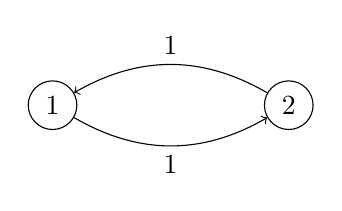
\begin{tikzpicture}
		\tikzstyle{line node} = [draw, fill=white, font=\footnotesize ]
	    \node[shape=circle,draw=black] (1) at (0,0) {1};
	    \node[shape=circle,draw=black] (2) at (3,0) {2};
	    \path [->](1) edge[bend right] node[midway,below] {$1$} (2);
	    \path [->](2) edge[bend right] node[midway,above] {$1$} (1);
	\end{tikzpicture}
\end{equation*}
Starting from $X_0=1$, it will be in state 1 at all even times and in state 2 at odd times — this chain is \emph{periodic}.
As a result, $p(X_t = i)$ alternates between 0 and 1 and does not converge over time.
But even though it has no limiting distribution, it does have a stationary distribution $\vecpi^\star = (\nicefrac{1}{2}, \nicefrac{1}{2})$, as is easily verified.




Here more more common thing that can go ‘wrong’: sinks can lead to multiple stationary distributions. 
Consider two connected copies of our weather model:
\begin{equation*}
	\begin{tikzpicture}
		\tikzstyle{line node} = [draw, fill=white, font=\footnotesize ]
	    \node[shape=circle,draw=black] (1) at (0,0) {1};
	    \node[shape=circle,draw=black] (2) at (2,0) {2};
	    \node[shape=circle,draw=black] (3) at (4,0) {3};
	    \node[shape=circle,draw=black] (4) at (6,0) {4};
	    \node[shape=circle,draw=black] (5) at (8,0) {5};
	
	    \path [->](1) edge[bend right] node[midway,below] {$\nicefrac{1}{2}$} (2);
	    \path [->](2) edge[bend right] node[midway,above] {$1$} (1);
	    \path [->](1) edge[out=135,in=225,looseness=8] node[midway,left] {$\nicefrac{1}{2}$} (1);
	    \path [->](3) edge node[midway,above] {$\nicefrac{1}{4}$} (2);
	    \path [->](3) edge node[midway,above] {$\nicefrac{3}{4}$} (4);
	    \path [->](4) edge[bend right] node[midway,below] {$\nicefrac{1}{2}$} (5);
	    \path [->](5) edge[bend right] node[midway,above] {$\nicefrac{1}{2}$} (4);
	    \path [->](5) edge[out=45,in=315,looseness=8] node[midway,right] {$1$} (5); 
	\end{tikzpicture}
\end{equation*}
If the chain at some point reaches node $2$ it will keep jumping between 1 and 2 afterwards. $\{1,2\}$ thus acts like a ‘sink’ from which there is no escape.
The set $\{4,5\}$ is another such sink.
Both sinks having their ‘own’ stationary distributions and
depending on the initial condition, the chain converges to one of them — or a mixture. 
Concretely, write $\delta_i$ for degenerate and deterministic distribution with all mass on state $i$.
If we start with the initial distribution $\vecpi_0 = \delta_1$, the chain converges to the stationary distribution $(\nicefrac{2}{3}, \nicefrac{1}{3}, 0, 0, 0)$.
But if we start on the other side with $\vecpi_0 = \delta_5$, then it converges to $(0,0,0,\nicefrac{1}{3}, \nicefrac{2}{3})$.
Finally, starting in the middle with $\vecpi_0 = \delta_3$ results in a mixture of both: $(\nicefrac{2}{12}, \nicefrac{1}{12}, 0, \nicefrac{3}{12}, \nicefrac{6}{12})$.
All of these are stationary distributions. 
(And so are all the convex combinations of $(\nicefrac{2}{3}, \nicefrac{1}{3}, 0, 0, 0)$ and $(0,0,0,\nicefrac{1}{3}, \nicefrac{2}{3})$.)




In this case, there is no unique stationary distribution because the graph has several sinks from which one cannot reach the other parts of the graph.
If \emph{every} state is reachable from every other state with positive probability in a finite number of steps, then it is called \emph{irreducible}.
Such a Markov chain has no sinks and every state will almost surely be visited again and again.\footnote{%
	%>>>
		This is generally not true for infinite state spaces, but introduced as an additional condition (\emph{recurrence})
	%<<<
	}
It (almost) never stops visiting the \emph{entire} state space.
	



%——————————————————————————————————————————————————————————
\paragraph{ergodicity}

Markov chains that are both irreducible and aperiodic are said to be \emph{ergodic}.
Together, the two properties are sufficient to ensure convergence of a Markov chain to a unique stationary distribution, just as in our weather model:
\begin{theorem}[1.8.3 in \cite{Norris1997}]
	\label{thm:convergence}
	Let $(x_0, x_1, \dots)$ be an ergodic Markov chain with initial distribution $\vecpi$, transition matrix $\mathbf{T}$ and stationary distribution $\vecpi^\star$. Then
	\begin{equation}
		p(x_n = i) \longrightarrow \pi_j^\star \quad \text{as} \quad n \longrightarrow \infty
	\end{equation}
	for all $i\in S$.
\end{theorem}




As we have seen, an ergodic Markov chain over time traverses the entire state space in an aperiodic fashion.
One might wonder if any regularity underlies the states it visits. 
Is it more likely to visit high-probability states under the stationary distribution, for example?
Indeed, it is.
The relative frequencies of visited states in fact converge to the stationary distribution. 
The important point is that this connects a distribution \emph{over time} — the visited states — with a distribution \emph{over the state space} — the stationary distribution.
\emph{Ergodic theory} studies this relation between time- and space-averages and I want to state one result here.
To do so we define these averages, for any bounded function $f: S \to \mathbb{R}$, as
\begin{equation}
	f_{\text{time}}	:= \frac{1}{n}\sum_{k=0}^{n-1} f(X_k)
		\quad\text{and}\quad
	f_{\text{space}} := \sum_{i\in S} \vecpi^\star_i f(i)
\end{equation}
The result is as follows.
\begin{theorem}[Ergodic Theorem; 1.10.2 in \cite{Norris1997}]
	Let $(x_n)_{n\ge 0}$ be as in theorem \ref{thm:convergence} and let $f: S \to \mathbb{R}$ be any bounded function. Then the time-average of $f$ almost surely converges to the space-average of $f$:
	\begin{equation}
		p\bigl(f_{\text{time}} \longrightarrow f_{\text{space}} \quad \text{as}\quad n \longrightarrow \infty \bigr) = 1.
	\end{equation}
\end{theorem}




I omit the proof, but want to draw a practical conclusion.
As seen, one can find the stationary distribution as an eigenvector of (an estimate of) the transition matrix, but the previous theorem shows a more intuitive option: measuring relative frequencies.
If $V_i(t)$ is the number of visits to state $i$ before time $t$, then $f_i(t) = V_i(t) / t$ is the relative frequency.
For an ergodic Markov chain, this converges to the stationary distribution,
$f_i(t) \to \pi_i$ as $t\to\infty$, with probability 1.
This is (a consequence of) the Ergodic theorem \parencite[][1.10.2]{Norris1997} when $f_i$ is the indicator function.
As the reader might notice, this fact has been used extensively.



%——————————————————————————————————————————————————————————
\showbibliography



\end{document}
	
	% Appendix Lateral Inhibition strategies
	\documentclass{../src/bcthesispart}
\title{Lateral Inhibition Strategies}
\author{Bas Cornelissen}
\begin{document}

%——————————————————————————————————————————————————————————
\appendixtitle{Lateral Inhibition Strategies}{Lateral Inhibition Strategies}{li-strategies}{%
	%
	% Abstract
	% ————————
	In chapter \ref{ch:naming-games} we explored five different lateral inhibition strategies, and concluded that they always converge to an effective, shared language.
	Do these conclusions indeed generalize to the rest of the 6-dimensional, strategy space?
	The convergence proof suggests so, but does not apply to the naming games directly. 
	In this appendix part of the parameter space is therefore explored systematically.
	The results indicate that effective languages eventually emerge for all strategies, although the dynamics before convergence can vary substantially.
}
%——————————————————————————————————————————————————————————


\noindent
Recall that the space of lateral inhibition strategies is defined by five nonnegative parameters
\begin{equation}
	\delta_{\text{inc}}, \quad
	\delta_{\text{inh}}, \quad
	\delta_{\text{dec}}, \quad
	s_{\text{init}}, \quad 
	s_{\text{max}}.	
\end{equation}
I have not been able to find a systematic analysis of the parameter space.
\textcite{Wellens2012} does compare several strategies and suggest that the the value of the parameters determines the strategy. 
For example concluding that “a higher value [of $\delta_{\text{inh}}$] improves alignment”.
I belief this is slightly inaccurate, since the strategies are invariant under scaling.
In other words, it is the \emph{relative} value of the parameters that matters.
There are many more such equivalences.
%Translating $\delta_{\text{init}}, s_{\text{min}}$ and $s_{\text{max}}$ for example does not alter a strategy.
One could for example use any other
$\delta_{\text{inh}} \ge s_{\text{init}}$ without altering the minimal strategy; or fix $s_{\text{max}} := s_{\text{init}}$ and use any $\delta_{\text{inc}}>0$.
Similarly, a different $\delta_{\text{inc}} > 0$ leaves the frequency strategy unchanged, since scores greater than $s_{\text{init}}$ are of the form $s_\text{init} + k\cdot \delta_{\text{inc}}$ and essentially track the frequency $k$ anyway.




%- - - - - - - -
\begin{SCfigure}
	\includegraphics[trim=1.26cm 0 0 \figtopmargin]{LING03-02-combined-results}
	\caption{\subfig{A} The effect of $\delta_{\text{inh}}$ keeping $\delta_{\text{inc}} = 1$ fixed. It interpolates between the minimal strategy and frequency strategy. \subfig{B} the effect of $\delta_{\text{inc}}$ for $\delta_{\text{inh}} = 1$ fixed. For large $\delta_{\text{inc}}$, the inhibition is rendered ineffective.
		\figdetails{\figid{LING03}
		Results shown for $N=200$, $\delta_{\text{dec}} = 0$, $s_{\text{init}} = 1$, $s_{\text{max}} = \infty$; avg.\ of 300 runs. $p_{\text{success}}$ is moreover a rolling average over a centered window of 1000 iterations.
		}
		\label{fig:delta-inh-vs-delta-inc}}
\end{SCfigure}
%- - - - - - -




We map two slices of the strategy space by fixing either the increments or inhibition parameter and varying the other \parencite[following][]{Wellens2012}.
Figure \ref{fig:delta-inh-vs-delta-inc} reports the results.
Fixing $\delta_{\text{inc}} = 1$ while varying $\delta_{\text{inh}}$ (figure \ref{fig:delta-inh-vs-delta-inc}\textsc{a}) reveals that the inhibition parameter $\delta_{\text{inh}}$ interpolates between the minimal strategy ($\delta_{\text{inh}} = 4^2$ or larger; purple) and and the frequency strategy ($\delta_{\text{inh}} = 0$; black).
Both reach eventually reach perfect communicative success, but the stronger the lateral inhibition, the faster so.
The number of unique words $N_{\text{unique}}$ initially grows identically for all $\delta_{\text{inh}}$ as inhibition plays hardly any role at the start of the game.
In the frequency strategy, no words are ever removed and the resulting vocabulary is therefore not \emph{efficient}.
It is hard to tell if the amount of lateral inhibition matters in the long-term. The plot seems to suggest that this is not the case, and even the slightest lateral inhibition will (after a significantly longer time) result in a one-word language.




The effect of the increment $\delta_{\text{inc}}$ is shown in figure \ref{fig:delta-inh-vs-delta-inc}\textsc{b}.
One can see that the minimal strategy corresponds to $\delta_{\text{inc}} = 0$, but larger increments yield different dynamics.
After the peak of $N_{\text{unique}}$, words with score $\delta_{\text{init}} = 1$ are quickly removed, as it takes a single inhibition.
But words that have been heard multiple times have scores of at least $\delta_{\text{init}} + \delta_{\text{inc}}$ and need many more inhibitions to be removed.
There appear to be around $\nicefrac{N}{6}$ such words.
The result is a temporary stabilisation of $N_{\text{unique}}$.
Eventually inhibition takes over and competing words start disappearing. 
The (very) long-term behaviour thus appears to be the same as before: convergence to a single-word language.

%
%The take home message seems to be this: all strategies we have discussed give rise to a shared convention that allows the population to name the object.
%If there is any form of lateral inhibition, the stable language will have only a single word as all competing words will have been removed.
%Indeed, a shared single word language is a stable state: no words need to be invented and there are no words to inhibit.
%The only strategy with different stable states is the frequency strategy.
%There \emph{all} invented words spread the population, but since agents use the most frequent word, they can still communicate effectively.
%The precise dynamics leading to the stable stable state depends on the parameter settings.
%Communicative success can increase faster, slower or even stabilise temporarily, but will eventually be reached nonetheless.


%——————————————————————————————————————————————————————————
\showbibliography


\end{document}

	% Appendix mathematical details BNG
	\input{../10-app-bayesian-ng/appendix-bayesian-ng}

	% Appendix BNG illustrations
	\documentclass{../src/bcthesispart}
\title{Parameter space of the \textsc{dc} language game}
\author{Bas Cornelissen}
\begin{document}

%——————————————————————————————————————————————————————————
\appendixtitle{Parameter space of the \textsc{dc} language game}%
	{Parameter space of the \textsc{dc} language game}%
	{bng-params}{%
	% Abstract
	%---------
	The Bayesian language game has a language strategy parameter $\eta$, a production strategy parameter $\zeta$ and a parameter $\gamma$ for the life expectancy.
	How do those influence the resulting behaviour of the model? 
	This appendix reports an experiment that systematically analysed the behaviour in a larger part of the space.
	}
%——————————————————————————————————————————————————————————

	

The experiment measures three new quantities besides coherence and reflectance
The first concerns the amount of \emph{synonymy} in the language.
If a language assigns all words the same probability, the synonymy is maximal, but if one word takes all probability mass, there is no synonymy. 
Synonymy is the inverse notion of efficiency in the naming games and formally defined as the relative Shannon entropy of the aggregate language,
%-
\begin{align}
	S(t) := 
		\frac{H( \bar{\vect\pi}_t )}%
		{\log_2(N)},
\end{align}
%-
where $H$ is the entropy. $S(t) = 1$ indicates maximal synonymy, $S(t) = 0$ the complete absence of synonymy.
Second, the \emph{discrepancy} between the internal and external language is measured:
%-
\begin{equation}
	D(t) :=
		\textsc{jsd}(\bar{\vect\pi}_t, \vect\psi_t),
\end{equation}
%-
where the aggregate language functioned as a proxy of all internal languages.
Third, we measure the \emph{variability} of the aggregate language as its standard deviation over time,
%-
\begin{align}
	V(t) = \text{std}(\bar{\vect\pi}_0, \dots, \bar{\vect\pi}_t).
\end{align}
%-
If the languages used in the populations were relatively stable throughout the game, the variability should be low.
%%





The experiment simulated 20 runs of the Dirichlet-categorical language game for every combination of the parameters $\eta \in \{1, 2, 5, 50, \infty\}	$, $\zeta \in \{1, 1.5, 2, 5, \infty\}$ and $\gamma \in \{ 1, 10, 50, 10, 100, 1000, \infty \}$.\footnote{%
	%>>>
	To be completely clear: that amounts to 350 million rounds in 3500 independent simulations, using 175 different parameter settings.
	%<<<
	} 
Every run had a duration of 100 000 iterations and all used the same, relatively flat, but nonuniform, prior.
Trial experiments suggested that these parameter values sufficiently illustrate games in different parts of the parameter space.
For example, $\eta>100$ and $\zeta>100$ already yield behaviour comparable to the infinite case and were left out.
The coherence,\footnote{%
	%>>>
	Coherence is not shown, because all simulations appear to have reached coherence.
	This is an artefact of the measure used, which should thus be improved: populations with few observations, as in iterated learning, look perfectly coherent to our measure, because the shared bias fully determines their language.
	%<<<
} reflectance, synonymy, discrepancy, and variability were measured at the end of every game.
Figure \ref{fig:BNG06-parameter-space} shows all the results.
Interpreting the results is tricky, and it helps to keep figure \ref{fig:FIG08-bng-overview} in mind:
The corners of every heat map in figure \ref{fig:BNG06-parameter-space} mark the extreme strategies ($\eta,\zeta\in\{1, \infty\}$), which were also shown in figure \ref{fig:FIG08-bng-overview}.
The life expectancies we considered earlier ($\gamma=1, 10, 100$ and $\infty$) can also be found in figure \ref{fig:FIG08-bng-overview}.
Now, the main conclusion is be that \emph{our earlier findings are largely confirmed by the current experiment.}
For intermediate parameter values, we observe a relatively smooth transition between the extreme cases $\eta,\zeta,\gamma\in\{1,\infty\}$.




%- - - - - - - - 
\begin{SCfigure}
	\includegraphics[trim=1.36cm 0 0 \figtopmargin]{BNG06-parameter-space}
	\caption{%
	The behaviour of the Dirichlet-categorical language game across the parameter space $(\gamma,\eta,\zeta)$.
	Rows corresponds to life expectancies ($\gamma$); columns show the coherence, reflectance, synonymy and variability for every strategy $(\eta, \zeta)$.
	See figure \ref{fig:FIG08-bng-overview} for the typical resulting languages in the extreme cases $\gamma,\eta,\zeta \in \{1, \infty\}$.
	%----------
	\figdetails{\figid{bng06}
	Every cell is an average over 20 simulation runs. $K=20$, $N=10$, $b=1$, $\gamma=\infty$, $\beta=30$. 
	Simulations used a deterministic hazard function.}
	\label{fig:BNG06-parameter-space}}
	%todo (optional) highlight extreme cases in plot
\end{SCfigure}
%- - - - - - - - 


We first discuss the last row, which corresponds to a naming game.
The reflectance (column \textsc{a}) is much higher for samplers, and decreases quickly as soon as agents start to maximise their productions slightly (i.e. $\zeta > 1$). 
The synonymy (column \textsc{b}) suggests why: maximising production strategies result in a one-word language, that is, one with no synonymy.
This explains why the reflectance is low for high $\zeta$: the bias allows much more synonymy.
The reflectance and synonymy also suggest that the language strategy ($\eta$) is far less influential than the production strategy ($\zeta$).
The fact that the change in vertical direction is smaller than the change in horizontal direction, and this seems to generalise to other life-spans as well.
Looking at agents with shorter lifespans, we further see that the reflectance and synonymy increase as $\gamma$ approaches 1 (iterated learning).
As before, the reason is that the internal language of an agents with a short life span is nearly completely determined by the bias.
Accordingly, reflectance is high and since the bias is fairly flat, so is synonymy.
But, note that the discrepancy between the external language and the internal  increases sharply for more maximising strategies.
Finally the last column shows an increase in variability with intermediate lifespans. 
This could indicate continuous language change when agents have an intermediate lifespan of around $\gamma=1000$ interactions, but more research is needed before such conclusions are warranted.
%this cannot be concluded yet with any certainty

%Nevertheless, the reflectance and synonymy is largely comparable to the naming-game case ($\gamma=\infty$).
%This suggests that the language is fairly stable, but changes slowly within the constraints set by the bias.




\end{document}

	
	\documentclass{../src/bcthesispart}
\title{A discrete Weibull model of population turnover}
\author{Bas Cornelissen}
\begin{document}

%——————————————————————————————————————————————————————————

\appendixtitle{A discrete Weibull model of population turnover}%
	{A discrete Weibull model of population turnover}%
	{weibull}{%
	%
	% Abstract
	% ————————
	Population turnover is commonly modelled by replacing one random agent in every round. 
	Such a constant mortality rate is not very realistic, and this appendix proposes an alternative, discrete Weibull model.
	It is reparametrised such that the mean life expectancy is the only parameter.
}

%——————————————————————————————————————————————————————————




\noindent
How can we realistically model the mortality-rate in a population?
This is a central question in \emph{survival analysis} \parencite[e.g.][]{Rodriguez2007}.
In the context of a model of language evolution, if one agent dies in every iteration, the probability that any given agent dies at time $t$ is thus $\gamma$ — \emph{given that it was still alive at time $t-1$}.
If $T$ is the random variable that measures the time of death of an agent, this means $p(T = t \mid T \ge t) = \gamma$.
This conditional probability is known as the \emph{hazard rate} $h(t)$, as it measures the rate of death (hazard) occurring at $t$.\footnote{%
	%>>>
	It is usually defined for continuous $T$ with density $f$ as $h(t) = \frac{f(t)}{1-F(t)}$, in which case it is not a conditional probability but the \emph{rate} of instantaneous hazard.
	%<<< 
	}
In our example the hazard rate was constant.
But, as explained in chapter \ref{ch:bayesian-naming-games}, models with constant hazard rates are poor models of life-expectancy in human populations and demographers usually adopt either the \emph{Weibull} or \emph{Gompertz} distribution \parencite{Juckett1993}.
We here consider the simpler Weibull distribution, mainly because several discrete analogous have been proposed \parencite{Nakagawa1975,Stein1984,Almalki2014}.




%——————————————————————————————————————————————————————————
\paragraph{Discrete Weibull distribution} 

The Weibull distribution \parencite{Weibull1951} is a continuous distribution parametrized by a scale parameter $\kappa>0$ and a shape parameter $\lambda>0$. 
If $\kappa>1$ the distribution is unimodal, meaning that most agents die around the same age, which is in turn determined by $\lambda$ (see figure \ref{fig:weibull-params}).
For completeness, the density of a Weibull-distributed random variable $T$ is
\begin{align}
	p(t \mid \lambda, \kappa) = \nicefrac{\kappa}{\lambda} \cdot \bigr(\nicefrac{t}{\lambda}\bigl)^{\kappa-1} \cdot \;\text{exp}\Bigl(-\bigr(\nicefrac{t}{\lambda}\bigl)^{\kappa}\Bigr).
\end{align}
Since language games are discrete time models, we use a discrete approximation known as the \emph{Discrete Weibull} distribution\footnote{I reparametrized the distribution by taking $\beta := \kappa$ and $q := \text{exp} ( - \lambda^{-\kappa})$, which is both computationally and conceptually more convenient.}\parencite{Nakagawa1975}, which preserves the so called \emph{survival} function of the continuous distribution.
The \emph{survivor} function $S(t) = p(T \ge t)$ measures the probability of surviving to at least time $t$.
The Weibull distribution, this function takes the form
\begin{equation}
	S(t) = \text{exp}\Bigl(	-\bigl(\nicefrac{t}{\lambda}\bigr)^k\Bigr),
\end{equation}
and the Discrete Weibull is defined as the discrete distribution with the same survival function.
This can be done, since the probability mass function is fully determined by the survival function:
\begin{equation}
p(T = t) = S(t) - S(t+1) = \text{exp}\Bigl(	- \bigl(\nicefrac{t}{\lambda}\bigr)^\kappa \Bigr) - \text{exp}\Bigl(- \bigl(\nicefrac{t+1}{\lambda}\bigr)^\kappa\Bigr).
\end{equation}
It should be stressed that the resulting distribution \emph{approximates} the Weibull distribution, which for our purposes is sufficient.




The hazard rate of the Discrete Weibull distribution can be computed as
\begin{align}
	h(t) 
		= p(T= t \mid T\ge t)
		= \frac{S(t) - S(t+1)}{S(t)}
		= 1 - \text{exp}\Bigl( \bigl(\nicefrac{t}{\lambda}\bigr)^{\kappa} -  \bigl(\nicefrac{t+1}{\lambda}\bigr)^{\kappa}\Bigr).
\end{align}
Recall that the hazard rate is the probability that an agent dies at time $t$, given that it hasn’t died yet. 
Therefore, if we want to model a population where the probability of dying at time $T$ approximately follows a Weibull distribution, we should in every round flip a coin with weight $h(t)$ to decide whether the agent dies. 




%- - - - - - - -
\begin{SCfigure}
	\includegraphics[trim=1.2cm 0 0 \figtopmargin]{FIG04-Weibull-params}
	\caption{
	The Weibull distribution can model the probability that an agent dies at time $t$.
	\subfig{A} Varying the parameters of a Weibull distribution illustrates that $\lambda$ is a scale parameter and $\kappa$ a shape paramater.
	\subfig{B} If $\kappa>1$ the Weibull is a unimodal distribution, whose variance decreases with higher $\kappa$ (thinner lines), but for $\kappa<1$ the distribution has no mode.
	When $\kappa=1$ the Weibull reduces to a exponential distribution.
		\figdetails{\figid{fig04}}
		\label{fig:weibull-params}}
\end{SCfigure}
%- - - - - - - -

%- - - - - - - -
\begin{SCfigure}
	\includegraphics[trim=1.33cm 0 0 \figtopmargin]{FIG04-continuous-discrete-Weibull}
	\caption{The single-parameter version of the continuous and discrete Weibull distribution. 
		\subfig{A} The distributions closely line up and $\gamma$ is easily interpretable. 
		\subfig{B} The hazard rate increases with time, thus capturing ageing effects. 
		Note that a continuous hazard rate $h(t)$ is not a distribution and exceeds 1.
		\figdetails{\figid{fig04}}
		\label{fig:cont-discr-weibull}}
\end{SCfigure}
%- - - - - - - -




%——————————————————————————————————————————————————————————
\paragraph{Modelling population turnover}

The Discrete Weibull gives us a more realistic model of population turnover, but its behaviour is regulated by two parameters: $\lambda$ and $\kappa$.
Ideally a \emph{single} parameter would interpolate between immediate death (iterated learning) and immortality (naming game).
This can be done by defining $\lambda$ and $\kappa$ in terms of a $\gamma \ge 1$:
\begin{align}
	\kappa(\gamma) := \log(\gamma) + \kappa_0
	\qquad\text{and}\qquad
	\lambda(\gamma) := \frac{\gamma}{\Gamma\bigl(1 + \nicefrac{1}{\kappa(\gamma)}\bigl)}, \qquad \gamma\ge1
\end{align}
where $\Gamma$ is the gamma function. 
Figure \ref{fig:cont-discr-weibull} illustrates the effect of $\gamma$.
Three reasons underly this reparametrization. 
First, the term $\Gamma\bigl( 1 + \nicefrac{1}{\kappa(\gamma)}\bigl)$ makes $\gamma$ interpretable: $\gamma$ is the mean of the continuous distribution $\text{Weibull}\bigl(\lambda(\gamma), \kappa(\gamma)\bigl)$.
Second, scaling $\kappa(\gamma)$ logarithmically with $\gamma$ results in a realistic mortality distribution for all $\gamma\ge 1$.
Third, the constant $\kappa_0$ guarantees that for $\gamma=1$ the hazard rate is approximately 1, corresponding to instant death in iterated learning. I opt for\footnote{This results in the hazard rate $h(1 \mid \lambda=1) > 1 - 10^{-8}$, which seems sufficiently close to 1.} $\kappa_0 = 5$.




In sum, we have defined a discrete Weibull model, approximating the continuous Weibull, but parametrised by a single parameter $\gamma$, the average life expectancy. 
When used in combination with a random walk through a population of fixed size, $\gamma$ thus interpolates between iterated learning ($\gamma=1$) and a naming game ($\gamma=\infty$).




%——————————————————————————————————————————————————————————
\showbibliography

\end{document}

	
	% Appendix Packing Strategy
	\documentclass{../src/bcthesispart}
\title{Reformulating the packing strategy}
\author{Bas Cornelissen}
\begin{document}

%——————————————————————————————————————————————————————————

\appendixtitle{Reformulating the packing strategy}%
	{Reformulating the packing strategy}%
	{packing-strategy}{%
	%
	% Abstract
	% ————————
	The technical formulation of the packing strategy in \parencite{Hurford1975} seems to have caused some confusion in the literature.
	This appendix reformulates the principle independent of the original generative framework, without compromising preciseness.
	This will bring some limitations of the packing strategy to the fore.
}

%——————————————————————————————————————————————————————————


%——————————————————————————————————————————————————————————
\paragraph{The packing strategy as a constraint on trees}

The packing strategy was introduced within the conceptual framework of generative grammar, as a ‘significant generalisations’ about number expressions and how they relate to numbers.
\textcite{Hurford1975} analysed several numeral systems (English, French, Danish, Mixtec and Yoruba) using a phrase structure grammar which can be simplified to:\footnote{%
	%>>>
	The original phrase structure rules constructed bases using exponentiation. 
	This is controversial (see chapter \ref{ch:numerals}) so I have use the most recent, simplified grammar from \textcite{Hurford2007}.
	Note that the rewrite rule of \PROD{} is different in \textcite{Hurford1987}, where \SUM{} is not optional.
	I have also changed notation and use \SUM{} for \textsc{num}; \PROD{} for \textsc{phrase}; and \ATOM{} for \textsc{digit}.
	%<<<
	}
%-
\begin{align}
	\label{eq:app-ps:hurford-grammar}
	%-----
	\begin{split}
		\text{\SUM} 
			&\longrightarrow \begin{Bmatrix*}[l]
				\text{\ATOM}\\
				\text{\PROD{} (\SUM)}
			\end{Bmatrix*}
		\\
		\text{\PROD} 
			&\longrightarrow \;\text{(\SUM) \BASE}
	\end{split}
\end{align}
%-
where \ATOM{} and \BASE{} rewrite to one of the atoms and bases of the system respectively.
It is easiest to think of this grammar as an \emph{attribute grammar} \parencite{Knuth1968} where every leaf (\ATOM{} or \BASE{}) has a fixed numeric value or \emph{attribute}. 
Every nonterminal node corresponds to an operation that computes the value of the node from the values of its constituents.
\SUM{}s of course correspond to sums and \PROD{}s to products.
Here is the structure for French \lng{quatre-vingt-dix-sept}, where I decorated nodes with their attributes in grey:
%-
\begin{align}
	\label{eq:app-ps:tree-quatre-vingt-dix-sept}
	%-----
	\begin{tikzpicture}[frontier/.style={distance from root=10em}]
		\Tree 
		[.\SUM{}\attr{97} 
			[.\PROD{}\attr{80} 
				[.\SUM\attr{4} [.\ATOM{}\attr{4} quatre ] ]
				[.\BASE{}\attr{20} vingt ] ]
			[.\SUM{}\attr{17} 
				[.\PROD{}\attr{10} 
					[.\BASE{}\attr{10} dix ] ]
				[.\SUM{}\attr{7} 
					[.\ATOM{}\attr{7} sept ] ] ] ]
	\end{tikzpicture}
\end{align}
%-
%%




This is just one of the many structures with value 97 generated by the rules \eqref{eq:app-ps:hurford-grammar}. 
The packing strategy was introduced as a way to separate the wellformed from the illformed structures.
It was therefore formulated as constraint on the structure of the trees, namely that:\footnote{%
	%>>>
	The formulation is from \textcite{Hurford1987,Hurford2007}. 
	The original also applied to bases constructed by exponentiation and is thus more complicated, as \BASE{} nodes were nonterminals.
	Let $A$ be a structure of category $X$ (i.e.\ a \PROD{} 	or a \BASE{}) with value $x$ and two constituents: a \SUM{} and some node of another category $Z$ (\PROD{} or \BASE{}). 
	Then $A$ is only wellformed if $Z$ has the largest possible value $z \le x$. 
	That is, if there is no alternative $Z'$ that also expands $X$ with $\text{val}(Z) < \text{val}(Z')$.
	%<<<
	}
%-
\begin{align}
	\label{eq:app-ps:packing-strategy}
	%-----
	\text{the sister constituent of a \SUM{} must have the highest possible value.}
\end{align}
%-
That is, the highest possible value while keeping the value of the parent constant.
The sister constituent of a \SUM{} can be a \PROD{} or a \BASE{}. 
Both can be found in \eqref{eq:app-ps:tree-quatre-vingt-dix-sept}: at depth 3 we for example find a \BASE{} with value 20 and a \PROD{} with value 10.
The reader might also have noticed that the node \SUM{}\attr{17} \emph{violates} the packing strategy. 
In a structure of the form
%-
\begin{align}
	\label{eq:app-ps:counterexample-98}
	%-----
	\begin{tikzpicture}
		\Tree 
		[.\SUM{}\attr{97} 
			\PROD{}\attr{90} 
			\SUM{}\attr{7} ]
		\end{tikzpicture}
\end{align}
%-
the node \PROD{}\attr{90} is the sister constituent of a \SUM{} and has a value higher than 80.
We will discuss this problem later in more detail.
%%




The packing strategy also accounts for the order of bases in large numerals, e.g.\ that that \lng{two hundred thousand} is wellformed, but \lng{two thousand hundred} is not:
%-
\begin{align}
	\label{eq:counterexample-98}
	%-----
	\begin{tikzpicture}[frontier/.style={distance from root=15em}]
		\Tree 
		[.\SUM{}\attr{200\;000} 
			[.\PROD{}\attr{200\;000}
				[.\SUM{}\attr{200} 
				 	[.\PROD{}\attr{200} 
				 		[.\SUM{}\attr{2} 
				 			[.\ATOM{}\attr{2} two ] ]
				 		[.\BASE{}\attr{100} hundred ] ] ]	
				[.\BASE{}\attr{1000} thousand ] ] ]
	\end{tikzpicture}
	%
	\hspace{3cm}
	%
	\begin{tikzpicture}[frontier/.style={distance from root=15em}]
		\Tree 
		[.\SUM{}\attr{200\;000} 
			[.\PROD{}\attr{200\;000}
				[.\SUM{}\attr{2000} 
				 	[.\PROD{}\attr{2000} 
				 		[.\SUM{}\attr{2} 
				 			[.\ATOM{}\attr{2} two ] ]
				 		[.\BASE{}\attr{1000} thousand ] ] ]	
				[.\BASE{}\attr{100} hundred ] ] ]
	\end{tikzpicture}
\end{align}
%-
In the tree on the right, the sister node of \SUM{}\attr{2000} is the node \BASE{}\attr{100}, and this violates the packing strategy, as it is also possible to form a tree where the corresponding sister has the higher value 1000. 
This is the tree shown on the left.
%%




%——————————————————————————————————————————————————————————
\paragraph{The packing strategy without trees}

Perhaps the tree representations overly complicated.\footnote{%
	%>>>
	I doubt whether Hurford would disagree; over the years he used ever looser variants of the grammar, and often opts for arithmetic formulae in the discussion \parencite{Hurford1999,Hurford2007}.
	
	%<<<
	}
First they generate obvious redundancies in fragments like
%-
\begin{align}
	\label{eq:chains}
	%-----
	\Tree [.\PROD{}\attr{10} [.\BASE{}\attr{10} dix ] ]
	\qquad\qquad\text{and}\qquad\qquad
	\Tree [.\SUM\attr{4} [.\ATOM{}\attr{4} quatre ] ]
\end{align}
%-	
But more importantly, the same structures can be expressed using simple arithmetic formulae like $(4 \times 20) + (10 + 7)$ and $(2 \times 100) \times 1000$, as we have been doing throughout. More precisely, every tree corresponds to a formula built up from the values of the leaves using the binary operations addition and multiplication.
Such formulae are not only simpler, they also have more expressive power. 
The phrase structure rule can for example only produce multiplicative constructions with a base. 
But as we have seen, languages sometimes contain multiplicative constructions with factors that are \emph{not} considered bases properly: isolated or mixed bases.
Similarly, additive constructions with two atoms are illformed by the packings strategy; a base has to figure in one of the constituents.
The Welsh expression for 15 is an additive base, but not a base. 
This means that \emph{correct} expressions of the form $15+2$ cannot be generated.\footnote{%
	%>>>
	\textcite{Hurford1975} does list 15 as a base, and thus circumvents this at the cost of using an arguably wrong notion of base.
	%<<<
	}
It is furthermore easy to extend the formulae with other (binary) operations like subtraction and division, whereas the phrase structure rules can only account for these using complicated extensions of the semantic interpretation which I will not reproduce here.
Finally, the order of constituents, of the base and atom in particular, cannot be described in the formalism, which is problematic \parencite{Calude2016}. 
In short, the formulae are simpler, more expressive and stay closer to the semantic structure of number expressions.





So how can we express the packing strategy in terms of such formulae?
Well, note that \SUM{}s only occur as sister constituents (bold) in fragments of the form
%-
\begin{align*}
	%(A)
	\text{(a)}
	\Tree [.\SUM{} 
			[.\PROD{} \SUM{} \BASE{} ] 
			\textbf{\SUM{}} ]
	%(B)
	\qquad\quad\text{(b)}
	\Tree [.\SUM{} 
			[.\PROD{} \BASE{} ] 
			\textbf{\SUM{}} ]
	%(C)
	\qquad\quad\text{(c)}
	\Tree [.\PROD{} \textbf{\SUM{}} \BASE{} ]
\end{align*}
%-
which, when collapsing chains, correspond to formulae of the form 
\begin{align*}
	\text{(a)}\;\; (y \times b) + x,\qquad
	\text{(b)}\;\; b + x, \qquad
	\text{(c)}\;\; x \times b.
\end{align*}
Here $x$ is the sum of interest, $y$ some other expresion and $b$ a base. 
Sister constituents of \SUM{}s are thus multiples of bases (considering $b = 1\times b$ a multiple) and the packing strategy states that these should have the highest possible value.
We can thus reformulate the packing strategy as:
%-
\begin{align}
	\label{eq:new-packing-strategy}
	%-----
	\text{Complex numerals use the largest multiple of the largest base possible.}
\end{align}
%-
This directly suggests more general principles, such as:
%-
\begin{align}
	\label{eq:generalized-packing-strategy}
	%-----
	\text{The difference between $a$ and $b$ in $a+b$ and $a\times b$ should be maximised.}
\end{align}
%-
This would also apply to multiplicative constructions like $5 \times 6$, which do not contain a base (in English).
The principle would then correctly favour $3 \times 10$.
Principle (\ref{eq:generalized-packing-strategy}) could be taken as a good interpretation of the informal statement that “languages prefer to form numeral expressions by combining constituents whose arithmetical values are maximally apart, within the constraints defined by the syntax of the system” \parencite[243]{Hurford1987}.
But this is \emph{not} a literal reformulation of the packing strategy: it is slightly more general.
%%




%——————————————————————————————————————————————————————————
\paragraph{Limits of the packing strategy}

One of the arguments for the importance of packing strategy was that it explained the peculiarities of French numerals \textcite{Hurford1975}.
As a final note, I would like to point out that Hurford’s explanation is somewhat problematic.
Recall that structure \eqref{eq:app-ps:counterexample-98} showed that French numerals do not satisfy the packing strategy. 
So how does Hurford use the packing strategy to explain why \lng{soixante dix} ($60 + 10$) is wellformed, and $50+20$ or $40+30$ are not? 
Consider the following expressions for 70:
%-
\begin{align*}
	\begin{tabular}{lll}
		(a) $7 \times 10$				
			& \textbf{(b) $6 \times 10 + 10$}
			& (c) $5 \times 10 + 20$\\
		(d) $3 \times 20 + 10$
			& (e) $2 \times 20 + 3 \times 10$
			&
	\end{tabular}
\end{align*}
%-
The correct expression is (b), although some dialects use \lng{septante} for (a).
We can directly eliminate (c) since the packing strategy favours $(6 \times 10)+10$ over $(5\times 10)+20$.
But (b) is illformed, since  $6 \times 10$ is illformed in the light of $3 \times 20$ (it is assumed that 20 is a base).
To correct for this, two additional constraints are introduced \parencite[101]{Hurford1975}.
The first states (in a complicated way) that $70 \times 10, 80 \times 10$ and $90\times 10$ are illformed. This eliminates (a). 
The second states (in an even more complicated way) that all multiples or 20, except $4 \times 20$, are illformed. 
This eliminates (d) and (e), but also makes (b) \emph{well}formed, as desired.




The Packing Strategy, in short, does not appear to \emph{explain} much about the French numerals.
On the contrary, it would predict a quite different, vigesimal system, which can only be remedied by introducing ad-hoc constraints.
This is perhaps not surprising. 
The packing strategy predicts a completely regular numeral system, and it is hard to see how such a strategy in itself could account for irregularities like those encountered with French numerals.
These conclusions do mean that the packing strategy might not be the important generalisation Hurford suggests it to be.
The corresponding generalisations in \textcite{Greenberg1978} (roughly, 37 and 38) might even be of more empirical relevance.
The latter captures that numeral systems are very predictable, or that “there is no ‘surprise’ in numeral larger than [a certain] base”. 
If the French expression for 70 is irregular, so is the expression for 70 in $170 = 100+70$.
Finally, to the best of my knowledge the packing strategy has never been \emph{systematically} evaluated against a large collection of numeral systems either.
This might be something to address in future work, which might benefit from the simplified formulation of the generalised packing strategy derived in this appendix.


\end{document}

	
	% Appendix counting games
	\documentclass{../src/bcthesispart}
\title{Base games}
\author{Bas Cornelissen}
\begin{document}

%——————————————————————————————————————————————————————————

\appendixtitle{Base games}%
	{Base games}%
	{counting-games}{%
	%
	% Abstract
	% ————————
	This appendix mathematically derives the implicit biases in the additive naming game and presents some further analyses of the parameters of the game.
}

%——————————————————————————————————————————————————————————



%——————————————————————————————————————————————————————————
\subsection{Implicit biases in the additive naming game}

The additive base game strongly favours the use of the highest base.
To quantify that bias, we ask what the probability is that an agent, without any past experience, will use a certain base in the next round.
‘Without past experience’ is important, since we are interested in the \emph{bias}, similar to the Bayesian naming game.
The problem, I think, becomes much more intuitive if you keep the following diagram in mind:





%- - - - - - -
\begin{figure}[h!]
	\centering
	%\documentclass{../src/bcthesispart}
%\begin{document}

\begin{tikzpicture}[yscale=.5,xscale=1]\sffamily\footnotesize

	% Axis with numbers
	\def\axisy{-1.5}
	\foreach \x in {0,...,9} {
		\pgfmathsetmacro{\n}{int(11 + \x)}
		\node at (\x, \axisy-.7) {$\n$};
		
		\draw[dotted] (\x, 4) -- (\x, \axisy);
	}	
	\draw[line width=1] (0,\axisy) -- (9,\axisy);
	\foreach \x in {0,...,9}{
		\draw (\x, \axisy-.15) -- (\x, \axisy+.15);
	}
	\node at (-1,\axisy-.7) {$\mathcal{N}$};

	% x labels for E^{-1}(X)
	\foreach \x in {0,...,4} {
		\pgfmathsetmacro{\n}{int(\x+1)}
		\node[text=main] at (2*\x+.5, 5) {$P_\n$}; 
		\def\d{.35}
		\draw[main] (2*\x-\d,5.7) rectangle (2*\x+1+\d, \x-.7);
	}
	
	% y axis: E(x)
	\foreach \y in {4,...,0} {
		\pgfmathsetmacro{\base}{int(\y+6)}
		\pgfmathsetmacro{\k}{int(\y+1)}
		\node at (-1.4,\y) {$E(b_\k = \base)$};
		
		\pgfmathsetmacro{\xmax}{2*\y+1}
		\draw (0,\y) -- (\xmax, \y);		
		\node[fill, circle, inner sep=0] at (\xmax, \y) {};
		\foreach \x in {0,...,\xmax}{
			\node[fill, circle, inner sep=1.5] at (\x, \y) {};
		}
	}
		
\end{tikzpicture}

%\end{document}

\end{figure}
%- - - - - - -




The diagram illustrates the decimal case $B = 10$, so $K=5$. 
Recall that $E(b)$ is the set of all numbers $n$ in the domain that are expressible with base $b$; 
these sets are shown as horizontal lines with dots at every number $n$.
We first compute the probability $p(n \in E(b_j))$ that we pick a number expressible by the $j$’th base, and then the probability that base $b_j$ is selected \emph{given} that the number is expressible.
From the diagram one directly sees that
%-
\begin{align}
	p\bigl( \; n \in E(b_j) \; \bigr) 
		= \frac{|E(b_j)|}{B} 
		= \frac{j}{K},
\end{align}
%-
which is the relative length of the black line corresponding to $E(b_j)$.
Next, $p(b_j \mid n \in E(x_j))$ has to take into account that other bases might also express $n$. 
Given that $n \in E(b_j)$ there are $j$ \emph{equally likely} ‘parts’ $P_1, \dots, P_j$ that $n$ could have been in. 
The parts correspond the orange boxes.
Now it is easily seen that the numbers $n$ in box $P_j$ can be expressed by $K - j+ 1$ different bases.
In the diagram, the numbers 13 and 14 are in part $P_2$ and can be expressed by $5-2+1 = 4$ different bases.
But that means that
%-
\begin{align}
	p\bigl( \; b_j \mid n \in E(b_j) \; \bigr)
		&= \sum_{i=1}^j 
			p(n \in P_i) 
			\cdot p(b_j \mid n \in P_i)
		\\
		&= \frac{1}{j} 
			\cdot \sum_{i=1}^j \frac{1}{K - i + 1}
		\\
		&= \frac{1}{j} \cdot \Bigl( 
				\sum_{i=1}^K \frac{1}{i} 
				- \sum_{i=1}^{K-j} \frac{1}{i} 
			\Bigr)
		\\
		&= \frac{1}{j} \bigl( H_K - H_{K-j} \bigr),
\end{align}
%-
where $H_n = \sum_{i=1}^n \nicefrac{1}{i}$ is known as the \emph{$n$’th harmonic number} and we assume $H_0 := 0$.
Putting everything together,
%-
\begin{align}
	p(b_j) 
		&= p\bigl( \; n \in E(b_j) \; \bigr)
			\cdot p\bigl( \; b_j \mid n \in E(b_j) \; \bigr)
		\\
		&= \frac{1}{K} \bigl(\; H_K - H_{K-j} \;\bigr).
		%-----
		\label{eq:app-counting-games:bias}
\end{align}
%-
This implies a very strong bias towards using the highest base, which is further discussed in chapter \ref{ch:counting-games}.




As a final check, does \eqref{eq:app-counting-games:bias} really defines a distribution — is it normalised?
The distribution in \eqref{eq:app-counting-games:bias} is normalised if and only if
%-
\begin{align}
	\sum_{j=1}^K \frac{1}{K}(H_K - H_{K-j}) = 1
\end{align}
%-
Multiplying both sides by $K$ and reordering, we see that this is equivalent to
%-
\begin{align}
	\label{eq:app-counting-games:equivalent-formulation}
	%-----
	\sum_{j=1}^{K-1} H_{K-j} = K \cdot (H_K - 1),
\end{align}
%-
where we used the convention $H_{K-K}=H_0 := 0$ to sum only up to $K-1$.
Equation \ref{eq:app-counting-games:equivalent-formulation} is in fact true: it is one of the basic recurrence relations on the  harmonic numbers.
We can therefore conclude that the distribution in \eqref{eq:app-counting-games:bias} is really a distribution.

As a final note, I have note been able to find any reference of this distribution, but I haven’t searched extensively either.
But if the reader happens to recognise this distribution — I would be very interested to learn more about it.



\subsection{Properties of the additive base game}


%——————————————————————————————————————————————————————————
\paragraph{Effect of $\xi$}
Recall that the parameter $\xi$ determined which bases were favoured; base $b$ was \emph{favoured} if 
%-
\begin{align}
	s(b) > 0 
	\qquad \text{and} \qquad 
	s(b) \ge \xi \cdot \max_{b’} s(b’),
\end{align}
%-
for $1 \ge \xi > 0$.
The additive base game was simulated with $\xi \in \{1, \nicefrac{1}{2}, \nicefrac{1}{3}\}$ and the results are reported in figure \ref{fig:app-counting-games:effects-xi}.
The main effect seems to be that lower values of $\xi$ slow down convergence.
This is not surprising: when $\xi=\nicefrac{1}{3}$, an agent only favours a single base if its frequency is 3 times as high as that of any other base.
This is a much weaker preference for frequent bases than with $\xi=1$, in which case agents always use the most frequent base. 




%- - - - - - - -
\begin{SCfigure}
	%% RESULTS HUR02
	\includegraphics[trim=\figleftmarginA{} 0 0 \figtopmargin]{HUR02-results}	
	\caption{Effects of $\xi$, the parameter regulating the production strategy in the additive base game. Clearly, smaller values lead to slower convergence time.
		\figdetails{
			\figid{HUR02}		
			Results shown for $N=200$, $B=10$; avg.\ of 300 runs; 1 std.\ shaded.}
		\label{fig:app-counting-games:effects-xi}}
\end{SCfigure}
%- - - - - - - -


%- - - - - - - -
\begin{SCfigure}
	% Results HUR01b
	\includegraphics[trim=\figleftmarginA{} 0 0 \figtopmargin]{HUR01-results}	
	\caption{The effect of $K$, the number of bases, in the additive base game. 
		\figdetails{
			\figid{HUR01}
			Results shown for $N=200$, $\xi=1$; avg.\ of 300 runs; 1 std.\ shaded.}
		\label{fig:app-counting-games:effect-B}}
\end{SCfigure}
%- - - - - - - -




%——————————————————————————————————————————————————————————
\paragraph{effects of the number of simple numerals}

How does the number of simple numerals influence the game?
Figure \ref{fig:app-counting-games:effect-B} summarises some experiments of the additive base game with $B \in \{1,10,20,30\}$.
Although these simple experiments do not yield strong conclusions, the convergence time is not strongly influenced by $B$.
That is, certainly not in a power law fashion, like population size.
Rather, the convergence time does not seem to depend on $K$.
One reason for this is that convergence time in the Dirichlet-categorical naming game was also not found to be strongly influenced by $K$.



%——————————————————————————————————————————————————————————
\showbibliography

\end{document}

\end{subappendices}

% Bibliography

{% Appendices page
	\sffamily%
	\addchap{Bibliography}
	\thispagestyle{empty}
}

%\setlength{\bibsep}{0pt plus 0.3ex}
\setlength\bibitemsep{0pt}
%\setlength\bibhang{.\parindent} % default value: \parindent
\renewcommand*{\bibfont}{\footnotesize}

%\begin{multicols}{2}
{\footnotesize\raggedright \printbibliography[heading=none]}
%\end{multicols}

\mbox{}
\thispagestyle{empty}
\newpage

\mbox{}
\thispagestyle{empty}
\newpage


\end{document}
